% Chapter, Section, Figure, Table, Theorem, Corollary, Lemma, Definition, {\bf       
\chapter{Finite-State Transducers}\label{ch-7}

We have seen that finite-state acceptors are by no means robust enough to accept
standard computer languages like Pascal. Furthermore, even if a DFA could
reliably recognize valid Pascal programs, a machine that only indicates ``Yes,
this is a valid program'' or ``No, this is not a valid program'' is certainly
not all we expect from a compiler. To emulate a compiler, it is necessary to
have a mechanism that will produce some \emph{output} other than a simple yes or
no: in this case, we would expect the corresponding machine language code (if
the program compiled successfully) or some hint as to the location and nature of
the syntax errors (if the program was invalid).

A machine that accepts input strings and \emph{translates} them into output
strings is called a \emph{sequential machine}\index{sequential machine|see{transducer}} or
\emph{\Index{transducer}}. Our conceptual picture of such a device is only
slightly different from the model of a DFA shown in Figure \ref{fig-7.1}a. We still have
a finite-state control and an input tape with a read head, but the accept/reject
indicator is replaced by an output tape and writing device, as shown in Figure
\ref{fig-7.1}b.

These machines do not have the power to model useful compilers, but they can
be employed in many other areas. Applications of sequential machine concepts
are by no means limited to the computer world or even to the normal connotations
associated with ``read'' and ``write.'' A vending machine is essentially a
transducer that interprets inserted coins and button presses as valid inputs and
returns candy bars and change as output. Elevators, traffic lights, and many
other common devices that monitor and react to limited stimuli can be modeled by
finite-state transducers.

The vending machine analogy illustrates that the types of input to a device
(coins) may be very different from the types of output (candy bars). In terms
of our conceptual model, the read head may be capable of recognizing symbols
that are different from those that the output head can print. Thus we will have
an \emph{output alphabet}\index{C@$\Gamma$|see {output alphabet}} $\Gamma$ that is not necessarily the same as
our \emph{input alphabet} $\Sigma$.

% Figure 7.1
\begin{figure}
\centerline{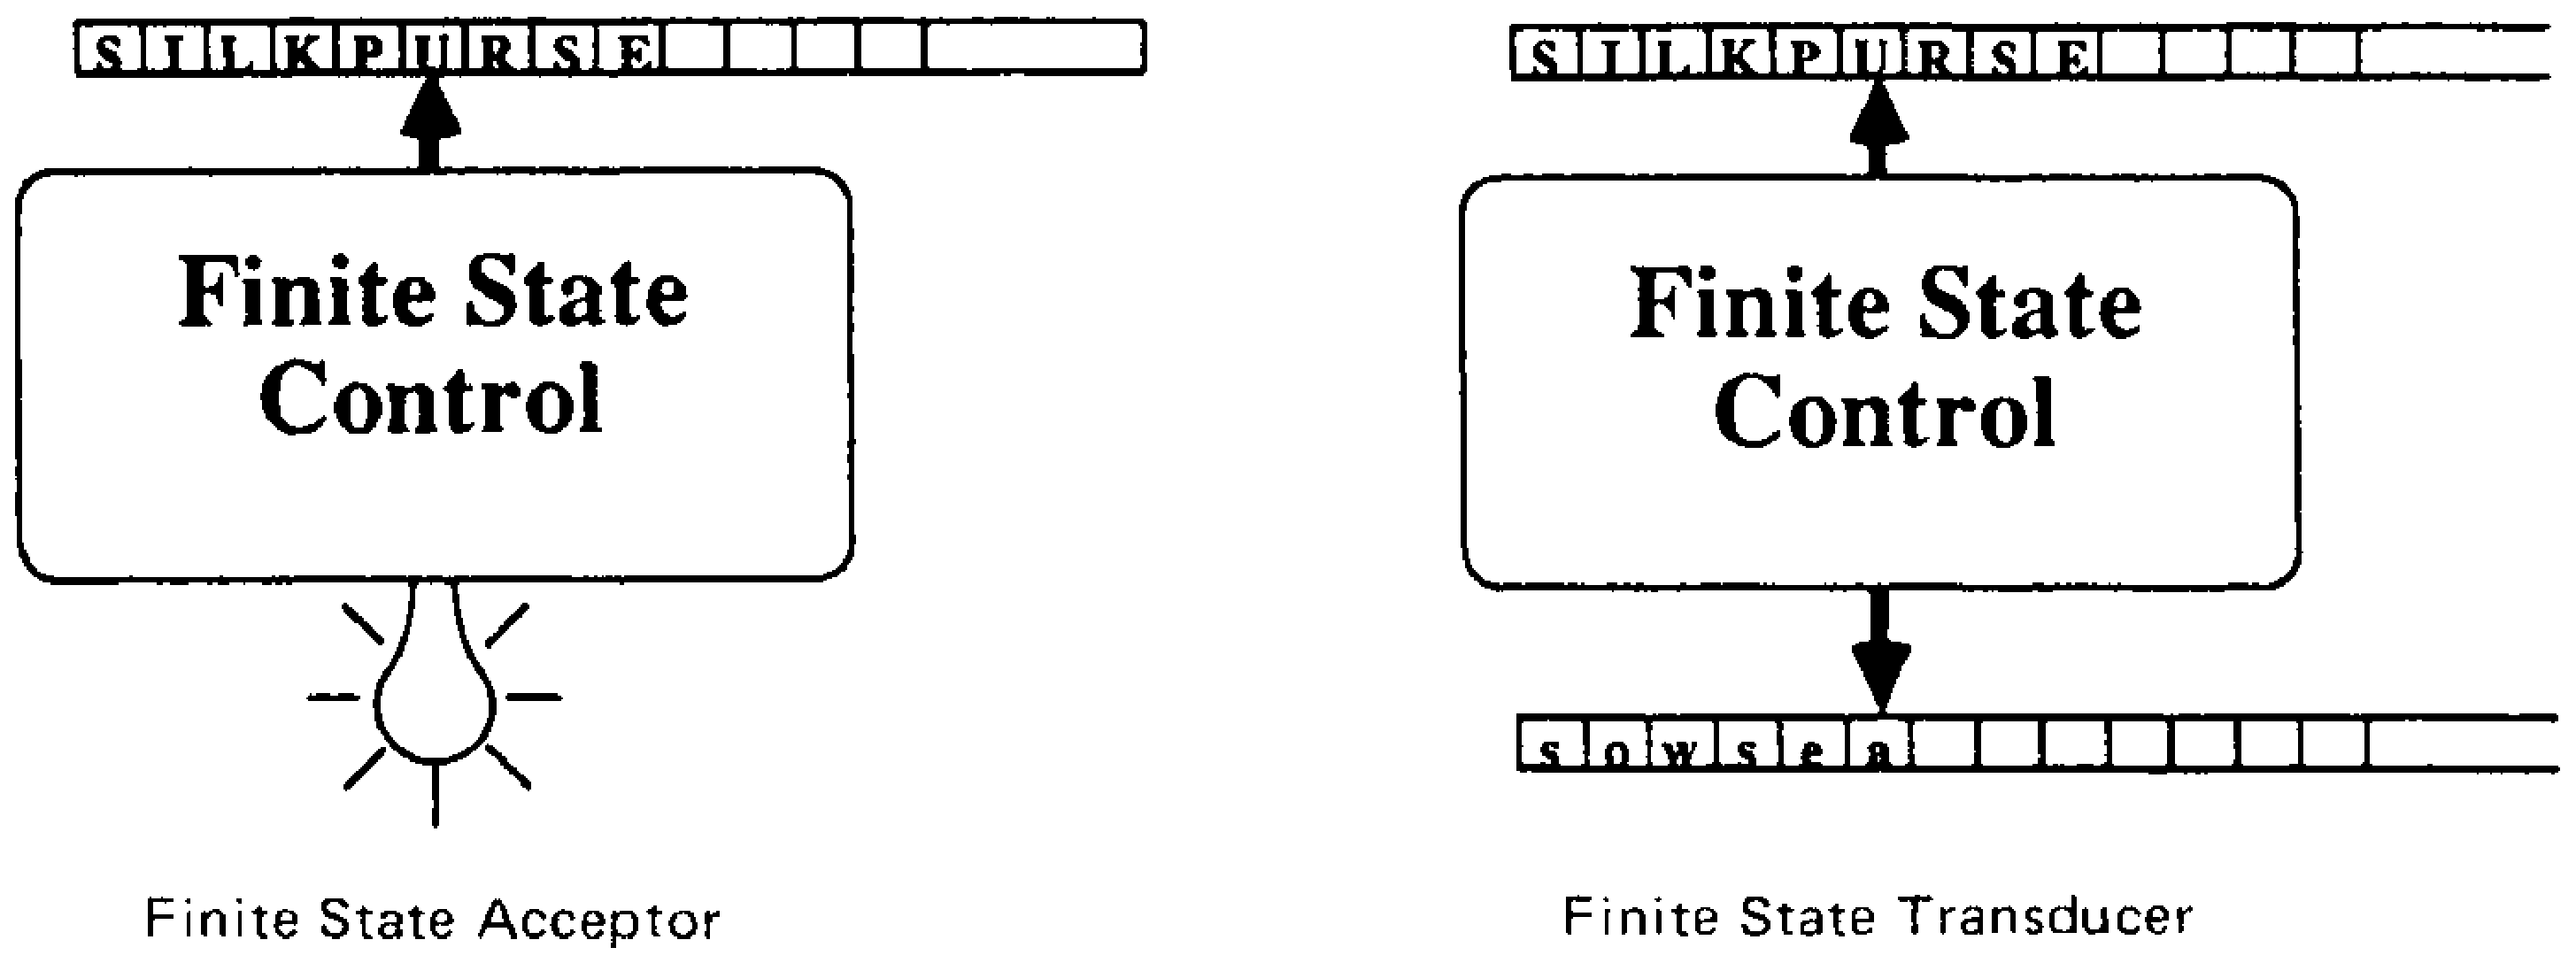
\epsfig{figure=ToFAfigures/fig7-1.eps,width=6in}}
\caption{The difference between an acceptor and a transducer}\label{fig-7.1}
\end{figure}

Also essential to our model is a rule that governs what characters are printed.
For our first type of transducer, this rule will depend on both the current
internal state of the machine and the current symbol being scanned by the read
head and will be represented by the function $\omega$. Finally, since we are
dealing with translation rather than acceptance/rejection, there is no need to
single out accepting states: the concept of final states can be dispensed with
entirely.

\section{Basic Definitions}\label{sec-7.1}

% Definition 7.1
\begin{dfn}\label{dfn-7.1}\index{alphabet!input}\index{alphabet!output}{\index{finite-state transducer|see{FST}}}\index{output alphabet}\index{state transition function!for FST}
A \emph{finite-state transducer} (\Index{FST}) or
\emph{Mealy sequential machine}\index{Mealy sequential machine|see{FST}}
with a distinguished start state is a sextuple
$\langle\Sigma,\Gamma,S,s_0,\delta,\omega\rangle$, where:
\begin{enumerate}[i.]
\item $\Sigma$ denotes the input alphabet.
\item $\Gamma$ denotes the output alphabet.
\item $S$ denotes the set of states, a finite nonempty set.
\item $s_0$ denotes the \emph{\Index{start state}}; $s_0 \in S$.
\item $\delta$ denotes the state transition function; $\delta$$: S \times \Sigma
	\rightarrow S$.
\item $\omega$ denotes the output function; $\omega$$: S \times \Sigma \rightarrow
	\Gamma$.
\end{enumerate}
\end{dfn}

The familiar state transition diagram needs to be slightly modified to represent
these new types of machines. Since there is one labeled arrow for each ordered
pair in the domain of the state transition function and there is also one output
symbol for each ordered pair, we will place the appropriate output symbol by its
corresponding arrow, and separate it from the associated input symbol by a
slash, /.

\subsection*{Example 7.1}

Let $V=\langle\{\pmb{n},\pmb{d},\pmb{q},\pmb{b}\},\{\pmb{\varphi},\pmb{n'},
\pmb{d'},\pmb{q'},\pmb{c}_0,\pmb{c}_1,\pmb{c}_2,\pmb{c}_3,\pmb{c}_4\},S,s_0,
\delta,\omega\rangle$ be the FST illustrated in Figure \ref{fig-7.2}. $V$ describes the
action of a candy machine that dispenses 30\cent\  Chocolate Explosions. $\pmb{n},
\ \pmb{d},\ \pmb{q}$ denote inputs of nickels, dimes, and quarters
(respectively), and $\pmb{b}$ denotes the act of pushing the button to select a
candy bar. $\pmb{\varphi},\pmb{n'},\pmb{d'},\pmb{q'},\pmb{c}_0,\pmb{c}_2,
\pmb{c}_2,\pmb{c}_3,\pmb{c}_4$ represent the vending machine's response to these
inputs: it may do nothing, return the nickel that was just inserted, return the
dime, return the quarter, or dispense a candy bar with 0, 1, 2, 3, or 4 nickels
as change, respectively. Note that the transitions agree with the vending
machine model presented in Chapter \ref{ch-1}; the new model now specifies the action
corresponding to the given input. It is relatively simple to modify the above
machine to include a new input $r$ that signifies that the coin return has been
activated and a new output a representing the release of all coins that have
been inserted (see the exercises).\index{vending machine!FST}

% Figure 7.2
\begin{figure}
\centerline{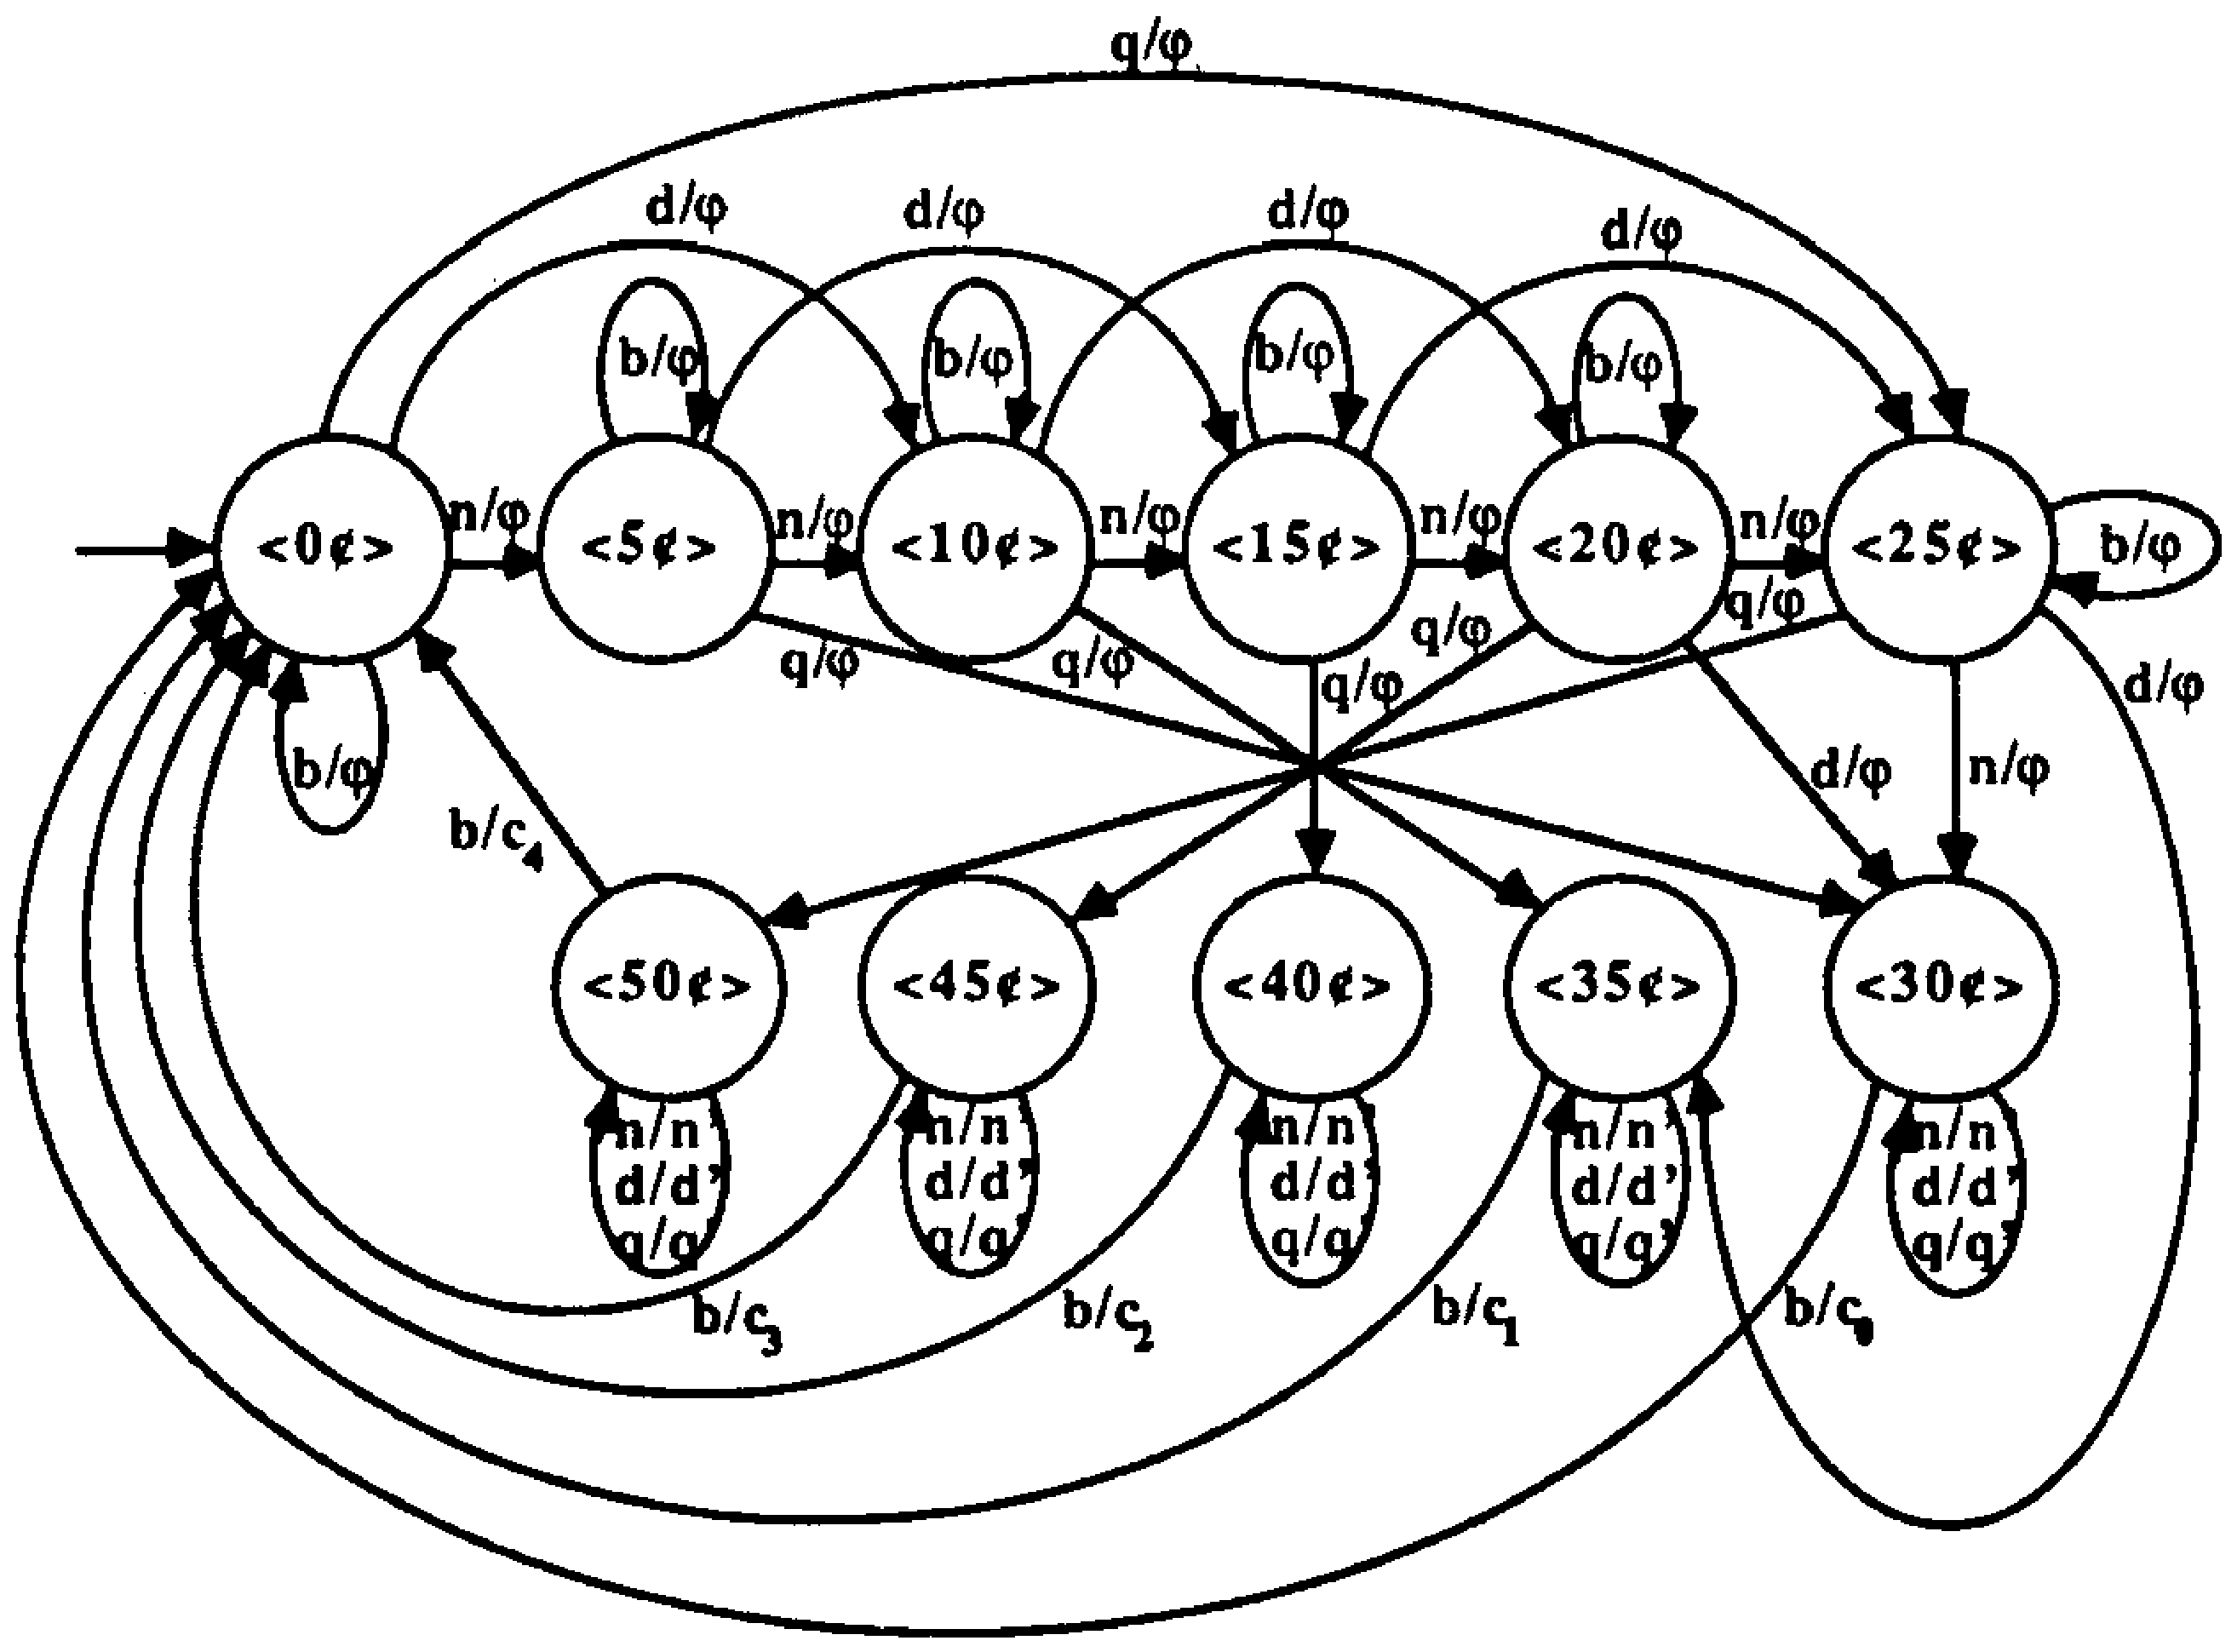
\epsfig{figure=ToFAfigures/fig7-2.eps,width=5.2in}}
\caption{A finite-state transducer model of the vending machine discussed in
Example 7.1}\label{fig-7.2}
\end{figure}

Various modern appliances can be modeled by FSTs. Many microwave ovens accept
input through the door latch mechanism and an array of keypad sensors, and
typical outputs include the control lines to the microwave generator, the
elements of a digital display, an interior light, and an audible buzzer. The
physical circuitry needed to implement these common machines will be discussed
in a later section. We now examine the ramifications of Definition \ref{dfn-7.1} by
concentrating on the details of a very simple finite-state transducer.

\subsection*{Example 7.2}

Let $B=\langle\Sigma,\Gamma,S,s_0,\delta,\omega\rangle$ be given by
\begin{center}
\begin{tabular}{l}
$\Sigma =\{\pmb{a},\pmb{b}\}$ \\
$\Gamma=\{\pmb{0},\pmb{1}\}$ \\
$S = \{s_0,s_1\}$ \\
$s_0 = s_0$
\end{tabular}
\end{center}
The state transition function is defined in Table 7.1a.

% Table 7.1a
% Tables are hand titled due to subnumbering.
\begin{table}[h]\label{tbl-7.1a}
\begin{center}
\begin{tabular}{c|cc}
\multicolumn{3}{c}{Table 7.1a} \\
$\delta$ & $\pmb{a}$ & $\pmb{b}$ \\
\hline
$s_0$ & $s_0$ & $s_1$ \\
$s_1$ & $s_0$ & $s_1$ \\
\end{tabular}
\end{center}
\end{table}
It can be more succinctly specified by ($\forall s \in S)[\delta(s,\pmb{a}) =
s_0$ and $\delta(s,\pmb{b}) = s_1]$. Finally, Table 7.1b displays the
output function, which can be summarized by
$ (\forall c \in \Sigma)[\omega(s_0,c)=0\quad\text{and}\quad\omega(s_1,c) =
	\pmb{1}] $
% Table 7.1b
\begin{table}[h]\label{tbl-7.1b}
\begin{center}\begin{tabular}{c|cc}
\multicolumn{3}{c}{Table 7.1b} \\
$\omega$ & $\pmb{a}$ & $\pmb{b}$ \\
\hline
$s_0$ & $\pmb{0}$ & $\pmb{0}$ \\
$s_1$ & $\pmb{1}$ & $\pmb{1}$
\end{tabular}\end{center}
\end{table}

All the information about $B$ is contained in the diagram displayed in Figure
\ref{fig-7.3}. Consider the input sequence $z=\pmb{abaabbaa}$. From $s_0$, the first
letter of $z$, that is, $\pmb{a}$, causes a $\pmb{0}$ to be printed, since
$\omega(s_0,\pmb{a}) = \pmb{0}$, and since $\delta(s_0,\pmb{a}) = s_0$, the
machine remains in state $s_0$. The second letter $\pmb{b}$ causes a second
$\pmb{0}$ to be printed since $\omega(s_0,\pmb{b}) =\pmb{0}$, but the machine
now switches to state $s_1\ [\delta(s_0,\pmb{b}) = s_1]$. The third input letter
causes a $\pmb{1}$ to be printed $[\omega(s_1,\pmb{a})=\pmb{1}]$, and so on. The
entire output string will be $\pmb{00100110}$, and the machine, after starting
in state $s_0$, will successively assume the state $s_0,s_1,s_0,s_0,s_1,s_1,s_0,
s_0$ as the input string is processed. We are not currently interested in the
terminating state for a given string ($s_0$ in this case), but rather in the
resulting output string, $\pmb{00100110}$.

% Figure 7.3
\begin{figure}
\centerline{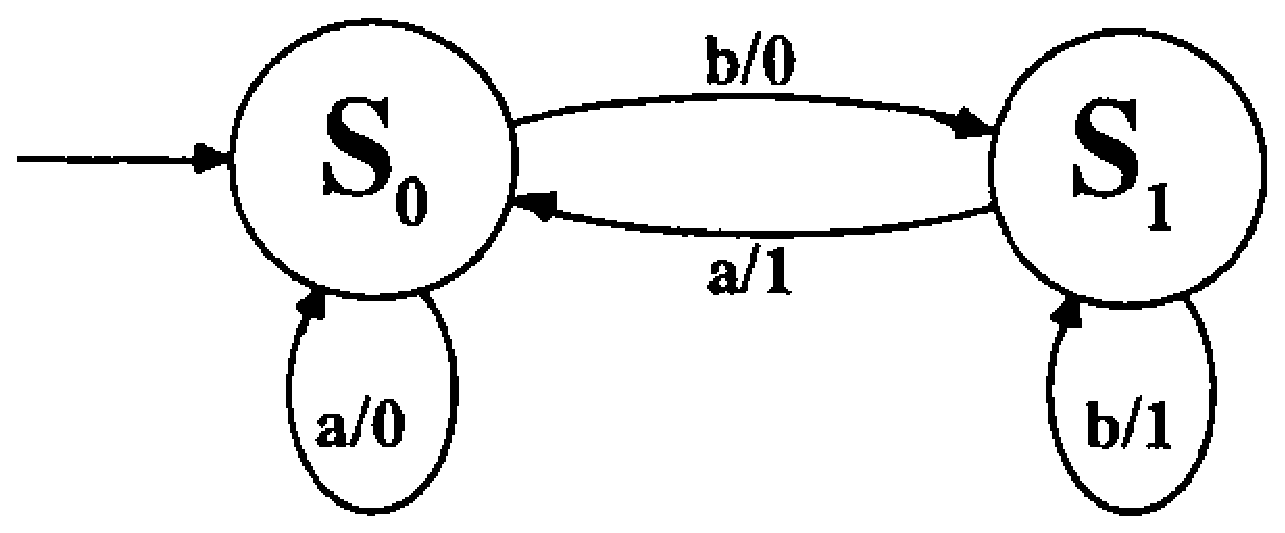
\epsfig{figure=ToFAfigures/fig7-3.eps,width=2in}}
\caption{The state transition diagram for the transducer discussed in Example
7.2}\label{fig-7.3}
\end{figure}

It should be clear that the above discussion illustrates a very awkward way of
describing translations. While $\omega$ describes the way in which single
\emph{letters} are translated, the study of finite-state transducers will
involve descriptions of how entire \emph{strings} are translated. This situation
is reminiscent of the modification of the state transition function $\delta$,
which likewise operated on single letters, to the extended state transition
function $\DBAR$ (which was defined for \emph{strings}). Indeed, what is called
for is an extension of $\omega$ to \OBAR, which will encompass the translation
of entire strings. The translation cited in the last example could then be
succinctly stated as $\OBAR(s_0,\pmb{abaabbaa})=\pmb{00100110}$. That is, the
notation $\OBAR(t,y)$ is intended to represent the output string produced by a
transducer (beginning from state $t$) in response to the input string $y$.

The formal recursive definition of \OBAR\ will depend not only on $\omega$ but
also on the state transition function $\delta$ (and its extension \DBAR).
$\delta$ retains the same conceptual meaning it had for finite-state acceptors:
$\DBAR(s,x)$ denotes the state reached when starting from $s$ and processing, in
sequence, the individual letters of the string $x$. Furthermore, the conclusion
stated in Theorem \ref{thm-1.1} still holds:
\[ (\forall x \in \Sigma^*)(\forall y \in \Sigma^*)(\forall s \in S)(\DBAR(s,yx)
	=\DBAR(\DBAR(s,y),x)) \]
A similar statement can be made about $\omega$ once it has been rigorously
defined.

% Definition 7.2
\begin{dfn}\label{dfn-7.2}\index{extended state transition function \DBAR\! for FST}\index{extended output function \OBAR\! for FST}
Given a FST $A=\langle\Sigma,\Gamma,S,s_0,\delta,\omega\rangle$, the extended
output function for $A$, denoted by \OBAR, is a function $\OBAR$$: S \times
\Sigma^* \rightarrow \Gamma^*$ defined recursively as follows:
\begin{enumerate}[i. ]
% handspaced vs. hardcoding i., ii.
\item $(\forall t \in S)\qquad\qquad\qquad\qquad\ \ \ \thinspace\thinspace\OBAR
	(t,\lambda)=\lambda$
\item $(\forall t \in S)(\forall x \in \Sigma^*)(\forall a \in \Sigma)
	(\OBAR(t,\pmb{a}x)=\omega(t,\pmb{a})\cdot\OBAR(\delta(t,\pmb{a}),x))$
\end{enumerate}
\end{dfn}

\subsection*{Example 7.3}

Let $B=\langle\Sigma,\Gamma,S,s_0,\delta,\omega\rangle$ be the FST given in
Example 7.2. Then
\begin{center}
\begin{tabular}{rl}
$\OBAR(s_1,\pmb{baa})$ & $=\omega(s_1,\pmb{b}) \cdot \OBAR(\delta(s_1,\pmb{b}),
	\pmb{aa}) = \pmb{1} \cdot \OBAR(s_1,\pmb{aa})$ \\
& $= \pmb{1} \cdot \omega(s_1,\pmb{a})\cdot\OBAR(\delta(s_1,\pmb{a}),\pmb{a}) =
	\pmb{11}\cdot \OBAR(s_0,\pmb{a}) = \pmb{110}$
\end{tabular}
\end{center}
Note that a three-letter input sequence gives rise to exactly three output
symbols: $\OBAR$ is \emph{\Index{length preserving}}, in the sense that
$(\forall t \in S)(\forall x \in \Sigma^*)(|\OBAR(t,x)| = |x|)$.

The \OBAR\ function extends the $\omega$ function from single letters to words.
Whereas the $\omega$ function maps a state and a \emph{letter} to a single
symbol from $\Gamma$, the \OBAR\ function maps a state and a \emph{word} to an
entire \emph{string} from $\Gamma^*$. It can be deduced from (i) and (ii) (see
the exercises) that (iii) ($\forall t \in S)(\forall a \in \Sigma)(\OBAR(t, a)
= \omega(t,a))$, which is the observation that $\omega$ and \OBAR\ treat single
letters the same. The extended output function \OBAR\ has properties similar to
those of \DBAR, in that the single letter $\pmb{a}$ found in the recursive
definition of \OBAR\ can be replaced by an entire word $y$. The analog of
Theorem \ref{thm-1.1} is given below.

% Theorem 7.1
\begin{thm}\label{thm-7.1}
Let $A=\langle\Sigma,\Gamma,S,s_0,\delta,\omega\rangle$ be a FST. Then:
\[ (\forall x \in \Sigma^*)(\forall y \in \Sigma^*)(\forall t \in S)(\OBAR(t,yx)
	= \OBAR(t,y) \cdot \OBAR(\DBAR(t,y),x)) \]
and
\[ (\forall x \in \Sigma^*)(\forall y \in \Sigma^*)(\forall s \in S)(\DBAR(s,yx)
	= \DBAR(\DBAR(s,y),x)) \]

\emph{Proof.} The proof is by induction on $|y|$ (see the exercises and compare
with Theorem \ref{thm-1.1}).
\end{thm}

\subsection*{Example 7.4}

Let $B=\langle\Sigma,\Gamma,S,s_0,\delta,\omega\rangle$ be the FST given in
Example 7.2. Consider the string $z=\pmb{abaabbaa}=yx$, where $y=\pmb{abaab}$
and $x=\pmb{baa}$. To apply Theorem \ref{thm-7.1} with $t=s_0$, we first calculate
$\OBAR(s_0,y) = \OBAR(s_0,\pmb{abaab}) = \pmb{00100}$, and $\DBAR(s_0,y) = s_1$.
From Example 7.3, $\OBAR(s_1,\pmb{baa}) = \pmb{110}$, and hence, as required by
Theorem \ref{thm-7.1},
\[ \pmb{00100110} = \OBAR(s_0,\pmb{abaabbaa}) = \OBAR(s_0,yx) = \OBAR(s_0,y)
	\cdot \OBAR(\DBAR(s_0,y),x) = \pmb{00100} \cdot \pmb{110} \]

For a given FST $A$ with a specified start state, the deterministic nature of
finite-state transducers requires that each input string be translated into a
\emph{unique} output string; that is, the relation $f_A$ that associates input
strings with their corresponding output strings is a \emph{function}.

% Definition 7.3
\begin{dfn}\label{dfn-7.3}{\index{translation function!FST}}
Given a FST $M=\langle\Sigma,\Gamma,S,s_0,\delta,\omega\rangle$, the
\emph{translation function} for $M$, denoted by $f_M$, is the function
$f_M$$: \Sigma^* \rightarrow \Gamma^*$ defined by $f_M(x) = \OBAR(s_0,x)$.
\end{dfn}

Note that $f_M$, like \OBAR, is \emph{length preserving}:
$(\forall x \in \Sigma^*)(|f_M(x)| = |x|)$. Consequently, for any $n \in \NN$,
if the domain of $f_M$ were restricted to $\Sigma^n$, then the range of $f_M$
would likewise be contained in $\Gamma^n$.

\subsection*{Example 7.5}

Let $B=\langle\Sigma,\Gamma,S,s_0,\delta,\omega\rangle$ be the finite-state
transducer given in Figure \ref{fig-7.3}. Since $\OBAR(s_0,\pmb{abaab})=(\pmb{00100})$,
$f_B(\pmb{abaab}) = \pmb{00100}$. Similarly, $f_B(\lambda) = \lambda$,
$f_B(\pmb{a})=\pmb{0}$, $f_B(\pmb{b})=\pmb{0}$, $f_B(\pmb{aa})=\pmb{00}$,
$f_B(\pmb{ab})=\pmb{00}$, $f_B(\pmb{ba})=\pmb{01}$, $f_B(\pmb{bb})=\pmb{01}$.
Coupled with these seven base definitions, this particular $f_B$ could be
recursively defined by
\begin{align*}
(\forall x \in \Sigma^*)f_B(x\pmb{aa}) = f_B(x\pmb{a}) \cdot \pmb{0} \\
f_B(x\pmb{ab}) = f_B(x\pmb{a}) \cdot \pmb{0} \\
f_B(x\pmb{ba}) = f_B(x\pmb{b}) \cdot \pmb{1}
\intertext{and}f_B(x\pmb{bb}) = f_B(x\pmb{b}) \cdot \pmb{1}
\end{align*}
$f_B$ in essence replaces $\pmb{a}$s with $\pmb{0}$s and $\pmb{b}$s with $\pmb{1}$s,
and ``delays'' the output by one letter. More specifically, the translation
function for $B$ takes an entire string and substitutes $\pmb{0}$s and
$\pmb{1}$s for $\pmb{a}$s and $\pmb{b}$s (respectively), deletes the last letter of
the string, and appends a $\pmb{0}$ to the front of the resulting string. The
purpose of the two states $s_0$ and $s_1$ in the FST $B$ is to remember whether
the previous symbol was an $\pmb{a}$ or a $\pmb{b}$ (respectively) and output the
appropriate replacement letter. Note that $\pmb{1}$s are always printed on
transitions from $s_1$, and $\pmb{0}$s are printed as we leave $s_0$.

\subsection*{Example 7.6}

Let $C=\langle\{\pmb{a},\pmb{b}\},\{\pmb{0},\pmb{1}\},\{t_0,t_1,t_2,t_3\},t_0,
\delta_C,\omega_C\rangle$ be the FST shown in Figure \ref{fig-7.4}. $C$ \emph{flags}
occurrences of the string $\pmb{aab}$ by printing a $\pmb{1}$ on the output tape
\index{tape!output} only when the substring $\pmb{aab}$ appears in the input stream.

% Figure 7.4
\begin{figure}
\centerline{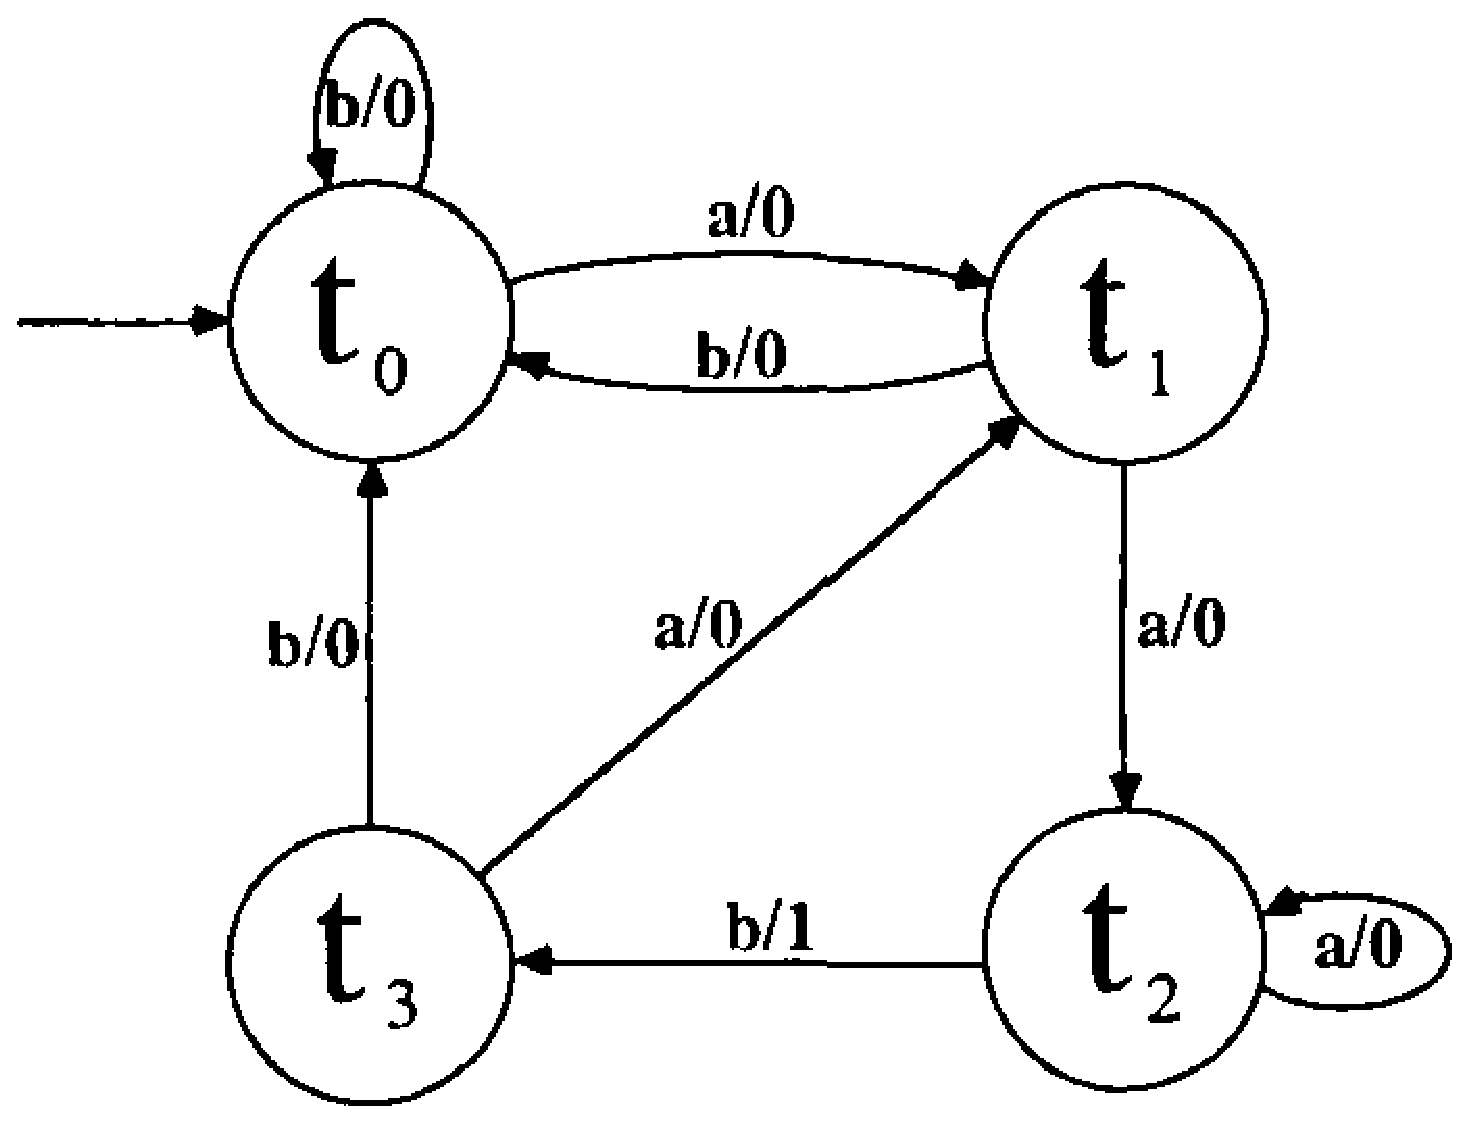
\epsfig{figure=ToFAfigures/fig7-4.eps,width=2.5in}}
\caption{The state transition diagram for the Mealy machine $C$ in
Example 7.6}\label{fig-7.4}
\end{figure}

Clearly, not all functions from $\Sigma^*$ to $\Gamma^*$ can be represented by
finite-state transducers; we have already observed that functions that are not
length preserving cannot possibly qualify. As the function discussed later in
Example 7.7 shows, not all length-preserving functions qualify, either.

% Definition 7.4
\begin{dfn}\label{dfn-7.4}
Given a function $f$$: \Sigma^* \rightarrow \Gamma^*,\ f$ is \emph{finite transducer definable}\index{finite
transducer definable|see{FTD}} (\Index{FTD}) iff there exists a transducer $A$ such
that $f=f_A$.
\end{dfn}

Due to the deterministic nature of transducers, any two strings that ``begin
the same'' must start being ``translated the same.'' This observation is the
basis for the following theorem.

% Theorem 7.2
\begin{thm}\label{thm-7.2}
Assume $f$ is FTD. Then

%\begin{tabular}{l}
$(\forall n \in \NN)(\forall x \in \Sigma^n)(\forall y \in \Sigma^*)
	(\forall z \in \Sigma^*)(\text{the first }n\text{ letters of }f(xy)$ 
	must agree with the first $n$ letters of $f(xz))$
%\end{tabular}

\emph{Proof.} See the exercises.
\end{thm}

\subsection*{Example 7.7}

Consider the function $g$$:\{\pmb{a},\pmb{b},\pmb{c}\}^* \rightarrow
\{\pmb{0},\pmb{1}\}^*$, which replaces input symbols by $\pmb{0}$ unless the
next letter is $\pmb{c}$, in which case $\pmb{1}$ is used instead. Thus,
\[ g(\pmb{abcaaccb}) = \pmb{01001100}\text{ and }g(\pmb{abb}) = \pmb{000}. \]
With $n = 2$, choosing $x = \pmb{ab}$, $y = \pmb{caaccb}$, and $z = \pmb{b}$
shows that $g$ violates Theorem \ref{thm-7.2}, so $g$ cannot be FTD.

The necessary condition outlined in the previous theorem is by no means
sufficient to guarantee that a function is FTD; other properties such as a
pumping lemma-style repetitiousness of the translation must also be present (see
the exercises).

\section{Minimization of Finite-State Transducers}\label{sec-7.2}

Two transducers that perform exactly the same translation over the entire range
of input strings from $\Sigma$ will be called \emph{equivalent} transducers.
This is in spirit similar to the way equivalence was defined for deterministic
finite automata.

% Definition 7.5
\begin{dfn}\label{dfn-7.5}\index{equivalent!transducers}
Given transducers
\[ A=\langle\Sigma,\Gamma,S_A,s_{0_A},\delta_A,\omega_A\rangle\quad\text{and}
	\quad B=\langle\Sigma,\Gamma,S_B,s_{0_B},\delta_B,\omega_B\rangle, \]
$A$ is said to be \emph{equivalent} to $B$ iff $f_A = f_B$.
\end{dfn}

Just as with finite automata, a reasonable goal when constructing a transducer
is to produce an efficient machine, and, as before, this will be equated with
the size of the finite-state control; given a translation function $f$, a
minimal machine for $f$ is a FST that has the minimum number of states necessary
to perform the required translation.

% Definition 7.6
\begin{dfn}\label{dfn-7.6}
Given a finite-state transducer
$A=\langle\Sigma,\Gamma,S_A,s_{0_A},\delta_A,\omega_A\rangle$, $A$ is the
\emph{\Index{minimal Mealy machine} for the translation} $f_A$ iff for all
finite-state transducers
$B=\langle\Sigma,\Gamma,S_B,s_{0_B},\delta_B,\omega_B\rangle$ for which
$f_A = f_B,\ \|S_A\| \leq \|S_B\|$.
\end{dfn}

Thus, $A$ is minimal if there is no equivalent machine with fewer states.

\subsection*{Example 7.8}

The FST $C=\langle\{\pmb{a},\pmb{b}\},\{\pmb{0},\pmb{1}\},\{t_0,t_1,t_2,t_3\},
t_0,\delta_C,\omega_C\rangle$ given in Figure \ref{fig-7.4} is \emph{not} minimal. The FST
$D=$\linebreak$\langle\{\pmb{a},\pmb{b}\},\{\pmb{0},\pmb{1}\},\{q_0,q_1,q_2\},q_0,\delta_D,
\omega_D\rangle$ given in Figure \ref{fig-7.5} performs the same translation, but has only
three states.\index{equivalent!transducers}

% Figure 7.5
\begin{figure}
\centerline{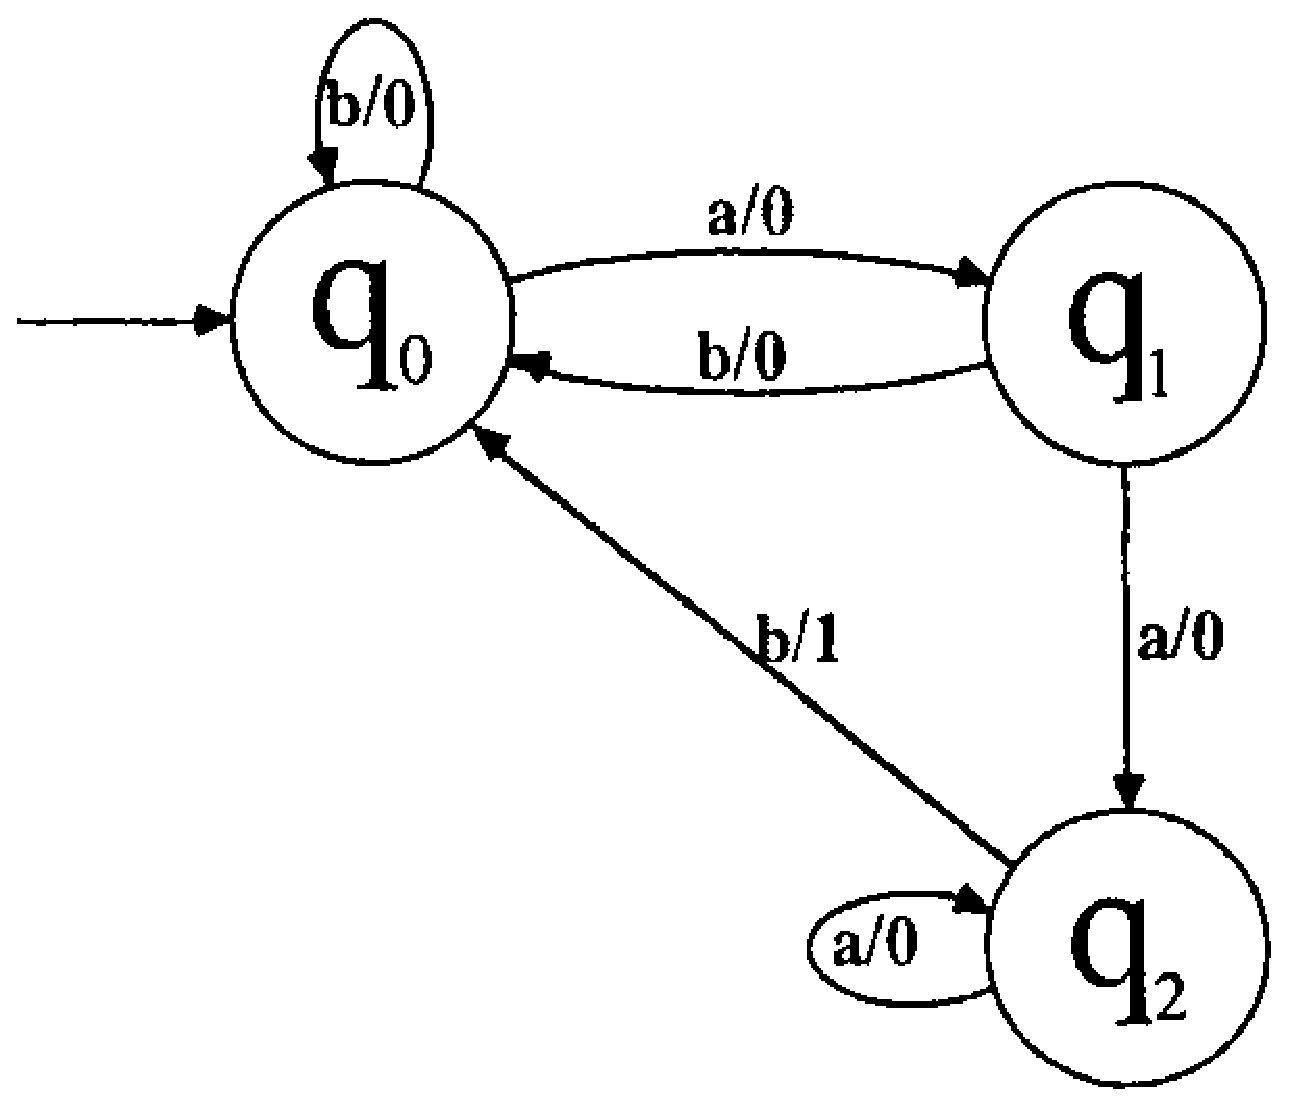
\epsfig{figure=ToFAfigures/fig7-5.eps,width=2.5in}}
\caption{The state transition diagram for the Mealy machine $D$ in Example 7.8}\label{fig-7.5}
\end{figure}

The concept of two transducers being essentially the same except for a trivial
renaming of the states will again be formalized through the definition of
\emph{isomorphism}\index{isomorphism!between FSTs} (and
\emph{homomorphism}).\index{homomorphism!between FSTs} As before, it will
be important to match the respective start states and state transitions; but
rather than matching up final states (which do not exist in the FST model), we
must instead ensure that the output function is preserved by the relabeling
process.

% Definition 7.7
\begin{dfn}\label{dfn-7.7}
Given two FSTs
\[ A=\langle\Sigma,\Gamma,S_A,s_{0_A},\delta_A,\omega_A\rangle\quad\text{and}
	\quad B=\langle\Sigma,\Gamma,S_B,s_{0_B},\delta_B,\omega_B\rangle, \]
and a function $\mu$$: S_A \rightarrow S_B,\ \mu$ is called a \emph{\Index{Mealy
machine homomorphism}} from $A$ to $B$ iff the following three conditions hold:
\begin{enumerate}[i.]
\item $\mu(s_{0_A}) = s_{0_B}$.
\item $(\forall s \in S_A)(\forall\pmb{a} \in \Sigma)(\mu(\delta_A(s,\pmb{a}))
	= \delta_B(\mu(s),\pmb{a}))$.
\item $(\forall s \in S_A)(\forall\pmb{a} \in \Sigma)(\omega_A(s,\pmb{a}) =
	\omega_B(\mu(s),\pmb{a}))$.
\end{enumerate}
\end{dfn}

As in Chapter \ref{ch-3}, a bijective homomorphism will be called an isomorphism and will
signify that the isomorphic machines are essentially the same (except perhaps
for the names of the states). The isomorphism is essentially a recipe for
renaming the states of one machine to produce identical transducers.

% Definition 7.8
\begin{dfn}\label{dfn-7.8}
Given two FSTs
\[ A=\langle\Sigma,\Gamma,S_A,s_{0_A},\delta_A,\omega_A\rangle\quad\text{and}
	\quad B=\langle\Sigma,\Gamma,S_B,s_{0_B},\delta_B,\omega_B\rangle, \]
and a function $\mu$$: S_A \rightarrow S_B,\ \mu$ is called a \emph{\Index{Mealy
machine isomorphism}} from $A$ to $B$ iff the following five conditions hold:
\begin{enumerate}[i.]
\item $\mu(s_{0_A}) = s_{0_B}$.
\item $(\forall s \in S_A)(\forall\pmb{a} \in \Sigma)(\mu(\delta_A(s,\pmb{a}))
	= \delta_B(\mu(s),\pmb{a}))$.
\item $(\forall s \in S_A)(\forall\pmb{a} \in \Sigma)(\omega_A(s,\pmb{a}) =
	\omega_B(\mu(s),\pmb{a}))$.
\item $\mu$ is a one-to-one function from $S_A$ to $S_B$.
\item $\mu$ is onto $S_B$.
\end{enumerate}
\end{dfn}

% Definition 7.9
\begin{dfn}\label{dfn-7.9}
If $\mu$$: S_A \rightarrow S_B$ is an isomorphism between two transducers
$A=\langle\Sigma,\Gamma,S_A,s_{0_A},\delta_A,\omega_A\rangle$ and
$B=\langle\Sigma,\Gamma,S_B,s_{0_B},\delta_B,\omega_B\rangle$, then $A$ is said
to be \emph{\Index{isomorphic}} to $B$, and we will write $A \cong B$.
\end{dfn}

\subsection*{Example 7.9}

Consider the two FSTs
$C=\langle\{\pmb{a},\pmb{b}\},\{\pmb{0},\pmb{1}\},\{t_0,t_1,t_2,t_3\},t_0,
\delta_C,\omega_C\rangle$, given in Figure \ref{fig-7.4}, and
$D=$\linebreak$\langle\{\pmb{a},\pmb{b}\},\{\pmb{0},\pmb{1}\},\{q_0,q_1,q_2\},q_0,\delta_D,
\omega_D\rangle$, displayed in Figure \ref{fig-7.5}. The function $u$$:\{t_0,t_1,t_2,t_3\} 
\rightarrow\{q_0,q_1,q_2\}$, defined by $\mu(t_0)=q_0,\ \mu(t_1)=q_1,\ 
\mu(t_2)=q_2$, and $\mu(t_3)=q_0$ is a homomorphism between C and D. Conditions
(i) and (ii) are exactly the same criteria used for finite automata
homomorphisms and have exactly the same interpretation: the start states must
correspond and the transitions must match. The third condition is present to
ensure that the properties of the $\omega$ function are respected; for example,
since $t_2$ causes $\pmb{1}$ to be printed when $\pmb{b}$ is processed, so should
the corresponding state in the $D$ machine, which is $q_2=\mu(t_2)$ in this
example. Indeed, $\omega_C(t_2,\pmb{b})=\pmb{1}=\omega_D(\mu(t_2),\pmb{b})$.
Such similarities extend to full strings also: note that $\OBAR_C(t_0,\pmb{aab})
=\pmb{001}=\OBAR_D(\mu(t_0),\pmb{aab})$ in this example. The results can be
generalized as presented in the next lemma.

% Lemma 7.1
\begin{lmm}\label{lmm-7.1}
If $\mu$$: S_A \rightarrow S_B$ is a homomorphism between two FSTs
\[ A=\langle\Sigma,\Gamma,S_A,s_{0_A},\delta_A,\omega_A\rangle\text{ and }
	B=\langle\Sigma,\Gamma,S_B,s_{0_B},\delta_B,\omega_B\rangle, \]
then
\[ (\forall s \in S_A)(\forall x \in \Sigma^*)(\mu(\DBAR_A(s,x)) = 
	\DBAR_B(\mu(s),x)) \]
and
\[ (\forall s \in S_A)(\forall x \in \Sigma^*)(\OBAR_A(s,x) =
	\OBAR_B(\mu(s),x)) \]
\emph{Proof.} The proof is by induction on $|x|$ (see the exercises).
\end{lmm}

% Corollary 7.1
\begin{cor}\label{cor-7.1}
If $\mu$$: S_A \rightarrow S_B$ is a homomorphism between two FSTs
$A=\langle\Sigma,\Gamma,S_A,s_{0_A},\delta_A,\omega_A\rangle$ and
$B=\langle\Sigma,\Gamma,S_B,s_{0_B},\delta_B,\omega_B\rangle$, then $A$ is
equivalent to $B$; that is, $f_A = f_B$.

\emph{Proof.} The proof follows immediately from Lemma \ref{lmm-7.1} and the definition of
$f_M$.
\end{cor}

In a manner very reminiscent of the approach taken to minimize deterministic
finite automata, notions of state equivalence relations, reduced machines, and
connectedness can be defined. As was the case in Chapter \ref{ch-3}, a reduced and
connected machine will be isomorphic to every other equivalent minimal machine.
The definition for connectedness is essentially unchanged.

% Definition 7.10
\begin{dfn}\label{dfn-7.10}\index{accessible state}\index{A@$A^c$ (A connected)!for FST}
A state $s$ in a transducer $M=\langle\Sigma,\Gamma,S,s_0,\delta,\omega\rangle$
is called \emph{accessible} iff
\[ (\exists x_s \in \Sigma^*) \ni \DBAR(s_0,x_s) = s \]
The transducer $M=\langle\Sigma,\Gamma,S,s_0,\delta,\omega\rangle$ is called
\emph{connected} iff
\[ (\forall s \in S)(\exists x_s \in \Sigma^*) \ni \DBAR(s_0,x_s) = s \]
\end{dfn}

That is, every state $s$ of $S$ can be reached by some string ($x_s$) in
$\Sigma^*$; once again, the choice of the state $s$ will have a bearing on which
particular string is used as a representative. States that are not accessible do
not affect the translation performed by the transducer; such states can be
safely deleted to form a connected version of the machine.

% Definition 7.11
\begin{dfn}\label{dfn-7.11}\index{M connected (FST $M^c$)}
Given a FST $M=\langle\Sigma,\Gamma,S,s_0,\delta,\omega\rangle$, define the
transducer $M^c=\langle\Sigma,\Gamma,S^c,s^c_0,\delta^c,\omega^c\rangle$, called
\emph{$M$ connected}, by
\begin{center}\begin{tabular}{l}
$S^c=\{s \in S$ $|$ $\exists x \in \Sigma^* \ni \DBAR(s_0,x) = s\}$ \\
$s^c_0 = s_0$
\end{tabular}\end{center}
$\delta^c$ is essentially the restriction of $B$ to $S^c\!\times \Sigma$$:
(\forall\pmb{a}\in\Sigma)(\forall s \in S^c)(\delta^c(s,\pmb{a})=\delta(s,a))$,
and $\omega^c$ is the restriction of $\omega to\ S^c\!\times \Sigma$$:
(\forall\pmb{a}\in\Sigma)(\forall s \in S^c)(\omega^c(s,\pmb{a}) =
\omega(s,\pmb{a}))$.
\end{dfn}

$M^c$ is, as in Chapter \ref{ch-3}, the machine $M$ with the unreachable states ``thrown
away.'' As with DFAs, trimming a machine in this fashion has no effect on the
operation of the transducer. To formally prove this, the following lemma is 
needed.

% Lemma 7.2
\begin{lmm}\label{lmm-7.2}
Given transducers
\[ M=\langle\Sigma,\Gamma,S,s_0,\delta,\omega\rangle\quad\text{and}\quad M^c =
\langle\Sigma,\Gamma,S^c,s^c_0,\delta^c,\omega^c\rangle, \]
the restriction of \  $\overline\omega$ to\ \ $S^c \times \Sigma^*$ is $\overline{\omega^c}$.

\emph{Proof.} We must show that $(\forall y \in \Sigma^*)(\forall t \in S^c)
(\overline{\omega^c}(t,y)=\OBAR(t,y))$. This can be done with a straightforward induction on
$|y|$. Let $P(n)$ be defined by
\[ (\forall y \in \Sigma)(\forall t \in S^c)(\overline{\omega^c}(t,y) = \OBAR(t,y)). \]
The basis step is trivial, since\ \ $\overline{\omega^c}(t,\lambda)=\lambda=\OBAR(t,\lambda)$.
For the inductive step, assume
$(\forall y \in \Sigma^m)(\forall t \in S^c)(\overline{\omega^c}(t,y)=\OBAR(t,y))$, and let
$t \in S^c$ and $z \in \Sigma^{m+1}$ be given. Then $\exists x \in \Sigma^m,\ 
\exists\pmb{a} \in \Sigma$ for which $z = \pmb{a}x$, and therefore
\begin{center}\begin{tabular}{rcl}
$\overline{\omega^c}(t,z)$ & $=$ & (by definition of $z$) \\
$\overline{\omega^c}(t,\pmb{a}x)$ & $=$ & (by Definition \ref{dfn-7.2}ii) \\
$\omega^c(t,\pmb{a})\cdot\overline{\omega^c}(\delta^c(t,\pmb{a}),x)$ & $=$ &
	(by definition of $\delta^c$) \\
$\omega^c(t,\pmb{a})\cdot\overline{\omega^c}(\delta(t,\pmb{a}),x)$ & $=$ &
	(by the induction assumption) \\
$\omega^c(t,\pmb{a})\cdot\OBAR(\delta(t,\pmb{a}),x)$ & $=$ &
	(by definition of $\omega^c$) \\
$\omega(t,\pmb{a})\cdot\OBAR(\delta(t,\pmb{a)},x)$ & $=$ &
	(by Definition \ref{dfn-7.2}ii) \\
$\OBAR(t,\pmb{a}x)$ & $=$ & (by definition of $z$) \\
$\OBAR(t,z)$ &&
\end{tabular}\end{center}
Since $z$ was an arbitrary element of $\Sigma^{m+1}$\!, and $t$ was an arbitrary
state in $S^c$,
\[ (\forall y \in \Sigma^{m+1})(\forall t \in S^c)(\overline{\omega^c}(t,z)=\OBAR(t,z)), \]
which proves $P(m+1)$. Hence, $P(m) \Rightarrow P(m+1)$, and, since $m$ was
arbitrary, $(\forall m \in \NN)(P(m) \Rightarrow P(m+1))$. By the principle of
mathematical induction, $P(n)$ is therefore true for all $n$, and the lemma is
proved.
\end{lmm}

Since $\overline{\omega^c} = \OBAR$, it immediately follows that $f_M = f_{M^c}$, and we are
therefore assured that the operation of any transducer is indistinguishable from
the operation of its connected counterpart.

% Theorem 7.3
\begin{thm}\label{thm-7.3}
Given transducers
\[ M=\langle\Sigma,\Gamma,S,s_0,\delta,\omega\rangle\quad\text{and}\quad
	M^c=\langle\Sigma,\Gamma,S^c,s^c_0,\delta^c,\omega^c\rangle, \]
$M$ is equivalent to $M^c$.

\emph{Proof.} $f_{M^c}(x)=\overline{\omega^c}(s^c_0,x)=\overline{\omega^c}(s_0,x)=\OBAR(s_0,x)=f_M(x)$,
and hence by the definition of equivalence of transducers, $M$ is equivalent to
$M^c$.
\end{thm}

% Corollary 7.2
\begin{cor}\label{cor-7.2}
Given a FTD function $f$, the minimal machine corresponding to $f$ must be
connected.

\emph{Proof.} (by contradiction): Assume the minimal machine $M$ is not
connected; then, by Theorem \ref{thm-7.3}, $f_{M^c} = f_M = f$, and clearly
$\|S^c\| < \|S\|$, and hence $M$ could not be minimal.
\end{cor}

While connectedness is a necessary condition for minimality, it is not
sufficient, as evidenced by the machine $C$ in Figure \ref{fig-7.4}: $C$ was connected,
but the FST $D$ in Figure \ref{fig-7.5} was an equivalent but smaller transducer.

As was the case with finite automata in Chapter \ref{ch-3}, connectedness is just one
of the two major requirements for minimality. The other requirement is that no
two states behave identically. For DFAs, this translated into statements about
acceptance and rejection. For FSTs, this will instead involve the behavior of
the output function. The analog to Definition \ref{dfn-3.2} is given next.

% Definition 7.12
\begin{dfn}\label{dfn-7.12}\index{equivalent!{FST states}}\index{state equivalence relation!for transducers}
Given a transducer $M=\langle\Sigma,\Gamma,S,s_0,\delta,\omega\rangle$, the
\emph{state equivalence relation} on $M$, $E_M$, is defined by
\[ (\forall s \in S)(\forall t \in S)(s E_M t \Leftrightarrow
	(\forall x \in \Sigma^*)(\OBAR(s,x) = \OBAR(t, x))) \]
\end{dfn}

In other words, we will relate states $s$ and $t$ if and only if it is not
possible to determine, by only observing the output, whether we are starting
from state $s$ or state $t$ (no matter what input string is used). The more
efficient machines will not have such duplication of states, and, as with DFAs,
will be said to be \emph{reduced}.

% Definition 7.13
\begin{dfn}\label{dfn-7.13}\index{reduced!FST,MSM}
A transducer $M=\langle\Sigma,\Gamma,S,s_0,\delta,\omega\rangle$ is called
\emph{reduced} iff $(\forall s,t \in S)(s E_M t \Leftrightarrow s = t)$.
\end{dfn}

As before, if $M$ is reduced, $E_M$ must be the identity relation on the set of
states $S$, and each equivalence class must contain only a single element. We
defer for  the moment the discussion of how $E_M$ can be efficiently calculated.
Once the state equivalence relation is known, in a manner that is also analogous
to the treatment of finite automata, states related by $E_M$ can be coalesced to
form a machine that is reduced.

% Definition 7.14
\begin{dfn}\label{dfn-7.14}\index{A @$ A/_{E_A}$ (A modulo $E_A$)!for FST}
Given a FST $M=\langle\Sigma,\Gamma,S,s_0,\delta,\omega\rangle$, define
\emph{$M$ modulo its state equivalence relation}, \Index{M$/\!\!_{E_M}$}, by
$M/\!\!_{E_M}=\langle\Sigma,\Gamma,S_{E_M},s_{0_{E_M}},\delta_{E_M},\omega_{E_M}
\rangle$, where
\begin{center}\begin{tabular}{rcl}
$S_{E_M}$ & $=$ & $\{[s]_{E_M}$ $|$ $s \in S\}$ \\
$s_{0_{E_M}}$ & $=$ & $[s_0]_{E_M}$
\end{tabular}\end{center}
$\delta_{E_M}$ is defined by
\[ (\forall a \in \Sigma)(\forall [s]_{E_M} \in S_{E_M})(\delta_{E_M}([s]_{E_M},
	\pmb{a}) = [\delta(s,\pmb{a})]_{E_M}), \]
and $\omega_{E_M}$ is defined by
\[ (\forall a \in \Sigma)(\forall [s]_{E_M} \in S_{E_M})(\omega_{E_M}([s]_{E_M},
	\pmb{a}) = \omega(s,\pmb{a})). \]
\end{dfn}

The proof that $\delta_{E_M}$ is well defined is similar to that found in
Chapter \ref{ch-3}. In an analogous fashion, $\omega_{E_M}$ must be shown to be well
defined (see the exercises).

All the properties that one would expect of $M/\!\!_{E_M}$ are present, as outlined
in the following theorem.

% Theorem 7.4
\begin{thm}\label{thm-7.4}
Given a FST $M=\langle\Sigma,\Gamma,S,s_0,\delta,\omega\rangle$,
\[ M/\!\!_{E_M}= \langle\Sigma,\Gamma,S_{E_M},s_{0_{E_M}},\delta_{E_M},\
	\omega_{E_M}\rangle \]
is equivalent to $M$ and is reduced. Furthermore, if $M$ is connected, so is
$M/\!\!_{E_M}$

\emph{Proof.} The proof that connectedness is preserved is identical to that
given for Theorem \ref{thm-3.5}; showing that $M/\!\!_{E_M}$ is reduced is very similar to the
proof of Theorem \ref{thm-3.4}. The proof of the fact that the two machines are equivalent
requires the inductive argument that $(\forall y \in \Sigma^*)(\forall t \in S)
(\OBAR(t,y) = \OBAR_{E_M}([t]_{E_M},y))$ and is indeed very similar to the proofs
of Lemma \ref{lmm-7.2} and Theorem \ref{thm-7.3}.
\end{thm}

An argument similar to that given for Corollary \ref{cor-7.2} shows that a reduced FST
is also a requirement for minimality.

% Corollary 7.3
\begin{cor}\label{cor-7.3}
Given a FTD function $f$, the minimal machine corresponding to $f$ must be
reduced.

\emph{Proof.} The proof is by contradiction; see the exercises.
\end{cor}

Being reduced, like connectedness, is a necessary condition for a machine to
be minimal, but it is also not sufficient (see the exercises). One would hope
that the combination of being reduced and connected \emph{would} be sufficient
to guarantee that the given machine is minimal. This is indeed the case, and one
more important result, proved next in Theorem \ref{thm-7.5}, is needed to complete the
argument: Two reduced and connected FSTs are equivalent \emph{iff} they are
isomorphic. Armed with this result, we can also show that a minimal transducer
can be obtained from any FST M by reducing and connecting it. As in Chapter \ref{ch-3},
connecting and reducing an arbitrary machine $M$ will therefore be guaranteed to
produce the most efficient possible machine for that particular function.

% Theorem 7.5
\begin{thm}\label{thm-7.5}
Two reduced and connected FSTs, $M_1=\langle\Sigma,\Gamma,S_1,s_{0_1},\delta_1,
\omega_1\rangle$ and $M_2=\langle\Sigma,\Gamma,S_2,s_{0_2},\delta_2,\omega_2
\rangle$, are equivalent iff $M_1 \cong M_2$.

\emph{Proof.} By Corollary \ref{cor-7.1}, if $M_1 \cong M_2$, then $M_1$ is equivalent to
$M_2$. The converse half of the proof is very reminiscent of that given for
Theorem \ref{thm-3.1}. We must assume $M_1$ and $M_2$ are equivalent and then prove that
an isomorphism can be exhibited between $M_1$ and $M_2$. A natural way to define
such an isomorphism is as follows: Given a state $s$ in $M_1$, choose a string
$x$, such that $\DBAR_1(s_{0_1},x_s) = s$. Let $\mu(s)=\DBAR_2(s_{0_2},x_s)$. At
least one such string $x_s$, must exist for each state of $M_1$, since $M_1$ was
assumed to be connected. There may be several choices for $x_s$ for a given
state $s$, but all will yield the same value for $\delta_2(s_{0_2},x_s)$, and
so $\mu$ is well defined (see the exercises). The function $\mu$ satisfies the
three properties of a homomorphism and turns out to be a bijection (see the
exercises). Thus $M_1 \cong M_2$. As will be clear from the exercises, the
hypothesis that $M_1$ and $M_2$ are reduced and connected is crucial to the
proof of this part of the theorem.
\end{thm}

Note that Theorem \ref{thm-7.5} implies that, as long as we are dealing with reduced and
connected machines, $f_{M_1}=f_{M_2}$ \emph{iff} $M1 \cong M2$. The conclusions
discussed earlier now follow immediately from Theorem \ref{thm-7.5}.

% Corollary 7.4
\begin{cor}\label{cor-7.4}
Given a FST $M$, a necessary and sufficient condition for $M$ to be minimal is
that $M$ is both reduced and connected.

\emph{Proof.} See the exercises.
\end{cor}

% Corollary 7.5
\begin{cor}\label{cor-7.5}
Given a FST $M$, $M^c\!/\!\!_{E_{M^c}}$ is minimal.

\emph{Proof.} Let $M$ be a FST and let $A$ be a minimal machine that is
equivalent to $M$. By Corollaries 7.2 and 7.3, A must be both reduced and
connected. By Theorems \ref{thm-7.3} and \ref{thm-7.4}, $M^c\!/\!\!_{E_{M^c}}$ is also reduced, connected,
and equivalent to $M$ (and hence to $A$). Theorem \ref{thm-7.5} would then guarantee that
$A$ and $M^c\!/\!\!_{E_{M^c}}$ are isomorphic, and therefore they have the same number
of states. Since $A$ was assumed to have the minimum possible number of states,
$M^c\!/\!\!_{E_{M^c}}$ also has that property and is thus minimal.
\end{cor}

The minimal machine can therefore be found as long as $M^c\!/\!\!_{E_{M^c}}$ can be
computed. Finding $S^c$ (and from that $M^c$) is accomplished in exactly the
same manner as described in Chapter \ref{ch-3}. The strategy for generating $E_M$ is
likewise quite similar, and again uses the \emph{$i$th state equivalence
relation}, as outlined below.

% Definition 7.15
\begin{dfn}\label{dfn-7.15}\index{i\textsuperscript{th} partial state equivalence relation (FST)}
Given a transducer $M=\langle\Sigma,\Gamma,S,s_0,\delta,\omega\rangle$ and a
nonnegative integer $i$, define a relation between the states of $M$ called
$E_{iM}$, the \emph{i\textsuperscript{th} partial state equivalence relation} on $M$, by
\[ (\forall s,t \in S)(s E_{iM} t \Leftrightarrow (\forall x \in \Sigma^* \ni
	|x| \leq i)(\OBAR(s,x) = \OBAR(t,x))) \]
\end{dfn}

Thus $E_{iM}$ relates states that cannot be distinguished by strings of length
$i$ or less, whereas $E_M$ relates states that cannot be distinguished by any
string of any length. All the properties attributable to the analogous relations
for finite automata ($E_{iA}$) carryover, with essentially the same proofs, to
the relations for finite-state transducers ($E_{iM}$)

% Lemma 7.3
\begin{lmm}\label{lmm-7.3}.
Given a transducer $M=\langle\Sigma,\Gamma,S,s_0,\delta,\omega\rangle$:
\begin{enumerate}[a.]
\item $E_{m+1M}$ is a refinement of $E_{mM}$; that is, $(\forall s,t \in S)
	(s E_{m+1M} t \Rightarrow s E_{mM} t)$.
\item $E_M$ is a refinement of $E_{mM}$; that is, $(\forall s,t \in S)(s E_M t
	\Rightarrow s E_{mM} t)$; hence, $E_M \subseteq E_{mM}$.
\item $(\exists m \in \NN \ni E_{mM} = E_{m+1M}) \Rightarrow (\forall k \in \NN)
	(E_{m+kM} = E_{mM})$.
\item $(\exists m \in \NN \ni m \leq \|S\| \wedge E_{mM} = E_{m+1M})$.
\item $(\exists m \in \NN \ni E_{mM} = E_{m+1M}) \Rightarrow E_{mM} = E_M$.
\end{enumerate}

\emph{Proof.} The proof is similar to the proofs given in Chapter \ref{ch-3} for $E_{iA}$
(see the exercises).
\end{lmm}

% Lemma 7.4
\begin{lmm}\label{lmm-7.4}
Given a FST $M=\langle\Sigma,\Gamma,S,s_0,\delta,\omega\rangle$:
\begin{enumerate}[a.]
\item  $E_{0M}$ has just one equivalence class, which consists of all of $S$.
\item $E_{1M}$ is defined by $s E_{1M} t \Leftrightarrow (\forall \pmb{a} \in
\Sigma)(\omega(s,\pmb{a})=\omega(t,\pmb{a}))$.
\item For $i \geq 1,\ E_{i+1M}$ can be computed from $E_{iM}$ as follows:
\[ (\forall s \in S)(\forall t \in S)(\forall i \geq 1)(s E_{i+1M} t
	\Leftrightarrow S E_{iM} t \wedge (\forall a \in \Sigma)(\delta(s,
	\pmb{a})E_{iM}\delta(t,\pmb{a}))). \]
\end{enumerate}
\emph{Proof.} The proof is similar to the proofs given in Chapter \ref{ch-3} for $E_{iA}$
(see the exercises).
\end{lmm}

% Corollary 7.6
\begin{cor}\label{cor-7.6}
Given a FST $M=\langle\Sigma,\Gamma,S,s_0,\delta,\omega\rangle$, there is an
\emph{algorithm} for computing $E_M$.

\emph{Proof.} Use Lemma \ref{lmm-7.4} to compute successive $E_{iM}$ relations from
$E_{lM}$ until $E_{iM}=E_{i+1M}$; by Lemma \ref{lmm-7.3}, this $E_{iM}$ will equal $E_M$,
and this will all happen before $i$ reaches $\|S\|$, the number of states in
$S$. Thus the procedure is guaranteed to halt.
\end{cor}

% Corollary 7.7
\begin{cor}\label{cor-7.7}
Given a FST $M=\langle\Sigma,\Gamma,S,s_0,\delta,\omega\rangle$, there is an
\emph{algorithm} for computing the minimal machine equivalent to $M$.

\emph{Proof.} Using the algorithm for computing the set of connected states,
$M^c$ can be found. The output function is used to find $E_{1M^c}$', and the
state transition function is then used to calculate successive relations until
$E_{M^c}$ is found. $M^c/_{E_{M^c}}$, can then be defined and will be the
minimal machine equivalent to $M$.
\end{cor}

\section{Moore Sequential Machines}\label{7.3}

Moore machines form another class of transducer that is equivalent in power to
Mealy machines. They use a less complex output function, but often require more
states than an equivalent Mealy machine to perform the same translation. An
illustration of the convenience and utility of Moore machines can be found in
Example 7.16, which demonstrates that traffic signal controllers can most
naturally be modeled by the transducers discussed in this section.

% Definition 7.16
\begin{dfn}\label{dfn-7.16}\index{transducer}\index{state transition function!for MSM}
A\ \ \emph{Moore sequential machine}\index{Moore sequential machine|see{MSM}} (\Index{MSM}) with a distinguished
start state is a sextuple\linebreak $\langle\Sigma,\Gamma,S,s_0,\delta,\omega\rangle$,
where:
\begin{enumerate}[i.]
\item $\Sigma$ denotes the input alphabet.
\item $\Gamma$ denotes the output alphabet.
\item $S$ denotes the set of states, a finite nonempty set.
\item $s_0$ denotes the \emph{\Index{start state}}; $s_0 \in S$.
\item $\delta$ denotes the state transition function; $\delta$$:\ S \times \Sigma
	\rightarrow S$.
\item $\omega$ denotes the output function; $\omega$$:\ S \rightarrow \Gamma$.
\end{enumerate}
\end{dfn}

Note that the only change from Definition \ref{dfn-7.1} is the specification of the
domain of $\omega$. Conceptually, we will envision the machine printing an
output symbol as a new state is reached (rather than during the transition, as
was the case for Mealy machines). Note that the output symbol can no longer
depend (directly) on the current symbol being scanned; it is solely a function
of the current state of the machine. Consequently, the state transition diagrams
will list the output function next to the state name, separated by a slash, $/$.
We will adopt the convention that no symbol will be printed until the first
character is read and a transition is made (an alternate view, not adopted here,
is to decree that the machine print the symbol associated with $s_0$ when the
machine is first turned on; under that interpretation, an output string would be one
character longer than its corresponding input string).

\subsection*{Example 7.10}

Let $C=\langle\Sigma,\Gamma,S,r_0,\delta,\omega\rangle$ be given by
\begin{center}\begin{tabular}{l}
$\Sigma=\{\pmb{a},\pmb{b}\}$ \\
$\Gamma=\{\pmb{0},\pmb{1}\}$ \\
$S=\{r_0,r_1,r_2,r_3\}$ \\
$s_0 = r_0$
\end{tabular}\end{center}
The state transition table is shown in Table 7.2.
% Table 7.2
\begin{table}[h]\label{tbl-7.2}
\begin{center}\begin{tabular}{c|cc}
\multicolumn{3}{c}{Table 7.2} \\
$\delta$ & $\pmb{a}$ & $\pmb{b}$ \\
\hline
$r_0$ & $r_0$ & $r_2$ \\
$r_1$ & $r_0$ & $r_2$ \\
$r_2$ & $r_1$ & $r_3$ \\
$r_3$ & $r_1$ & $r_3$
\end{tabular}\end{center}
\end{table}
Finally, the output function is given by $\omega(r_0)=\pmb{0},\ \omega(r_1)=
\pmb{1},\ \omega(r_2)=\pmb{0}$, and $\omega(r_3)=\pmb{1}$, or, more succinctly,
$[w(r_i) = i \bmod{2}]$ for $i=0,1,2,3$. All the above information about $C$ is
contained in Figure \ref{fig-7.6}. This Moore machine performs the same translation as the
Mealy machine $B$ in Example 7.2.

% Figure 7.6
\begin{figure}
\centerline{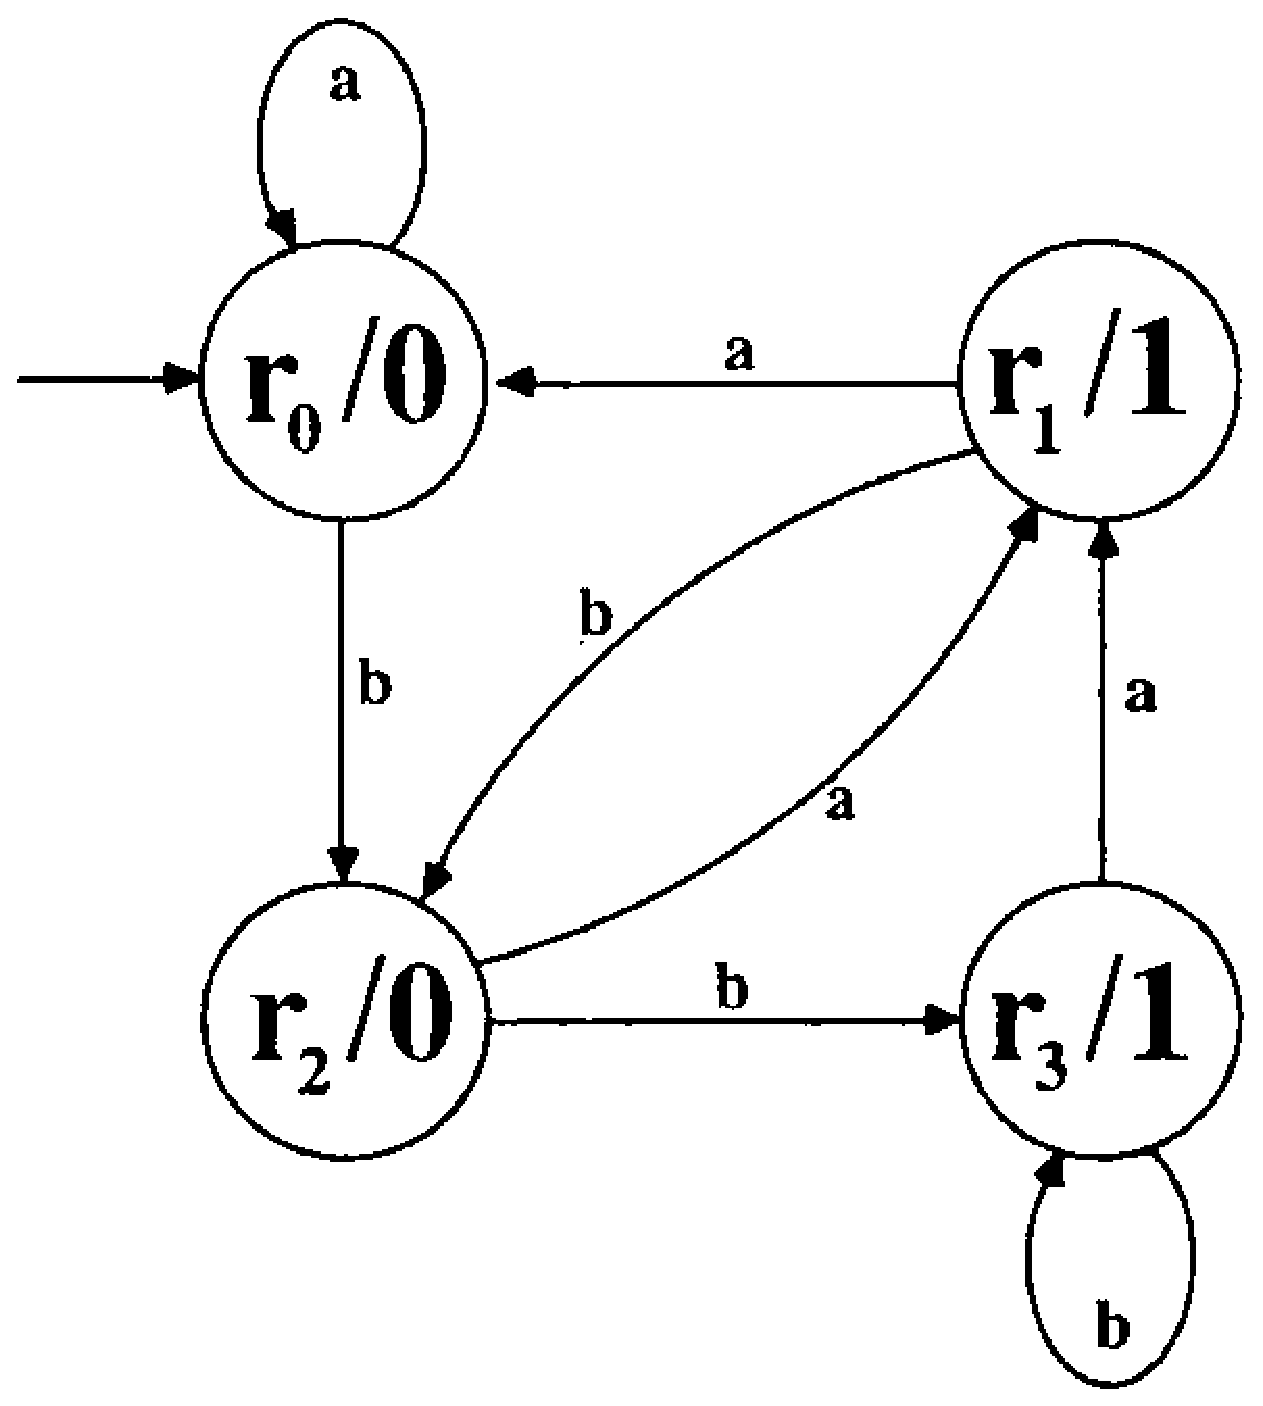
\epsfig{figure=ToFAfigures/fig7-6.eps,width=2.5in}}
\caption{The state transition diagram for the transducer discussed in Example
7.10}\label{fig-7.6}
\end{figure}

Results that were targeted toward a FST in the previous sections were specific
to Mealy machines. When the descriptor ``transducer'' appears in the theorems
and definitions presented earlier, the concept or result applies unchanged to
both FSTs and MSMs. Most of these results are alluded to but not restated in
this section. For example, \DBAR\ \index{extended state transition function \DBAR\! for MSM}
is defined like and behaves like the extended
state transition functions for DFAs and FSTs. On the other hand, because of the
drastic change in the domain of $\omega$, \OBAR\ must be modified as outlined
below in order for $\OBAR(s,x)$ to represent the output string produced when
starting at $s$ and processing $x$.

% Definition 7.17
\begin{dfn}\label{dfn-7.17}\index{extended output function \OBAR\! for MSM}
Given a MSM $A=\langle\Sigma,\Gamma,S,s_0,\delta,\omega\rangle$, the
\emph{\Index{extended output function}} for $A$, denoted again by \OBAR, is a
function $\omega$$: S \times \Sigma \rightarrow \Gamma^*$ defined recursively by:
\begin{enumerate}[i. ]
% handspaced vs. hardcoding i., ii.
\item $(\forall t \in S)\qquad\qquad\qquad\qquad\ \ \ \thinspace\thinspace\OBAR
	(t,\lambda)=\lambda$
\item $(\forall t \in S)(\forall x \in \Sigma^*)(\forall a \in \Sigma)
	(\OBAR(t,\pmb{a}x)=\omega(\delta(t,\pmb{a}))\cdot\OBAR
	(\delta(t,\pmb{a}),x)$
\end{enumerate}
\end{dfn}

Note that the domain of the function w has been extended further than usual:
in all previous cases, the domain was enlarged from $S \times \Sigma$ to
$S \times \Sigma^*$; in this instance, we are beginning with a domain of only
$S$ and still extending it to $S \times \Sigma^*$. The above definition allows
the following analog of Theorem \ref{thm-7.1} to remain essentially unchanged.

% Theorem 7.6
\begin{thm}\label{thm-7.6}
Let $\Sigma$ be an alphabet and $A=\langle\Sigma,\Gamma,S,s_0,\delta,\omega
\rangle$ be a Moore sequential machine. Then
\[ (\forall x \in \Sigma^*)(\forall y \in \Sigma^*)(\forall t \in S)(\OBAR(t,yx)
	=\OBAR(t,y) \cdot \OBAR(\DBAR(t,y),x)) \]
\emph{Proof.} The proof is by induction on $|y|$ (see the exercises and compare
with Theorem \ref{thm-1.1}).
\end{thm}

As before, the essence of a Moore machine is captured in the translation
function that the machine describes.

% Definition 7.18
\begin{dfn}\label{dfn-7.18}{\index{translation function!MSM}}
Given a MSM $M=\langle\Sigma,\Gamma,S,s_0,\delta,\omega\rangle$, the
\emph{translation function} for $M$, denoted by $f_M$, is the function
$f_M$$: \Sigma^* \rightarrow \Gamma^*$ defined by $f_M(x)=\OBAR(s_0,x)$.
\end{dfn}

Definition \ref{dfn-7.5} applies to Moore machines; two MSMs are equivalent if they
define the same translation. Indeed, it is possible for a Mealy machine to be
equivalent to a Moore machine, as shown by the transducers in Figures
\ref{fig-7.2} and \ref{fig-7.6}.

It is easy to turn a Moore machine $A=\langle\Sigma,\Gamma,S,s_0,\delta,\omega
\rangle$ into an equivalent Mealy machine $M=\langle\Sigma,\Gamma,S,s_0,\delta,
\omega'\rangle$. The first five parts of the transducer are unchanged. Only the
sixth component (the output function) must be redefined, as outlined below.

% Definition 7.19
\begin{dfn}\label{dfn-7.19}
Given a Moore machine $A=\langle\Sigma,\Gamma,S,s_0,\delta,\omega\rangle$, the
corresponding Mealy machine $M$ is given by $M=\langle\Sigma,\Gamma,S,s_0,
\delta,\omega'\rangle$, where $\omega'$ is defined by
\[ (\forall a \in \Sigma)(\forall s \in S)(\omega'(s,\pmb{a})=
	\omega(\delta(s,\pmb{a}))) \]
\end{dfn}

Pictorially, all arrows that lead \underline{into} a given state in the Moore machine should
be labeled in the corresponding Mealy machine with the output symbol for that
particular state. It follows easily from the definition that the corresponding
machines perform the same translation.

% Theorem 7.7
\begin{thm}\label{thm-7.7}\index{equivalent!transducers}
Given a Moore machine $A=\langle\Sigma,\Gamma,S,s_0,\delta,\omega\rangle$, the
corresponding Mealy machine\linebreak$M=\langle\Sigma,\gamma,S,s_0,\delta,\omega'\rangle$
is equivalent to $A$; that is, $(\forall x \in \Sigma^*)(f_M(x)=f_A(x))$.

\emph{Proof.} The proof is by induction on $|x|$ (see the exercises).
\end{thm}

\subsection*{Example 7.11}

Let $A=\langle\Sigma,\Gamma,S,r_0,\delta,\omega\rangle$ be the Moore machine
given in Figure \ref{fig-7.6}. The corresponding Mealy machine $M=\langle\Sigma,\Gamma,S,
s_0,\delta,\omega'\rangle$ is then given by
\[ \Sigma=\{\pmb{a},\pmb{b}\},\quad \Gamma=\{\pmb{0},\pmb{1}\},\quad
	S=\{r_0,r_1,r_2,r_3\},\quad s_0 = r_0 \]
and the state transition table and the output function table are specified as
in Tables 7.4a and 7.4b.
% Table 7.3a & 7.3b
\begin{table}[h]\label{table-7.3}
\begin{center}
\begin{tabular}{c|cc}
\multicolumn{3}{c}{Table 7.3a} \\
$\delta$ & $\pmb{a}$ & $\pmb{b}$ \\
\hline
$r_0$ & $r_0$ & $r_2$ \\
$r_1$ & $r_0$ & $r_2$ \\
$r_2$ & $r_1$ & $r_3$ \\
$r_3$ & $r_1$ & $r_3$
\end{tabular}
$\qquad$
\begin{tabular}{c|cc}
\multicolumn{3}{c}{Table 7.3b} \\
$\omega'$ & $\pmb{a}$ & $\pmb{b}$ \\
\hline
$r_0$ & $\pmb{0}$ & $\pmb{0}$ \\
$r_1$ & $\pmb{0}$ & $\pmb{0}$ \\
$r_2$ & $\pmb{1}$ & $\pmb{1}$ \\
$r_3$ & $\pmb{1}$ & $\pmb{1}$
\end{tabular}
\end{center}
\end{table}
The new Mealy machine is shown in Figure \ref{fig-7.7}. Note that the arrow labeled
$\pmb{a}$ leaving $r_1$ now has a $\pmb{0}$ associated with it, since the state at
which the arrow pointed $(r_0/\pmb{0})$ originally output a $\pmb{0}$.

% Figure 7.7
\begin{figure}
\centerline{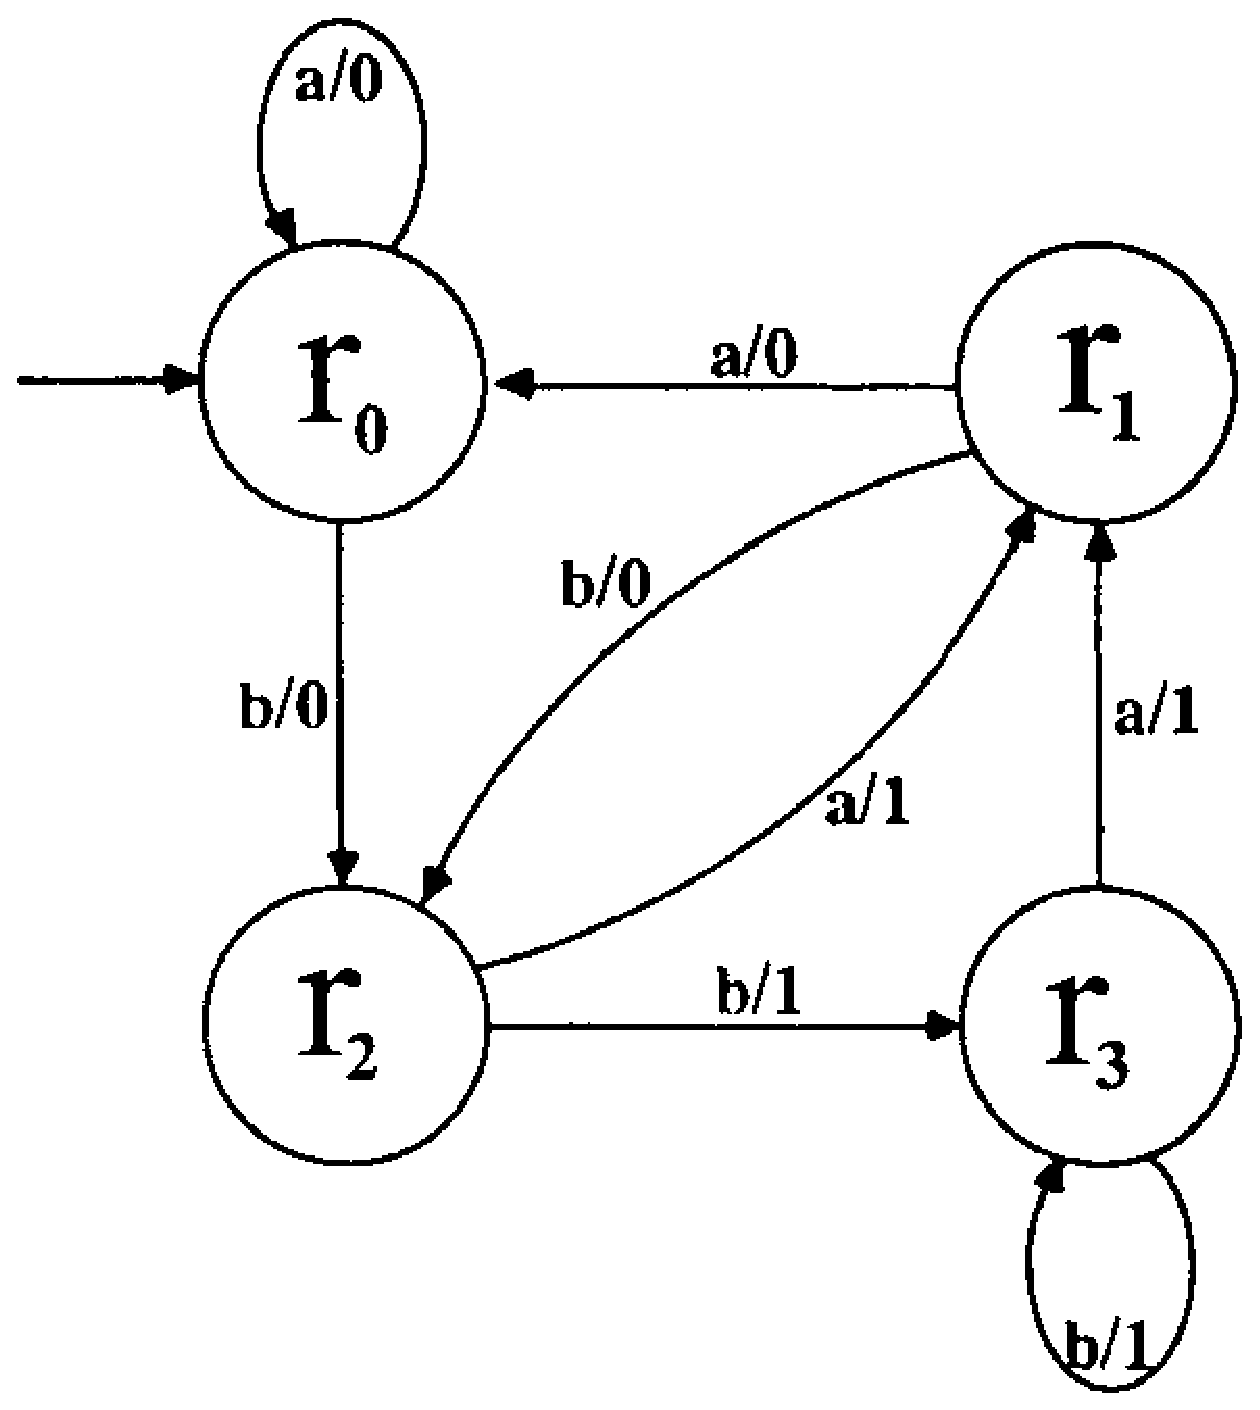
\epsfig{figure=ToFAfigures/fig7-7.eps,width=2.5in}}
\caption{The state transition diagram for the Mealy machine $M$ in Example 7.11}\label{fig-7.7}
\end{figure}

In a similar fashion, an equivalent Moore machine can be defined that
corresponds to a given Mealy machine. However, due to the more restricted nature
of the output function of the Moore constructs, the new machine will generally
need more states to perform the same translation.

The idea behind the construct is to break each state in the Mealy machine up
into a group of several similar states in the Moore machine, each of which
prints a different output symbol. The new transition function mimics the old
one; if state $r$ maps to state $t$ in the Moore machine, then any state in the
group corresponding to $r$ will map to one particular state in the group of
states corresponding to $t$. The particular state within the group is chosen in
a manner that will guarantee that the appropriate output symbol will be printed.
This construct is implemented in the following definition.

% Definition 7.20
\begin{dfn}\label{dfn-7.20}
Given a Mealy machine $M=\langle\Sigma,\Gamma,S,s_0,\delta,\omega\rangle$, the
corresponding Moore machine $A$ is given by $A=\langle\Sigma,\Gamma,S \times
\Gamma,\langle s_0,\alpha\rangle,\delta',\omega'\rangle$, where $\alpha$ is
an (arbitrary) member of\, $\Gamma$,
\[ \delta'\text{ is defined by }(\forall s \in S)(\forall\pmb{b}\in\Gamma)
	(\forall\pmb{a}\in\Sigma)(\delta'(\langle s,\pmb{b}\rangle, \pmb{a})
        =\langle\delta(s,\pmb{a}),\omega(s,\pmb{a})\rangle) \]
and
\[ \omega'\text{ is defined by }(\forall s \in S)(\forall\pmb{b}\in\Gamma)
	(\omega'(\langle s,\pmb{b}\rangle) = \pmb{b}). \]
\end{dfn}

% Theorem 7.8
\begin{thm}\label{thm-7.8}\index{equivalent!transducers}
Given a Mealy machine $M=\langle\Sigma,\Gamma,S,s_0,\delta,\omega\rangle$, the
corresponding Moore machine $A=\langle\Sigma,\Gamma,S,s_0,\delta',\omega'\rangle$
is equivalent to $M$; that is, $(\forall x \in \Sigma^*)(f_A(x)=f_M(x))$,

\emph{Proof.} The proof is by induction on $|x|$ (see the exercises).
\end{thm}

Since every Mealy machine has an equivalent Moore machine and every Moore
machine has an equivalent Mealy machine, either construct can be used as a
basis of what was meant by a translation $f$ being finite transducer definable.

% Corollary 7.8
\begin{cor}\label{cor-7.8}
A translation $J$ is FTD iff $f$ can be defined by a FST $M$ iff $f$ can be
defined by a MSM $A$.

\emph{Proof.} The proof is immediate from the definition of FTD and Theorems
\ref{thm-7.7} and \ref{thm-7.8}.
\end{cor}

\subsection*{Example 7.12}

Consider the Mealy machine $B$ from Figure \ref{fig-7.3}. The corresponding Moore machine
$A=\langle\Sigma,\Gamma,S,q_0,\delta,\omega\rangle$ is given by
\begin{center}\begin{tabular}{l}
$\Sigma=\{\pmb{a},\pmb{b}\}$ \\
$\Gamma=\{\pmb{0},\pmb{1}\}$ \\
$S=\{\langle s_0,\pmb{0}\rangle,\langle s_0,\pmb{1}\rangle,\langle s_1,\pmb{0}
	\rangle,\langle s_1,\pmb{1}\rangle\}$ \\
$q_0 = \langle s_0,\pmb{1}\rangle$ \\
$\omega(\langle s_0,\pmb{0}\rangle)=\pmb{0},\quad\omega(\langle s_0,\pmb{1}
	\rangle)=\pmb{1},\quad\omega(\langle s_1,\pmb{0}\rangle)=\pmb{0},\quad
	\omega(\langle s_1,\pmb{1}\rangle)=\pmb{1}$
\end{tabular}\end{center}
and the state transition table is specified as in Table 7.4.
% Table 7.4
\begin{table}[h]\label{tbl-7.4}
\begin{center}\begin{tabular}{c|cc}
\multicolumn{3}{c}{Table 7.4} \\
$\delta$ & $\pmb{a}$ & $\pmb{b}$ \\
\hline
$\langle s_0,\pmb{0}\rangle$ & $\langle s_0,\pmb{0}\rangle$ & $\langle s_1,
	\pmb{0}\rangle$ \\
$\langle s_0,\pmb{1}\rangle$ & $\langle s_0,\pmb{0}\rangle$ & $\langle s_1,
	\pmb{0}\rangle$ \\
$\langle s_1,\pmb{0}\rangle$ & $\langle s_0,\pmb{1}\rangle$ & $\langle s_1,
	\pmb{1}\rangle$ \\
$\langle s_1,\pmb{1}\rangle$ & $\langle s_0,\pmb{1}\rangle$ & $\langle s_1,
	\pmb{1}\rangle$
\end{tabular}\end{center}
\end{table}

% Figure 7.8
\begin{figure}
\centerline{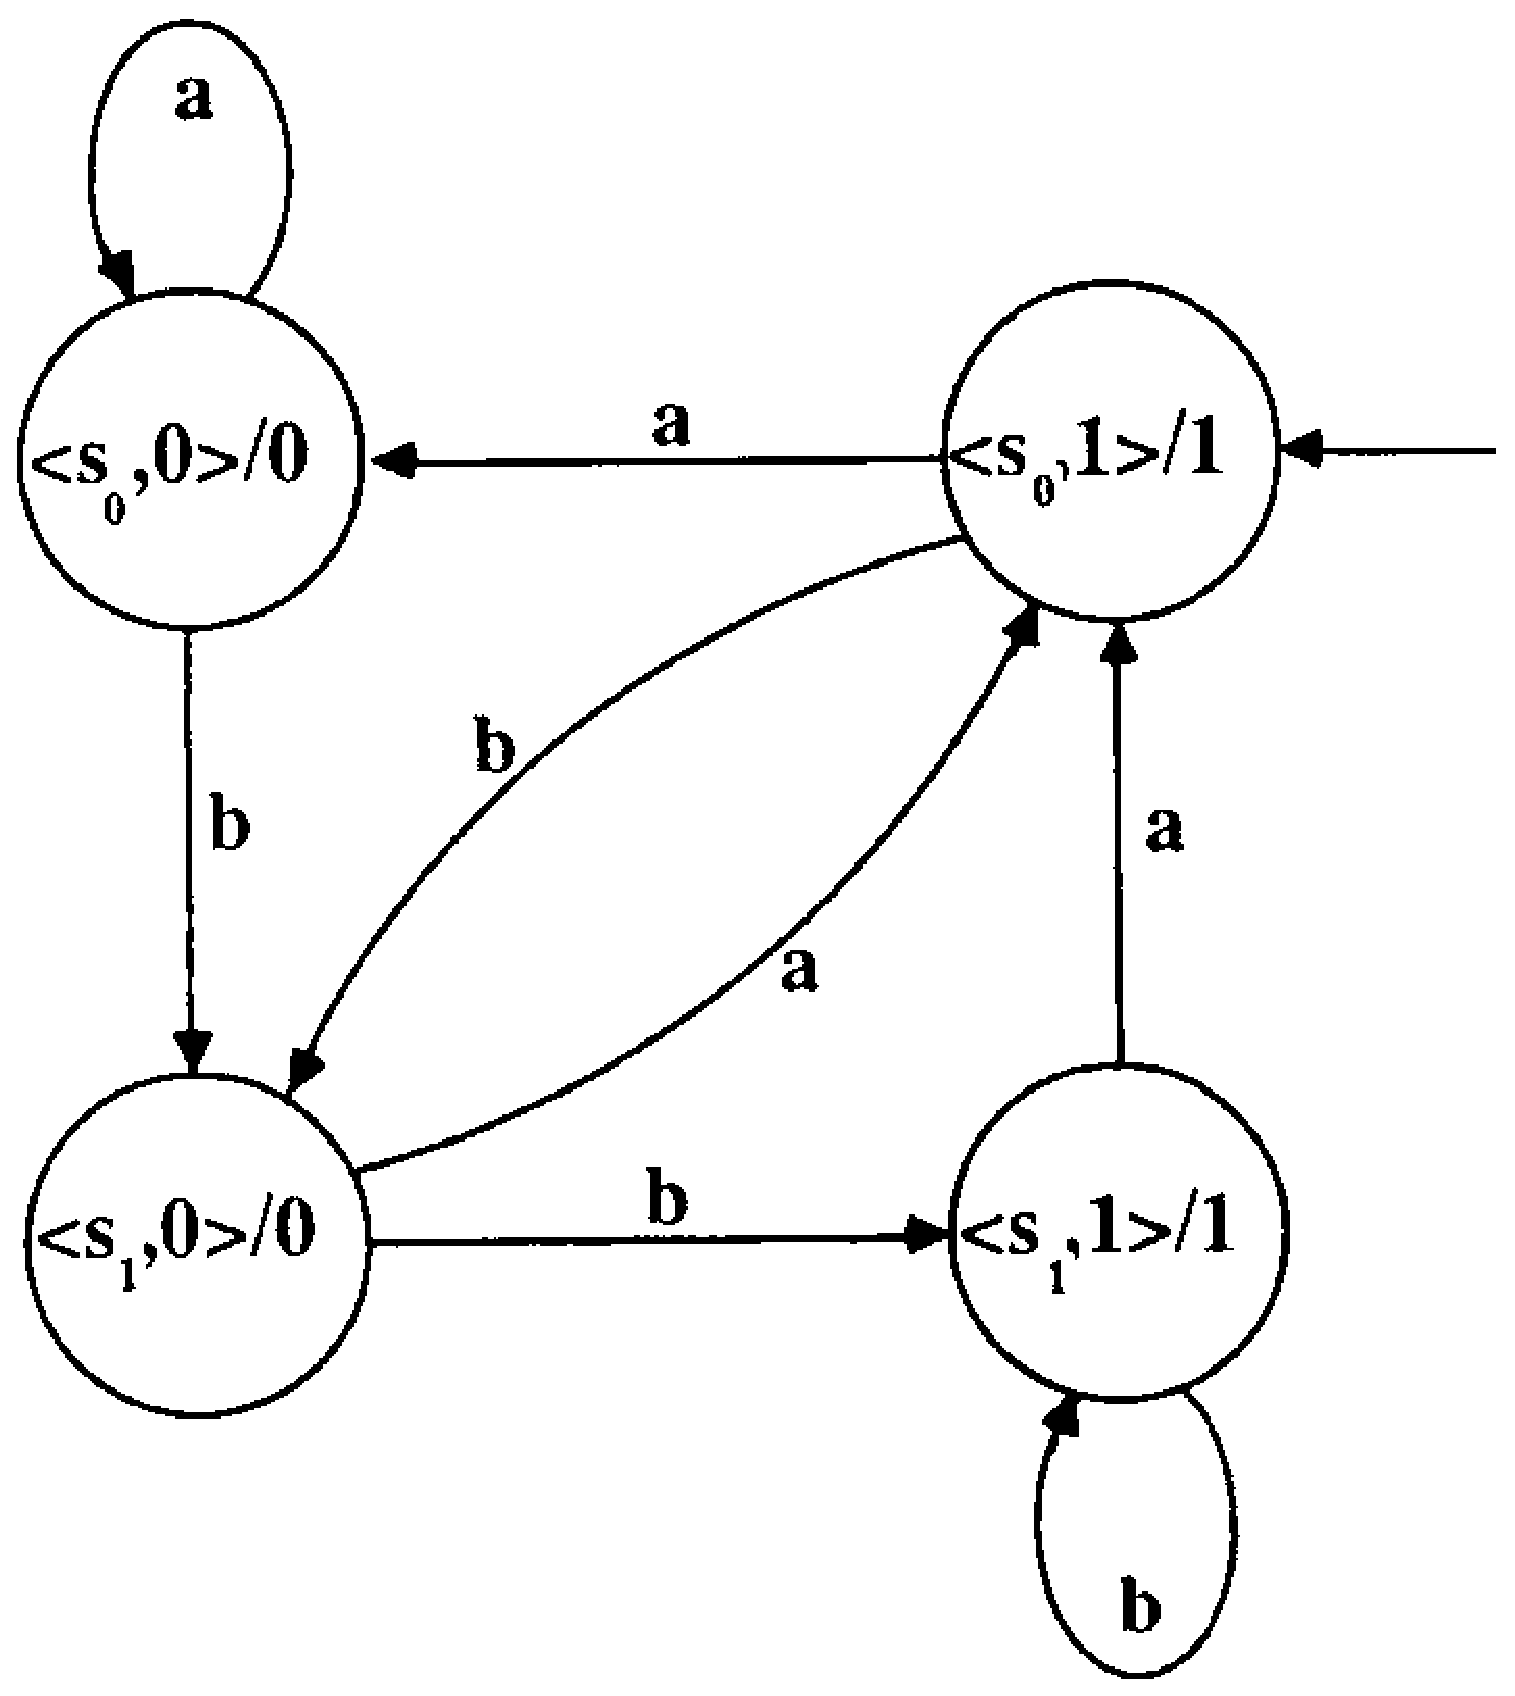
\epsfig{figure=ToFAfigures/fig7-8.eps,width=2.5in}}
\caption{The state transition diagram for the Moore machine A in Example
7.12}\label{fig-7.8}
\end{figure}

Figure \ref{fig-7.8} displays this new Moore machine. Note that this transducer $A$,
except for the placement of the start state, looks very much like the Moore
machine
$C$ given in Figure \ref{fig-7.6}. Indeed, any ordered pair that is labeled with the
original start state would be an acceptable choice for the new start state in
the corresponding Moore machine. For example, the automaton $A'$, which is
similar to $A$ but utilizes $\langle s_0,\pmb{0}\rangle$ as the new start state, is another
Moore machine that is equivalent to the original Mealy machine $B$. The
transition diagram for $A'$ is shown in Figure \ref{fig-7.9}. In fact, by appropriately
recasting the definition of isomorphism so that it applies to Moore sequential
machines, it can be shown that $A'$ and $C$ are isomorphic. The definition of
isomorphic again guarantees that a renaming of the states can be found that
preserves start states, transition functions, and output functions. Indeed, the
definition of isomorphism agrees with that of Mealy machines (and of DFAs, for
that matter) except in the specification of the correspondence between output
functions. The formal definition is given below.

% Figure 7.9
\begin{figure}
\centerline{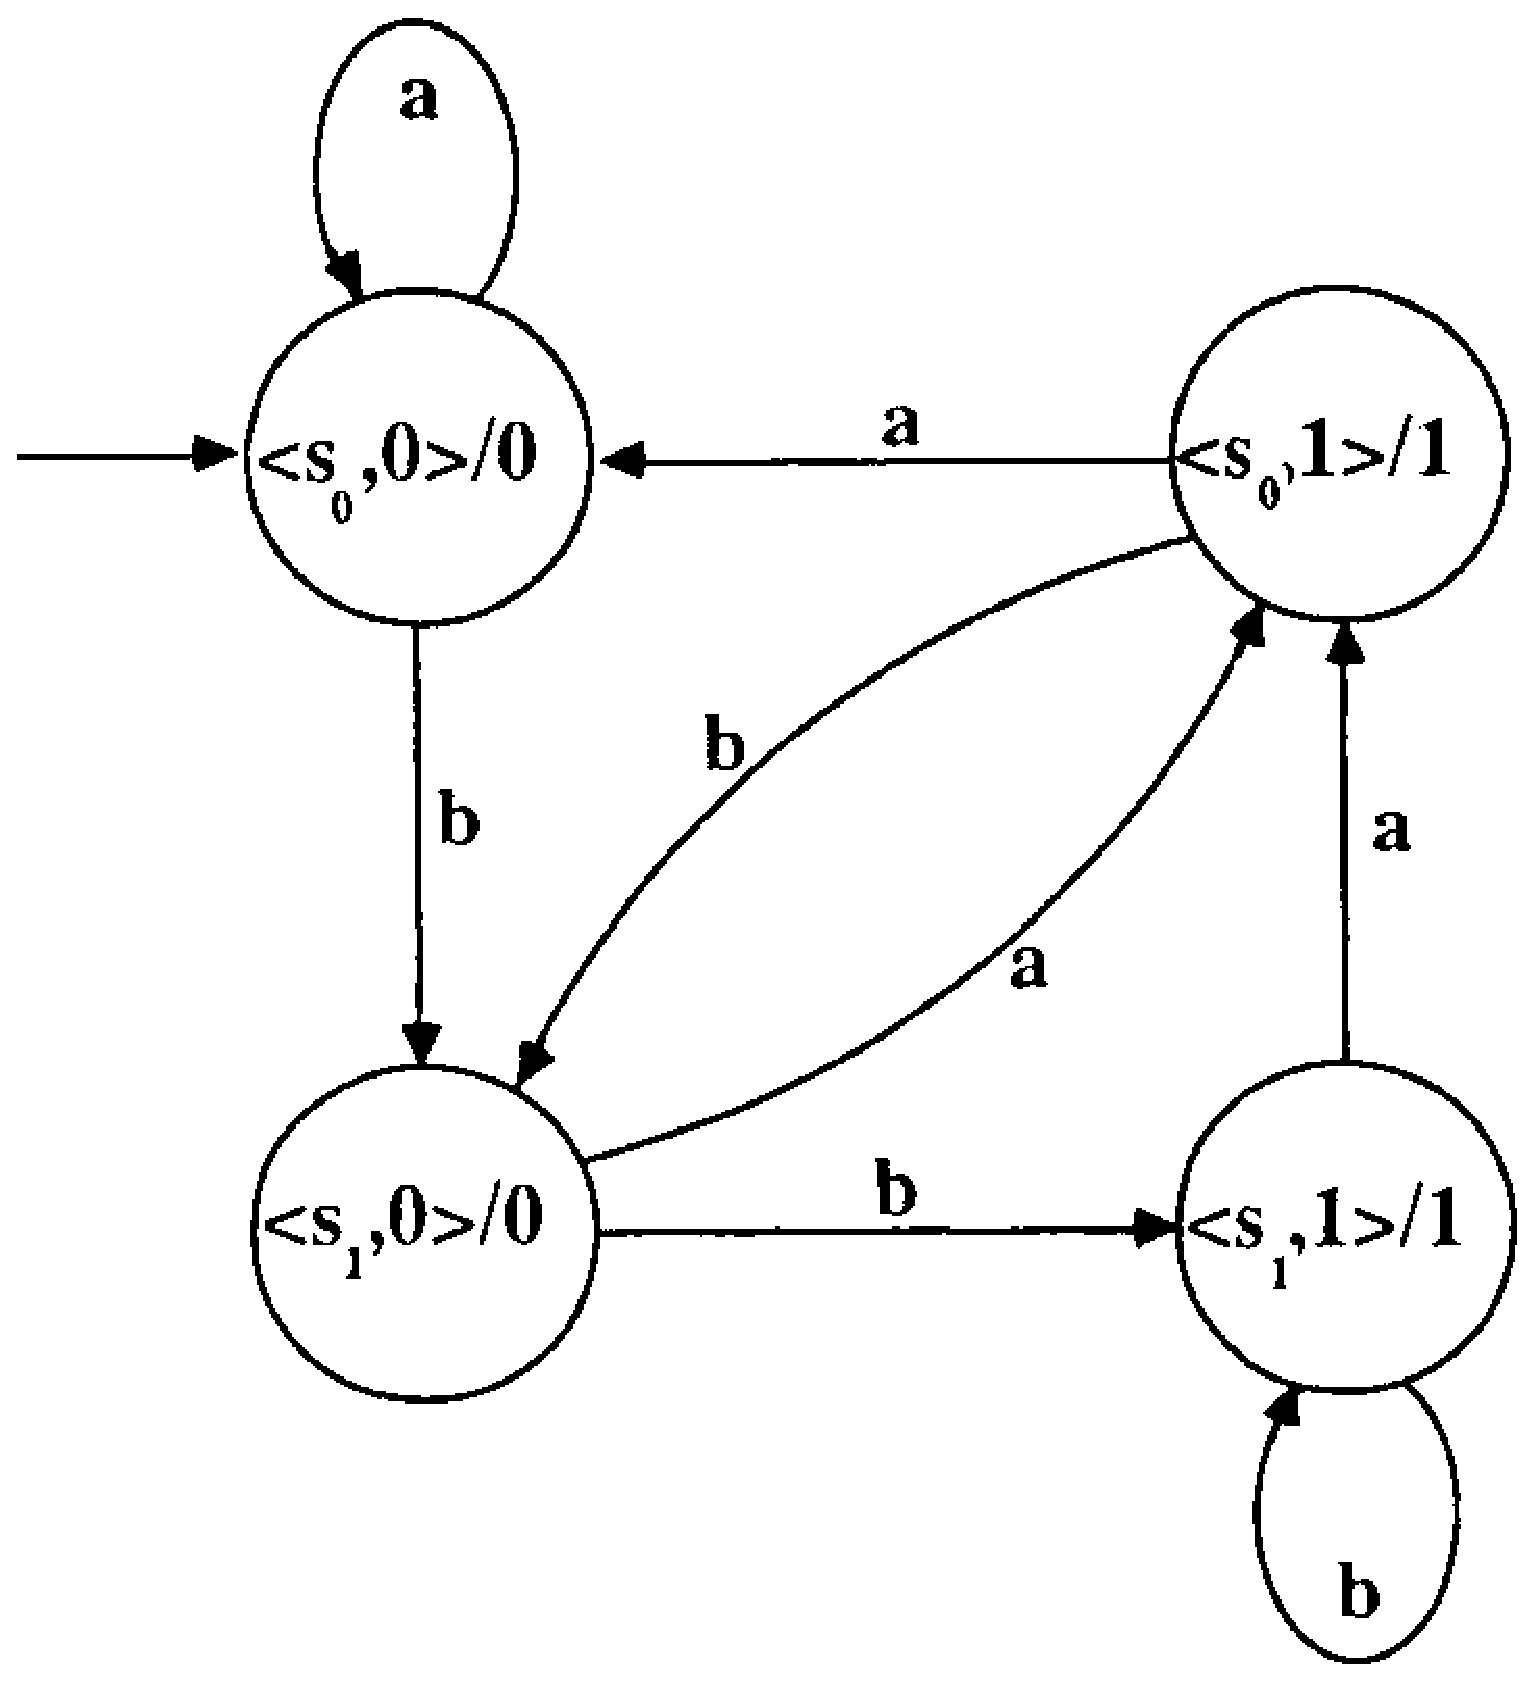
\epsfig{figure=ToFAfigures/fig7-9.eps,width=2.5in}}
\caption{The state transition diagram for the Moore machine $A'$ in Example
7.12}\label{fig-7.9}
\end{figure}

% Definition 7.21
\begin{dfn}\label{dfn-7.21}
Given two MSMs
\[ A=\langle\Sigma,\Gamma,S_A,s_{0_A},\delta_A,\omega_A\rangle\quad\text{ and }
	B=\langle\Sigma,\Gamma,S_B,s_{0_B},\delta_B,\omega_A\rangle, \]
and a function $\mu$$: S_A \rightarrow S_B,\ \mu$ is called a \emph{\Index{Moore
machine isomorphism}} from $A$ to $B$ iff the following five conditions hold:\emph{isomorphism}\index{isomorphism!between MSMs}
\begin{enumerate}[i.]
\item $\mu(s_{0_A}) = s_{0_B}$.
\item $(\forall s \in S_A)(\forall\pmb{a}\in\Sigma)(\mu(\delta_A(s,\pmb{a})) =
	\delta_B(\mu(s),\pmb{a}))$.
\item $(\forall s \in S_A)(\omega_A(s) = \omega_B(\mu(s)))$.
\item $\mu$ is a one-to-one function between $S_A$ and $S_B$.
\item $\mu$ is onto $S_B$.
\end{enumerate}
\end{dfn}

\subsection*{Example 7.13}

The two Moore machines $A'$ in Figure \ref{fig-7.9} and $C$ in Figure \ref{fig-7.6} are indeed
\Index{isomorphic}. There is a function $\mu$ from the states of $A'$ to the states of
$C$ that satisfies all five properties of an isomorphism. This correspondence is
given by $\mu(\langle s_0,\pmb{0}\rangle) = r_0,\ \mu(\langle s_0,\pmb{1}\rangle)
=r_1,\ \mu(\langle s_1,\pmb{0}\rangle)=r_2$, and $\mu(\langle s_1,\pmb{1}\rangle)=r_3$,
succinctly defined by $\mu(\langle s_i,j\rangle)=r_{2i+j}$, for $i,j \in
\{\pmb{0},\pmb{1}\}$. As before, a homomorphism is meant to represent a
correspondence between states that preserves the algebraic structure of the
transducer without necessarily being a bijection.

% Definition 7.22
\begin{dfn}\label{dfn-7.22}
Given two MSMs
\[ A=\langle\Sigma,\Gamma,S_A,s_{0_A},\delta_A,\omega_A\rangle\quad\text{ and }
	B=\langle\Sigma,\Gamma,S_B,s_{0_B},\delta_B,\omega_A\rangle, \]
and a function $\mu$$: S_A \rightarrow S_B,\ \mu$ is called a \emph{\Index{Moore
machine homomorphism}} from $A$ to $B$ iff the following three conditions hold:
\index{homomorphism!between MSMs}

\begin{enumerate}[i.]
\item $\mu(s_{0_A}) = s_{0_B}$.
\item $(\forall s \in S_A)(\forall\pmb{a}\in\Sigma)(\mu(\delta_A(s,\pmb{a})) =
	\delta_B(\mu(s),\pmb{a}))$.
\item $(\forall s \in S_A)(\omega_A(s) = \omega_B(\mu(s)))$.
\end{enumerate}
\end{dfn}

The isomorphism $\mu$ discussed in Example 7.13 is also a homomorphism.
Preserving the algebraic structure of the transducer guarantees that the
translation is also preserved: if $A$ and $B$ are homomorphic, then they are
equivalent. The homomorphism criterion that applies to single letters once again
extends to similar statements about strings, as outlined in Lemma \ref{lmm-7.5}.

% Lemma 7.5
\begin{lmm}\label{lmm-7.5}
If $\mu$$: S_A \rightarrow S_B$ is a homomorphism between two MSMs
\[ A=\langle\Sigma,\Gamma,S_A,s_{0_A},\delta_A,\omega_A\rangle\quad\text{ and }
	B=\langle\Sigma,\Gamma,S_B,s_{0_B},\delta_B,\omega_A\rangle, \]
then
\[ (\forall s \in S_A)(\forall x \in \Sigma^*)(\mu(\DBAR_A(s,x))=\DBAR_B
	(\mu(s),x)) \]
and
\[ (\forall s \in S_A)(\forall x \in \Sigma^*)(\OBAR_A(s,x)=\OBAR_B
	(\mu(s),x)). \]
\emph{Proof.} The proof is by induction on $|x|$ (see the exercises).
\end{lmm}

% Corollary 7.9
\begin{cor}\label{cor-7.9}
If $\mu$$:S_A \rightarrow S_B$ is a homomorphism between two MSMs
$A=\langle\Sigma,\Gamma,S_A,s_{0_A},\delta_A,\omega_A\rangle$ and
$B=\langle\Sigma,\Gamma,S_B,s_{0_B},\delta_B,\omega_B\rangle$, then $A$ is
equivalent to $B$; that is, $f_A = f_B$.

\emph{Proof.} The proof follows immediately from Lemma \ref{lmm-7.5} and the definition
of $f_M$.
\end{cor}

It is interesting to note that the MSMs $A$ in Figure \ref{fig-7.8} and $A'$ in Figure
\ref{fig-7.9} are not isomorphic. In fact, there does not even exist a homomorphism (in
either direction) between $A$ and $A'$ since the start states print different
symbols, and rules (i) and (iii) therefore conflict. The absence of an
isomorphism in this instance illustrates that an analog to Theorem \ref{thm-7.5} cannot be
asserted under the definition of Moore sequential machines presented here.
Observe that $A$ and $A'$ are equivalent and they are both minimal (four states
are necessary in a Moore machine to perform this translation), yet they are not
isomorphic. The reader should contrast this failure with the analogous statement
about Mealy machines in Theorem \ref{thm-7.5}.

Producing a result comparable to Theorem \ref{thm-7.5} is not possible without a
fundamental adjustment of at least one of the definitions. One possibility is to
drop the distinguished start state from the definition of the Moore machine.
This removes condition (i) from the isomorphism definition and thereby resolves
the conflict between (i) and (iii). We have already noted that many applications
do not require a distinguished start state (such as elevators and traffic signal
controls), which makes this adjustment not altogether unreasonable.

A more common alternative is to decree that a Moore sequential machine first
print the character specified by the start state upon being turned on (before
any of the input tape is read) and then proceed as before. This results in
output strings that are always one symbol longer than the corresponding input
strings, and the length-preserving property of transducers is thereby lost. A
more substantial drawback results from the less natural correspondence between
Mealy and Moore machines: no FST can be truly equivalent to any MSM since
translations would not even be of the same length.

The advantage of this decree is that machines like $A$ and $A'$ (from Figures
\ref{fig-7.8} and \ref{fig-7.9}) would no longer be equivalent, and hence they would not be expected
to be isomorphic. Note that equivalence is lost since, under the new decree for
translations, they would produce different output when presented with, say,
$\lambda$ as input: $A$ would print $\pmb{1}$ while $A'$ would produce
$\pmb{0}$. Our definition of a MSM (Definition \ref{dfn-7.16}) was chosen to remain
compatible with the translations obtained from Mealy machines and to preserve a
distinguished state as the start state; these advantages were obtained at the
expense of a convenient analog to Theorem \ref{thm-7.5}.

A third, and perhaps the best, alternative is to modify what we mean by a MSM
isomorphism. Definition \ref{dfn-7.21} can be rephrased to relax the condition that the
start states of the two machines must print the same character.

As with Mealy machines, Moore machines can also be minimized, and a reduced and
connected MSM is guaranteed to be the smallest MSM which performs that
translation. Note that Definitions \ref{dfn-7.4} (FTD), \ref{dfn-7.5} (equivalence), \ref{dfn-7.9}
(isomorphic), \ref{dfn-7.10} (connected), \ref{dfn-7.12} (state equivalence relation), \ref{dfn-7.13}
(reduced), and \ref{dfn-7.15}\index{equivalent!MSM states} ($i^{\text th}$ relation) have been phrased to encompass both forms
of transducers. Minor changes (generally involving the domain of the output
function) are all that is necessary to make the remaining definitions and
results conform to the Moore constructs. We begin with a formal definition of
minimality, which is in essence the same as the definitions presented for DFAs
and FSTs (Definitions \ref{dfn-2.7} and \ref{dfn-7.6}).

% Definition 7.23
\begin{dfn}\label{dfn-7.23}
Given a MSM $A=\langle\Sigma,\Gamma,S_A,s_{0_A},\delta_A,\omega_A\rangle,\ A$ is
the \emph{\Index{minimal Moore machine} for the translation} $f_A$ iff for all MSMs
$B=\langle\Sigma,\Gamma,S_B,s_{0_B},\delta_B,\omega_B\rangle$ for which
$f_A = f_B,\ \|S_A\| \leq \|S_B\|$.
\end{dfn}

A connected Moore machine is essential to minimality. The previous definition
of connectedness (Definition \ref{dfn-7.10}) suffices for both FSTs and MSMs and was
therefore phrased to apply to all transducers, rather than to one specific
type of transducer. For an arbitrary Moore machine, the algorithm for finding
the set of accessible states is unchanged; transitions are followed from the
start state until no further new states are found. The connected version of a
MSM is again obtained by paring down the state set to encompass only the
connected states and restricting the $\delta$ and $\omega$ functions to the
smaller domain.

% Definition 7.24
\begin{dfn}\label{dfn-7.24}\index{M connected (MSM $M^c$)}\index{A@$A^c$ (A connected)!for MSM}
Given a MSM $M=\langle\Sigma,\Gamma,S,s_0,\delta,\omega\rangle$, define the
transducer $M^c =\langle\Sigma,\Gamma,S^c,s^c_0,\delta^c,\omega^c\rangle$,
called \emph{M connected}, by
\begin{center}\begin{tabular}{l}
$S^c=\{s \in S^c$ $|$ $\exists x \in \Sigma^* \ni \DBAR(s_0,x) = s\}$ \\
$s^c_0 = s_0$
\end{tabular}\end{center}
$\delta^c$ is essentially the restriction of $\delta$ to $S^c \times \Sigma:\ 
(\forall\pmb{a}\in\Sigma)(\forall s \in S^c)(\delta^c(s,\pmb{a}) = 
\delta(s,\pmb{a}))$, and $\omega^c$ is the restriction of $\omega$ to
$S^c \times \Sigma:\ (\forall s \in S^c)(\omega^c(s) = \omega(s))$.
\end{dfn}

The concept of a reduced Moore machine and the definition of the state
equivalence relation are identical in spirit and in form to those presented
for Mealy machines (Definitions \ref{dfn-7.12} and \ref{dfn-7.13}). The definition that outlines
how to reduce a Moore machine by coalescing states differs from that given for
FSTs (Definition \ref{dfn-7.14}) only in the specification of the output function. In
both Definition \ref{dfn-7.14} and the following Moore machine analog, the value $\omega$
takes for an equivalence class is determined by the value given for a
representative of that equivalence class. As before, this natural definition for
the output function can be shown to be well defined (see the exercises).

% Definition 7.25
\begin{dfn}\label{dfn-7.25}\index{A @$ A/_{E_A}$ (A modulo $E_A$)!for MSM}
Given a MSM $M=\langle\Sigma,\Gamma,S,s_0,\delta,\omega\rangle$, define
\Index{M$/\!\!_{E_M}$}, \emph{$M$ modulo its state equivalence relation}, by
$M/\!\!_{E_M}=\langle\Sigma,\Gamma,S_{E_M},s_{0_{E_M}},\delta_{E_M},\omega_{E_M}
\rangle$, where
\begin{center}\begin{tabular}{l}
$S_{E_M}=\{[s]_{E_M}$ $|$ $ s \in S\}$ \\
$s_{0_{E_M}} = [s_0]_{E_M}$
\end{tabular}\end{center}
$\delta_{E_M}$ is defined by
\[ (\forall\pmb{a}\in\Sigma)(\forall [s] \in S_{E_M})(\delta_{E_M}
	([s]_{E_M},\pmb{a})=[\delta(s,\pmb{a})]_{E_M}), \]
and $\omega_{E_M}$ is defined by
\[ (\forall [s] \in S_{E_M})(\omega_{E_M}([s]_{E_M}) = \omega(s)) \]
\end{dfn}

The Moore machine $M/\!\!_{E_M}$ has all the properties attributed to the Mealy
version. Without changing the nature of the translation, it is guaranteed to
produce a MSM which is reduced.

% Theorem 7.9
\begin{thm}\label{thm-7.9}
Given a MSM $M=\langle\Sigma,\Gamma,S,s_0,\delta,\omega\rangle$:
\begin{enumerate}[a.]
\item $M/\!\!_{E_M}=\langle\Sigma,\Gamma,S_{E_M},s_{0_{E_M}},\delta_{E_M},
	\omega_{E_M}\rangle$ is equivalent to $M$.
\item $M/\!\!_{E_M}$ is reduced.
\item If $M$ is connected, so is $M/\!\!_{E_M}$.
\item Given a FTD function $f$, the minimal Moore machine corresponding to $f$
must be reduced.
\end{enumerate}

\emph{Proof.} The proof is similar to Theorem \ref{thm-7.4} (see the exercises).
\end{thm}

As mentioned earlier, the definition of a MSM chosen here denies a convenient
analog to Theorem \ref{thm-7.5}. However, a reduced and connected Moore machine must be
minimal.

% Theorem 7.10
\begin{thm}\label{thm-7.10}
\item Given a MSM $M$:
\begin{enumerate}[(a)]
\item
A necessary and sufficient condition for $M$ to be
	minimal is that $M$ is both reduced and connected.
\item $M^c\!/\!\!_{E_{M^c}}$, is minimal.
\end{enumerate}

\emph{Proof.} See the exercises.
\end{thm}

The minimal Moore machine corresponding to a MSM $M$ can thus be obtained
if the connected state set and the state equivalence relation can be computed.
The algorithm for calculating the accessible states is the same as before, and
computing the state equivalence relation will again be accomplished using the
concept of the $i$th state equivalence relation (Definition \ref{dfn-7.15}). All the
results proved previously in Lemma \ref{lmm-7.3} still hold, showing that successive
calculations are guaranteed to halt and produce $E_M$. All that remains is to
specify both a starting point and a way to find the next relation from the
current $E_{iM}$.

With Mealy machines, $E_{0M}$ consisted of one single equivalence class, since
$\lambda$ could not distinguish between states. All states were therefore
related to each other under $E_{0M}$. With Moore machines, different states
cause different letters to be printed. $E_{0M}$ can therefore be thought of as
grouping together states that print the same symbol.

% Lemma 7.6
\begin{lmm}\label{lmm-7.6}
Given a MSM $M=\langle\Sigma,\Gamma,S,s_0,\delta,\omega\rangle$:
\begin{enumerate}[(a)]
\item $E_{0M}$ is defined by $s E_{0M} t \Leftrightarrow (\omega(s)=\omega(t))$.
\item For $i \geq 0$, $E_{i+1M}$ can be computed from $E_{iM}$ as follows:
\[ (\forall s \in S)(\forall t \in S)(\forall i \geq 0)(s E_{i+1M} t
	\Leftrightarrow s E_{iM} t \wedge (\forall\pmb{a}\in\Sigma)
	(\delta(s,\pmb{a})E_{iM}\delta(t,\pmb{a}))). \]
\end{enumerate}

\emph{Proof.} The proof is essentially the same as in Chapter \ref{ch-3} (see Theorem
\ref{thm-3.8}).
\end{lmm}

% Corollary 7.10
\begin{cor}\label{cor-7.10}
Given a MSM $M=\langle\Sigma,\Gamma,S,s_0,\delta,\omega\rangle$, there is an
\emph{algorithm} for computing $E_M$.

\emph{Proof.} See the exercises.
\end{cor}

$E_{0M}$ will generally have one equivalence class for each symbol in $\Gamma$;
$rk(E_{0M})$ could be less than $\|\Gamma\|$ if some output symbols are not
printed by any state (remember that equivalence classes are by definition
nonempty). The rule for computing $E_{i+1M}$ from $E_{iM}$ is identical to that
given for Mealy machines (and DFAs); only the starting point, $E_{0M}$, had to
be redefined for Moore machines (compare with Lemma \ref{lmm-7.4}). Lemmas \ref{lmm-7.3} and \ref{lmm-7.6}
imply that there is an algorithm for finding $E_M$ for any Moore machine $M$;
this was the final computation needed to produce $M^c\!/\!\!_{E_{M^c}}$, which will be
the minimal Moore machine equivalent to the MSM $M$.

% Corollary 7.11
\begin{cor}\label{cor-7.11}
Given a MSM $M=\langle\Sigma,\Gamma,S,s_0,\delta,\omega\rangle$, there is an
\emph{algorithm} for computing the minimal machine equivalent to M.

\emph{Proof.} See the exercises.
\end{cor}

\section{Transducer Applications and Circuit Implementation}\label{7.4}

The vending machine example that began this chapter showed that the transducer
was capable of modeling many of the machines we deal with in everyday life. This
section gives examples of several types of applications and then shows how to
form the circuitry that will implement such transducers. Transducers can be used
not only to model physical machinery, but can also form the basis for
computational algorithms. The following example can be best thought of not as a
model of a machine that receives files, but as a model of the behavior of the
computer algorithm that specifies how such files are to be received.

\subsection*{Example 7.14}

The transducer metaphor is often used to succinctly describe the structure of
many algorithms commonly used in computer applications, most notably in network
communications. \emph{Kermit}\index{Kermit protocol!FST implementation} is a popular means of transferring files
between mainframes and microcomputers. A transfer is accomplished by the send
portion of Kermit on the source host exchanging information with the receive
portion of Kermit on the destination host. The two processes communicate by
exchanging \emph{packets} of information; these packets comprise the input
alphabet of our model. When the Kermit protocol was examined in Chapter \ref{ch-1}
(Example 1.16), it was noted that a full description of the algorithm must also
describe the action taken upon receipt of an incoming packet; these actions
comprise the output alphabet of our model. During a file transfer, the states of
the receiving portion of Kermit on the destination host are $R$ (awaiting a
transfer request), $RF$ (awaiting the name of the file to be transferred),
$RD$ (awaiting more data to be placed in the new file), and $A$ (abort due to an
unrecoverable error). The set of states will again be $A,R,RD,RF\}$.

Expected inputs are represented by  $\pmb{S}$ (an initialization packet, indicating
that a transfer is requested), $\pmb{H}$ (a header packet, containing the name of
one of the files to be created and opened), $\pmb{D}$ (a data packet), $\pmb{Z}$ (an
end of file marker [\Index{EOF packet}], signaling that no more data need be placed in the currently
opened file), and $\pmb{B}$ (break, signaling the end of transmission). Unexpected
input, representing a garbled transmission, is denoted by $\pmb{X}$. The input
alphabet is therefore $\Sigma=\{\pmb{B},\pmb{D},\pmb{H},\pmb{S},\pmb{X},
\pmb{Z}\}$.

When Kermit receives a recognizable packet [that is also appropriate at the
current stage of the conversation], it sends an acknowledgment (ACK)
back to the other host. This action will be represented in the output alphabet
by the symbol $\pmb{Y}$. When the receiver expects and gets a valid header packet,
it opens the appropriate file and also acknowledges the packet. This pair of
actions is represented by the output symbol $\pmb{O}$. $\pmb{W}$ will denote the
writing of the packet contents to the opened file and acknowledgment of the
packet, and $\pmb{\varphi}$ will denote that no action is taken. $\pmb{C}$ will
indicate that the currently opened file is closed. $\pmb{N}$ will represent the
transmission of a NAK (negative acknowledgment, essentially a request to resend
the contents of the previous packet), which is used to alert the
sender that a garbled packet was detected. The output alphabet is therefore
$\Gamma=\{\pmb{N},\pmb{O},\pmb{W},\pmb{Y},\pmb{\varphi}\}$. The complete
algorithm is summed up in the state transition diagram given in Figure \ref{fig-7.10}.

Hardware as well as software can be profitably modeled by finite-state
transducers. The column-by-column addition of two binary numbers is quite
naturally modeled by a simple two-state FST, since the carry bit is the only
piece of previous history needed by the transducer to correctly sum the current
column. This discussion will focus on binary numbers in order to keep the
alphabets small, but trivial extensions will make the two-state machine apply to
addition in any base system.

% Figure 7.10
\begin{figure}
\centerline{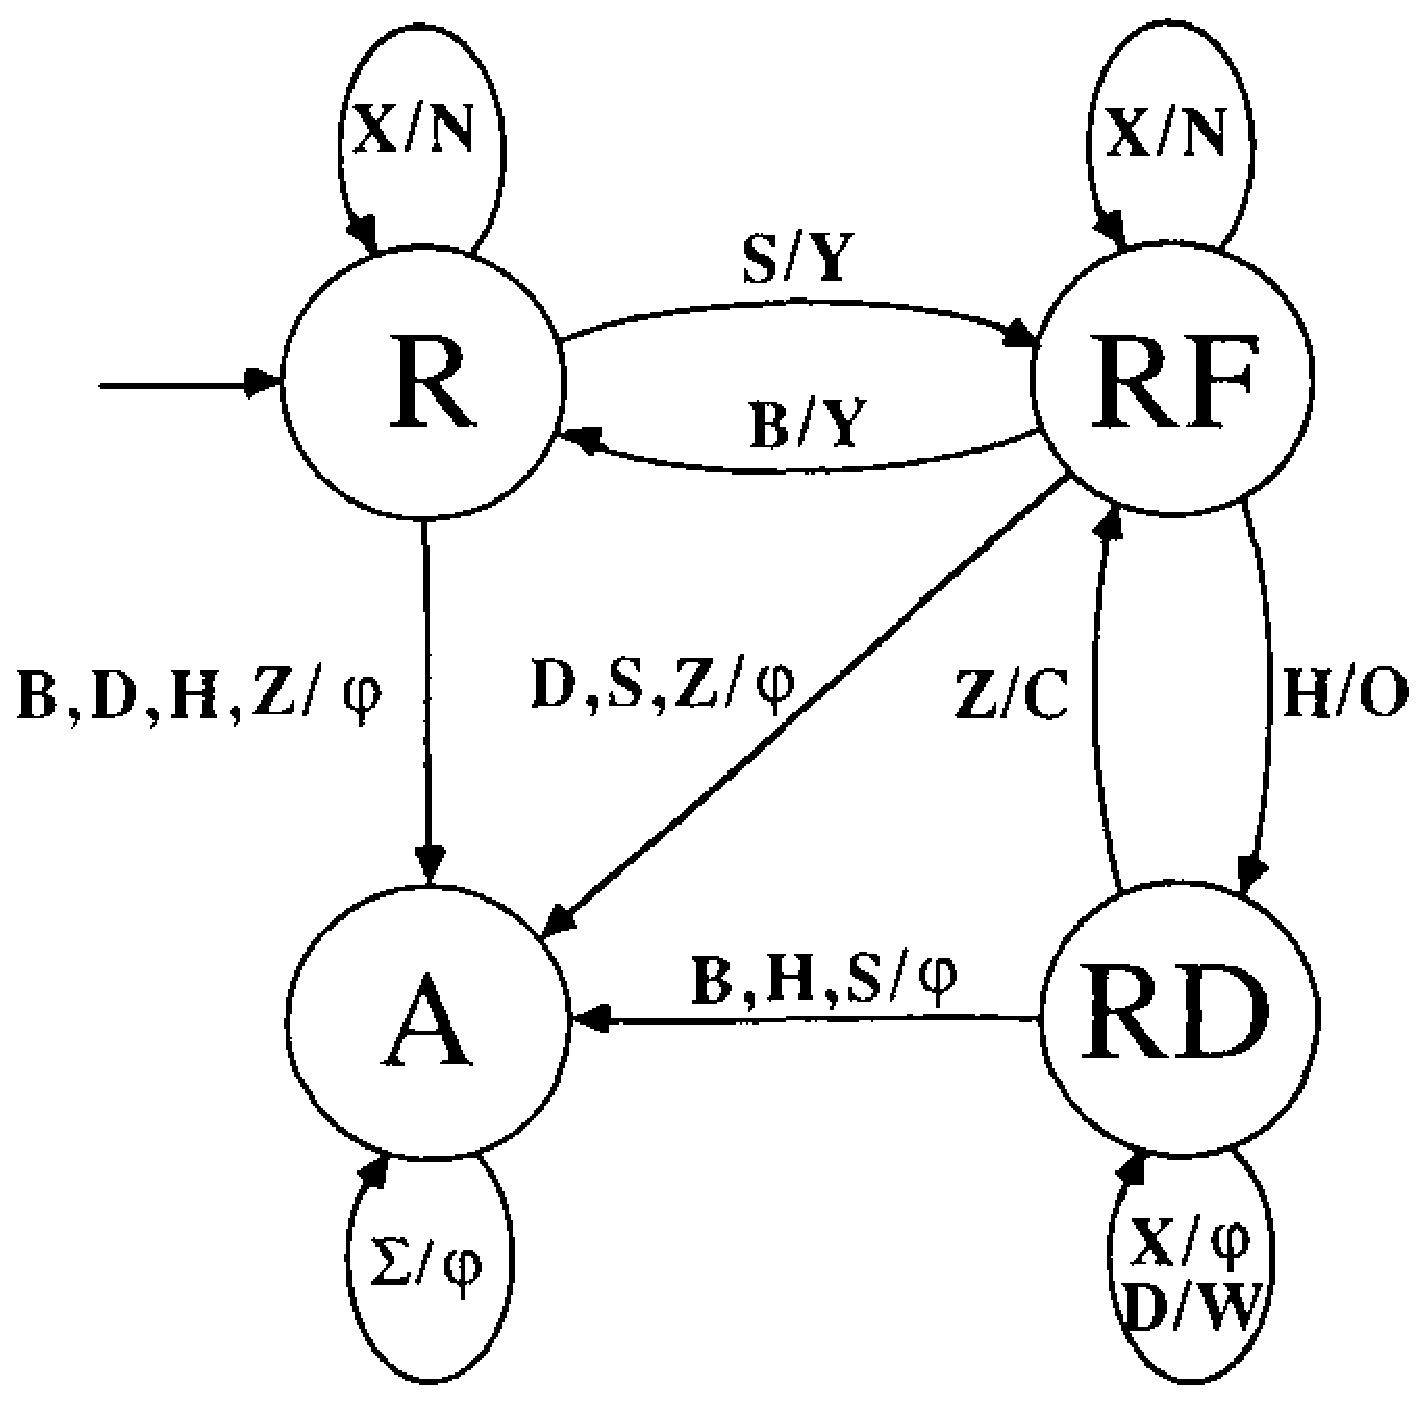
\epsfig{figure=ToFAfigures/fig7-10.eps,width=2.5in}}
\caption{The state transition diagram for the receive portion of Kermit, as
discussed in Example 7.14}\label{fig-7.10}
\end{figure}

\subsection*{Example 7.15}\index{addition automaton (FST)}

A computation such as the one shown in Figure \ref{fig-7.11}a would be divided up into
columns and presented to the FST as indicated in Figure \ref{fig-7.11}b (shown in
mid-computation). A digit from the first number and the corresponding digit from
the second number are presented to the transducer as a single input symbol. With
the column pairs represented by standard ordered pairs, the corresponding input
might appear as in Figure \ref{fig-7.12} (shown at the start of computation). As
illustrated by the orientation of the tape, this FST must be set up to process
strings \emph{in reverse}, that is, from right to left, since computations must
start with the low-order bits to ensure that the correct answer is always
(deterministically) computed. With states $C$ (representing carry) and $N$ (no
carry), input alphabet\index{binary alphabet} $\Sigma=\{\langle 0,0\rangle,\langle 0,1\rangle,\langle
1,0\rangle,\langle 1,1\rangle\}$ and output alphabet $\Gamma=\{\pmb{0},
\pmb{1}\}$, this binary adder behaves as shown in the state transition diagram
given for $B$ in Figure \ref{fig-7.13}. For the problem displayed in Figure \ref{fig-7.11}a, the
output produced by $B$ would be $\pmb{01001}$ (9 in binary), which is the
appropriate translation of the addition problem given ($6+3$).

% Figure 7.11
\begin{figure}
\centerline{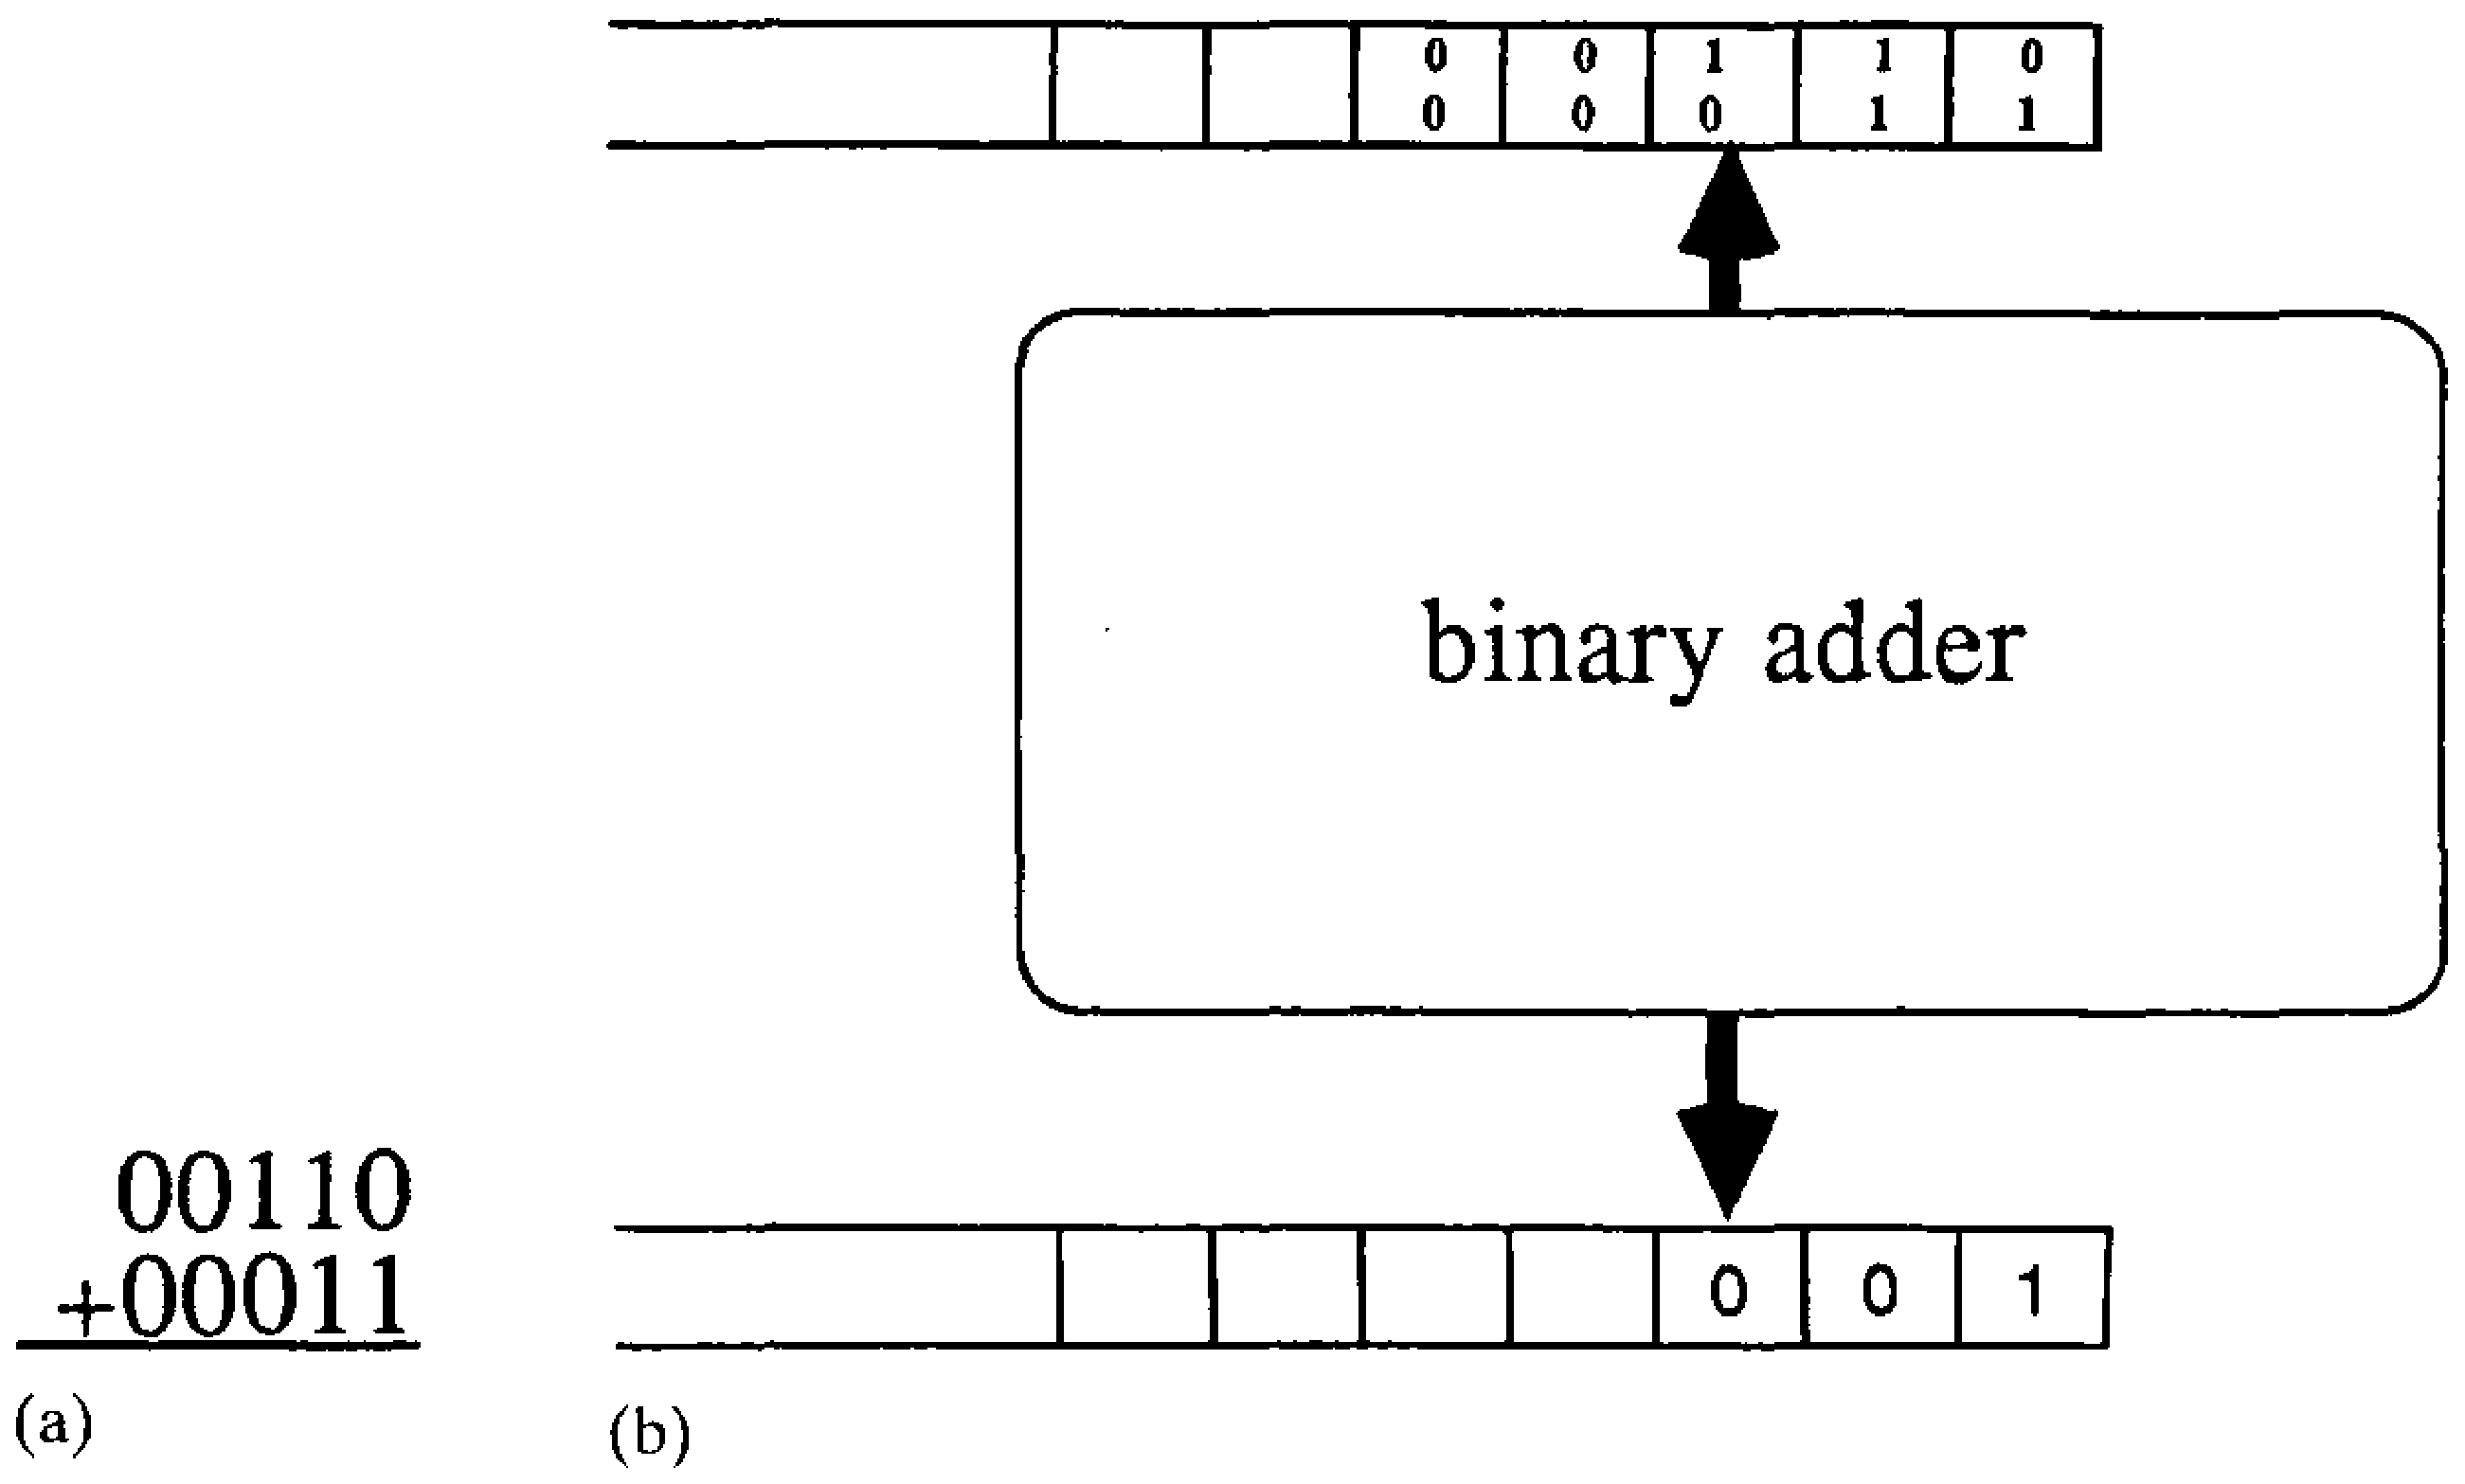
\epsfig{figure=ToFAfigures/fig7-11.eps,width=5.5in}}
\caption{(a) The addition problem discussed in Example 7.15 (b) Conceptual model
of the binary adder discussed in Example 7.15}\label{fig-7.11}
\end{figure}

% Figure 7.12
\begin{figure}
\centerline{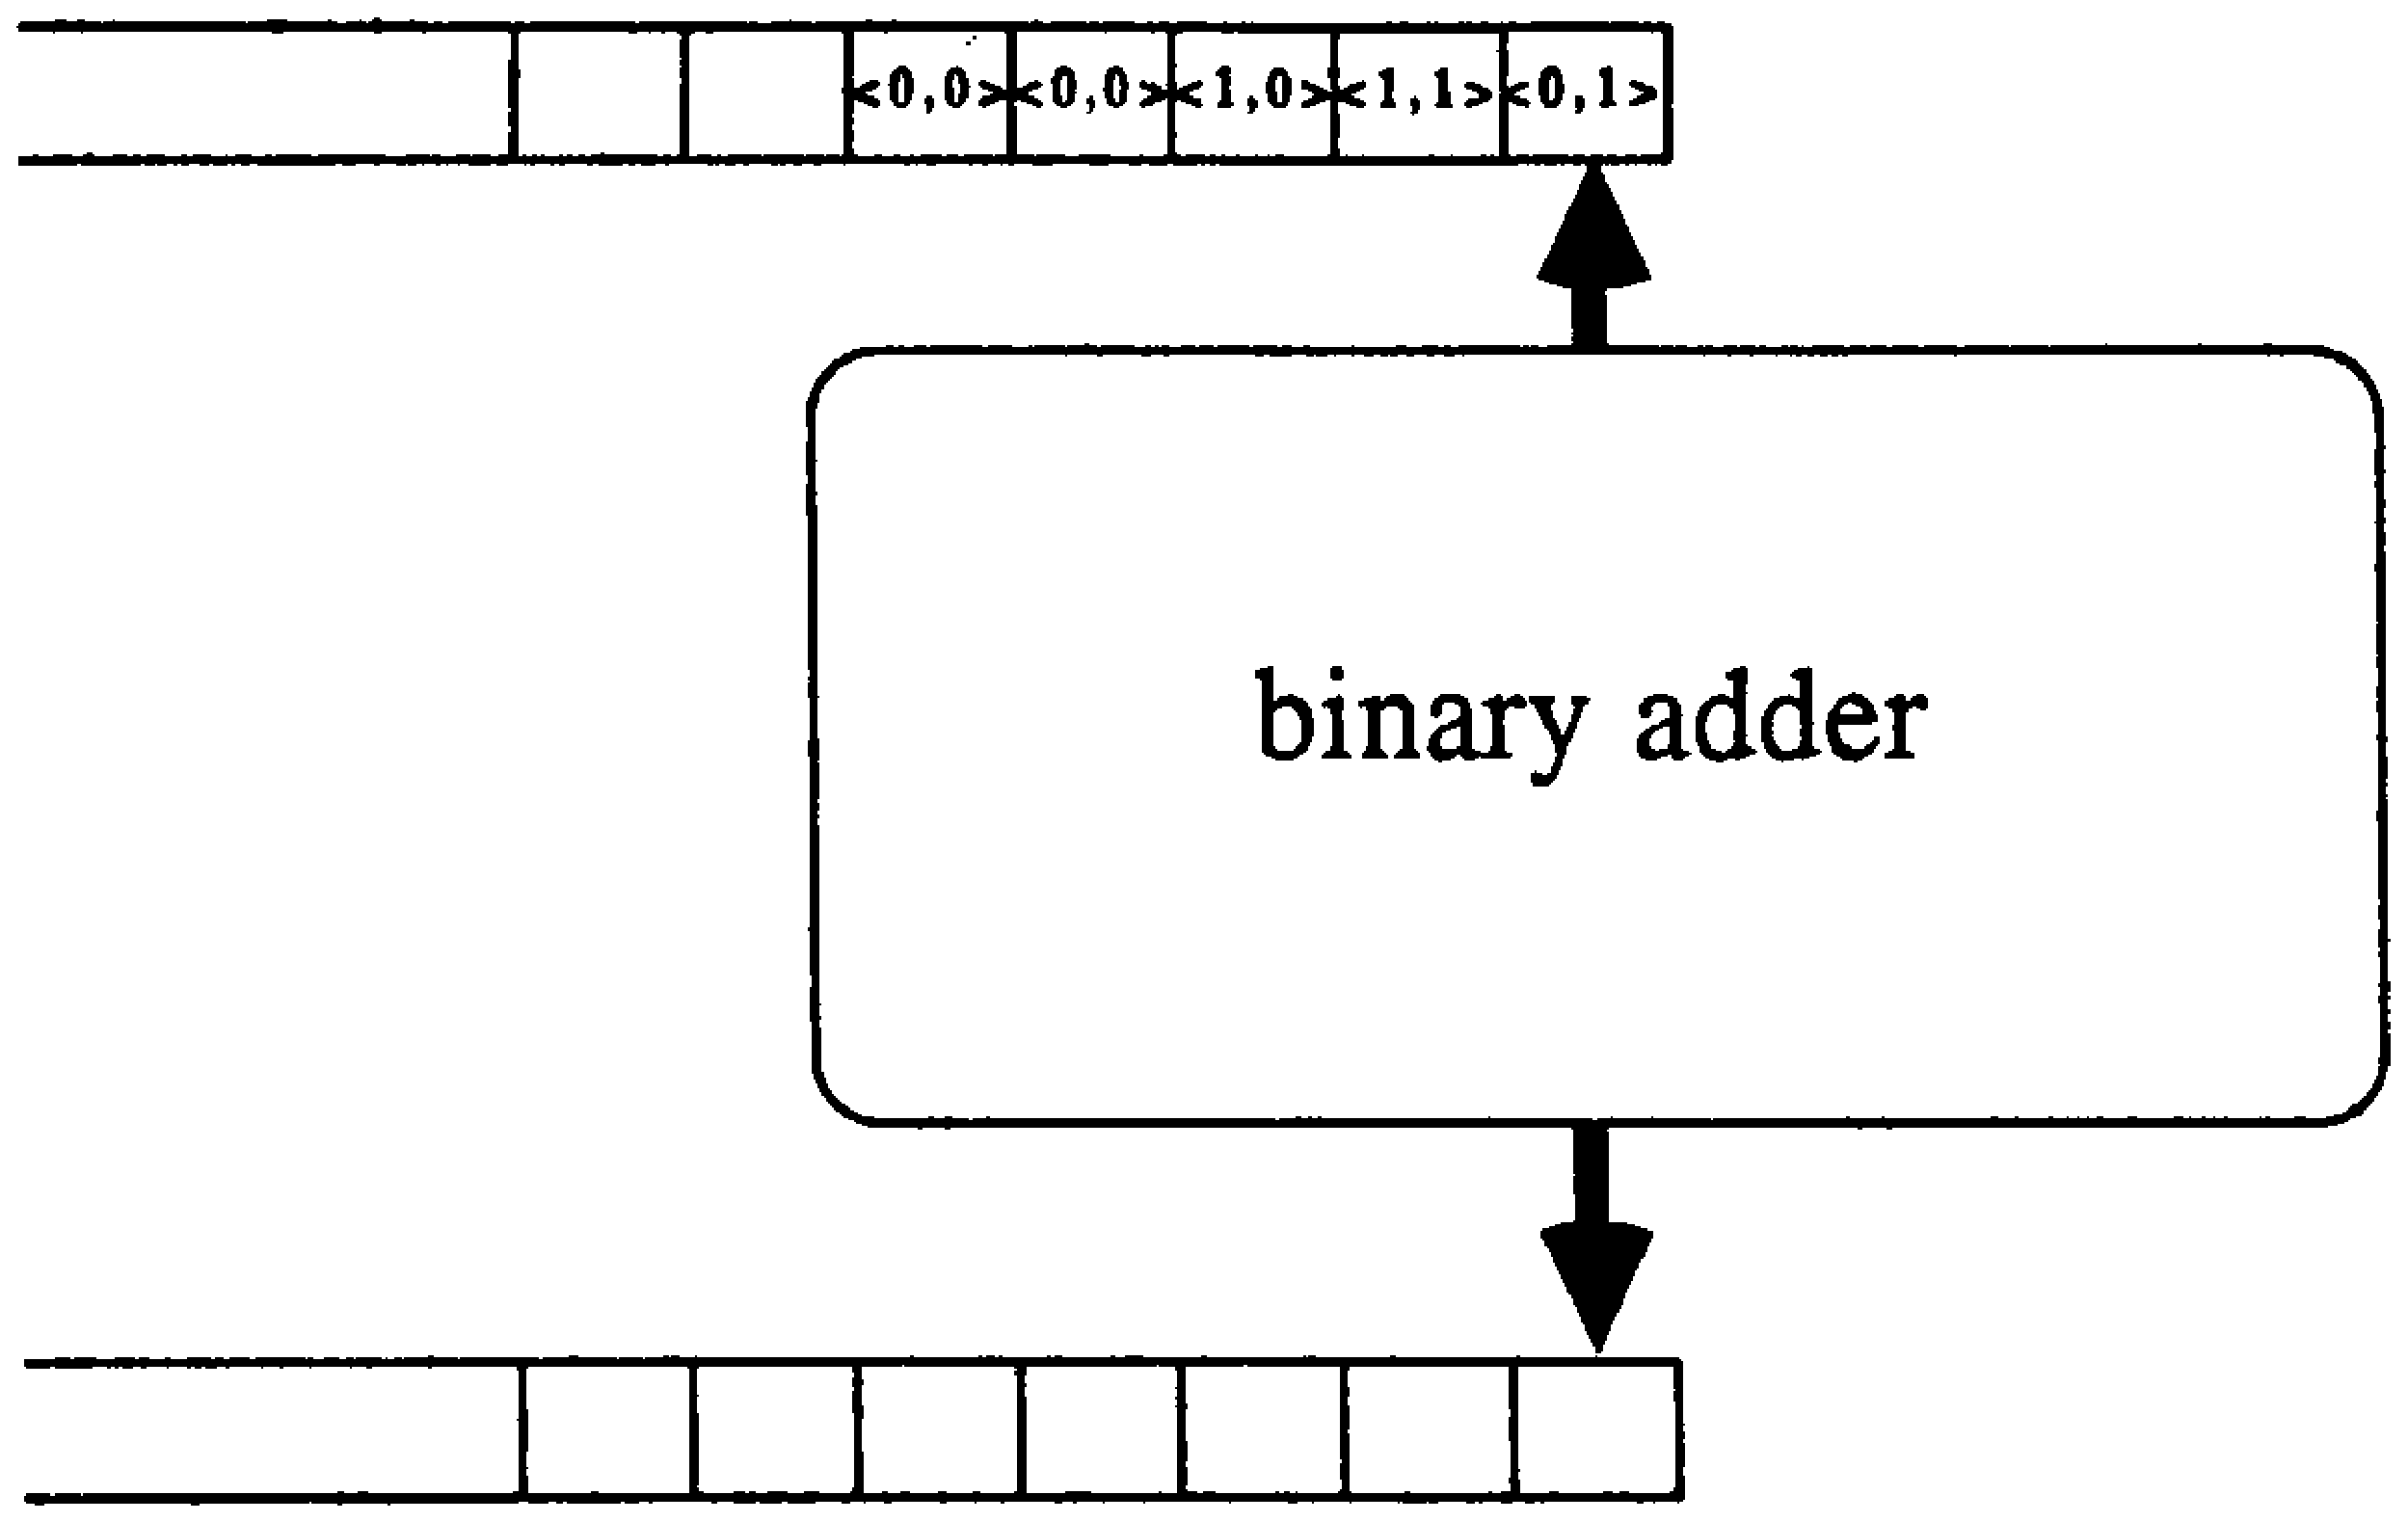
\epsfig{figure=ToFAfigures/fig7-12.eps,width=5.5in}}
\caption{The binary adder discussed in Example 7.15}\label{fig-7.12}
\end{figure}

Unfortunately, addition is not truly length preserving; adding the three-digit
numbers $\pmb{110}$ and $\pmb{011}$ produces a binary answer that is four digits
long. The adder $B$ defined in Example 7.15 cannot correctly reflect a carry out
of the most significant binary position. While the concept of final states is
not present in our formal definition of transducers, this FST $B$ provides an
example in which it is natural to both produce continuous output and track the
terminal state: if a computation ends in state $C$, then we know that an
overflow condition has occurred. $B$ clearly operates correctly on all strings
that have been padded with $\langle 0,0\rangle$ as the last (leftmost) symbol;
employing such padding is reminiscent of the use of the \<EOS\> symbol when
building circuits for DFAs. Indeed, it might be profitable to specifically
include an \<EOS\> symbol and have the transducer react to \<EOS\> by printing a
$\pmb{y}$ or $\pmb{n}$ to indicate whether or not there was overflow.

% Figure 7.13
\begin{figure}
\centerline{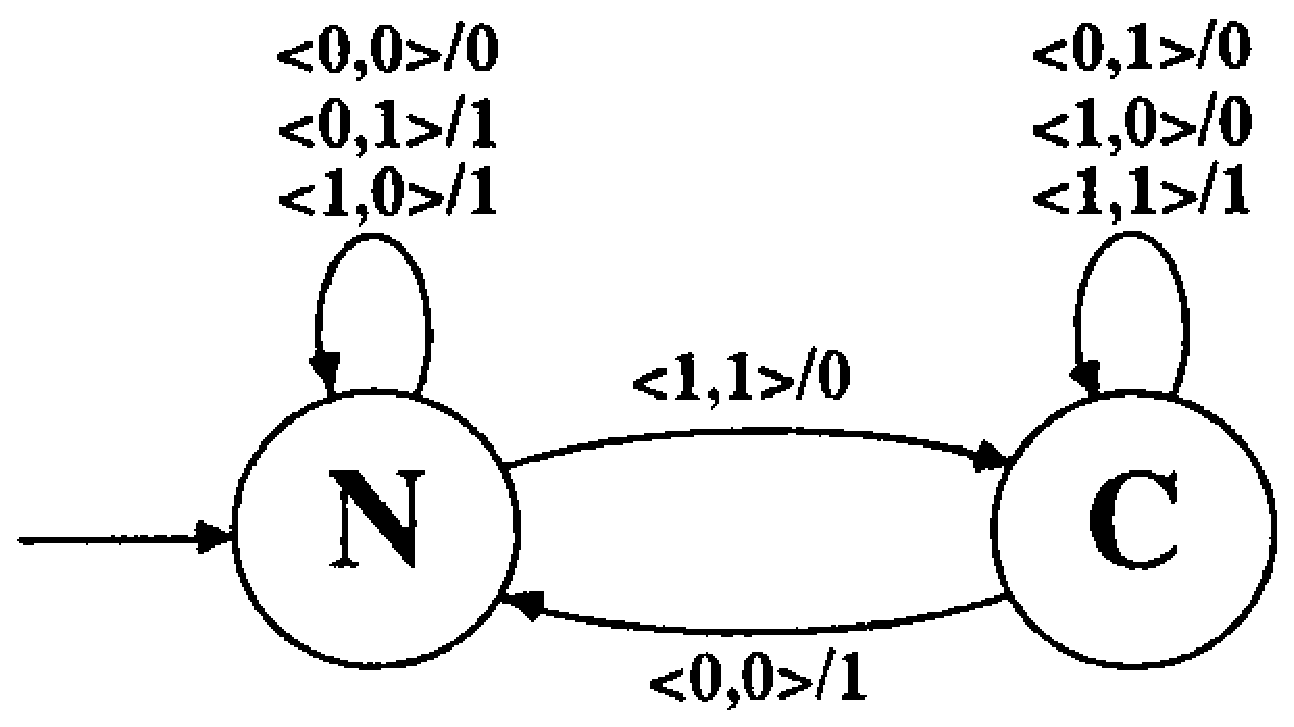
\epsfig{figure=ToFAfigures/fig7-13.eps,width=2.5in}}
\caption{The state transition diagram for a binary adder modeled as a Mealy
machine, as discussed in Example 7.15}\label{fig-7.13}
\end{figure}

While the binary adder is only one small component of a computer, finite-state
transducers can be profitably used to model complete systems; one such
application involves traffic lights. The controller for a large intersection
may handle eight banks of traffic signals for the various straight-ahead and
left-turn lanes, as well as four sets of walk lights (see the exercises). Input
about the intersection conditions is often fed to the controller from pedestrian
walk buttons and metal detectors embedded in the roadway. For simplicity, we
will choose a simplified intersection to illustrate how to model a traffic
controller by a transducer. The simplified example nevertheless incorporates all
the essential features of the more intricate intersections. A full-blown model
would only require larger alphabets and more states.

\subsection*{Example 7.16}

Consider a small north-south street that terminates as it meets a large
east-west avenue, as shown in Figure \ref{fig-7.14}. Due to the heavy traffic along the
avenue, the westbound traffic attempting to turn left is governed by a left-turn
signal (signal 2 in Figure \ref{fig-7.14}). Traffic continuing west is controlled by
signal 1, while signal 3 governs eastbound traffic. Vehicles entering the
intersection from the south rely on signal 4. The red, yellow, and green lights
of these four signals represent the output of the transducer. Protecting
westbound traffic while turning left is accomplished by an output configuration
of $\langle G,G,R,R\rangle$, which is meant to indicate that the first two
signals are green while the eastbound and northbound lanes have red lights. The
output alphabet can thus be represented by ordered foursomes of $R,\ Y$, and $G$
(red, yellow, and green). We can succinctly define
\[ \Gamma=\{R,Y,G\} \times \{R,Y,G\} \times \{R,Y,G\} \times \{R,Y,G\}, \]
though there will be some combinations (like $\langle G,G,G,G\rangle$) that are
not expected to appear in the model.

% Figure 7.14
\begin{figure}
\centerline{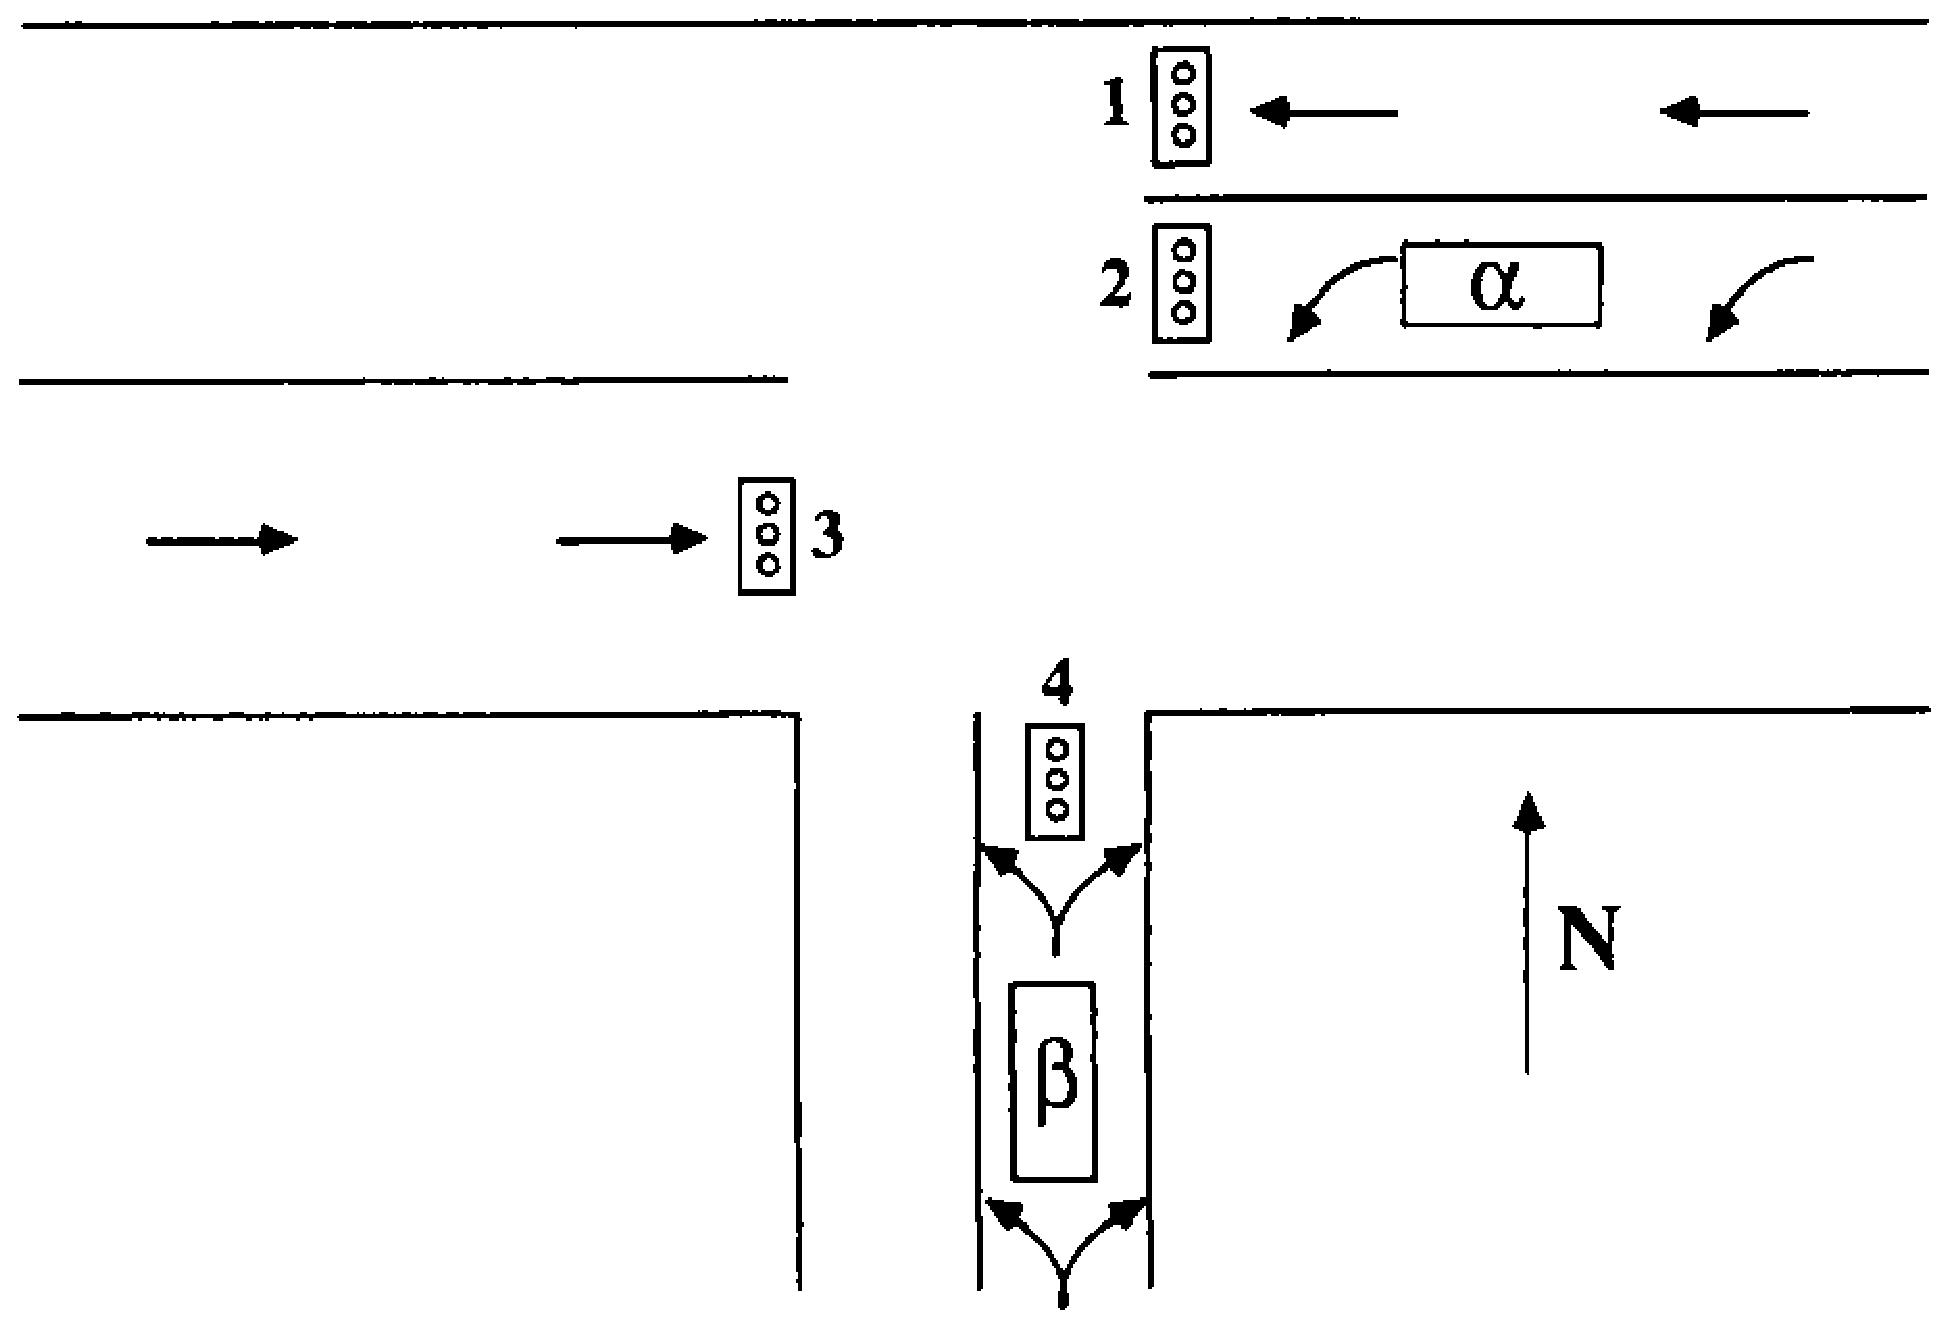
\epsfig{figure=ToFAfigures/fig7-14.eps,width=3.5in}}
\caption{The intersection discussed in Example 7.16}\label{fig-7.14}
\end{figure}

The most prevalent output configuration is expected to be $\langle
G,R,G,R\rangle$, which allows unrestricted flow of the east-west traffic on the
avenue. Due to the relatively small amount of traffic on the north-south street,
the designers of the intersection chose to embed the sensors $\alpha$ in the
left-turn lane and $\beta$ in the northbound lane and only depart from the
$\langle G,R,G,R\rangle$ configuration when a vehicle is sensed by these
detectors. There is therefore a pair of inputs to our transducer, indicating the
status of sensor $\alpha$ and sensor $\beta$. The four combinations will be
represented by $\langle 0,0\rangle$, (no traffic above either sensor), $\langle
1,0\rangle$ (sensor $\alpha$ active), $\langle 0,1\rangle$ (sensor $\beta$
active), and $\langle 1,1\rangle$ (both detectors have currently sensed
vehicles).

The controller is most naturally modeled by a Moore machine, since the state
of the system is so intimately tied to the status of the four lights. From the
configuration $\langle G,R,G,R\rangle$, activation of the $\beta$ sensor
signifies that all traffic should be stopped except that governed by signal 4.
The output should therefore move through the pattern $\langle Y,R,Y,R\rangle$ to
$\langle R,R,R,G\rangle$ and remain in that state until the $\beta$ sensor is
deactivated. This and the other transitions are illustrated in Figure \ref{fig-7.15}.

% Figure 7.15
\begin{figure}
\centerline{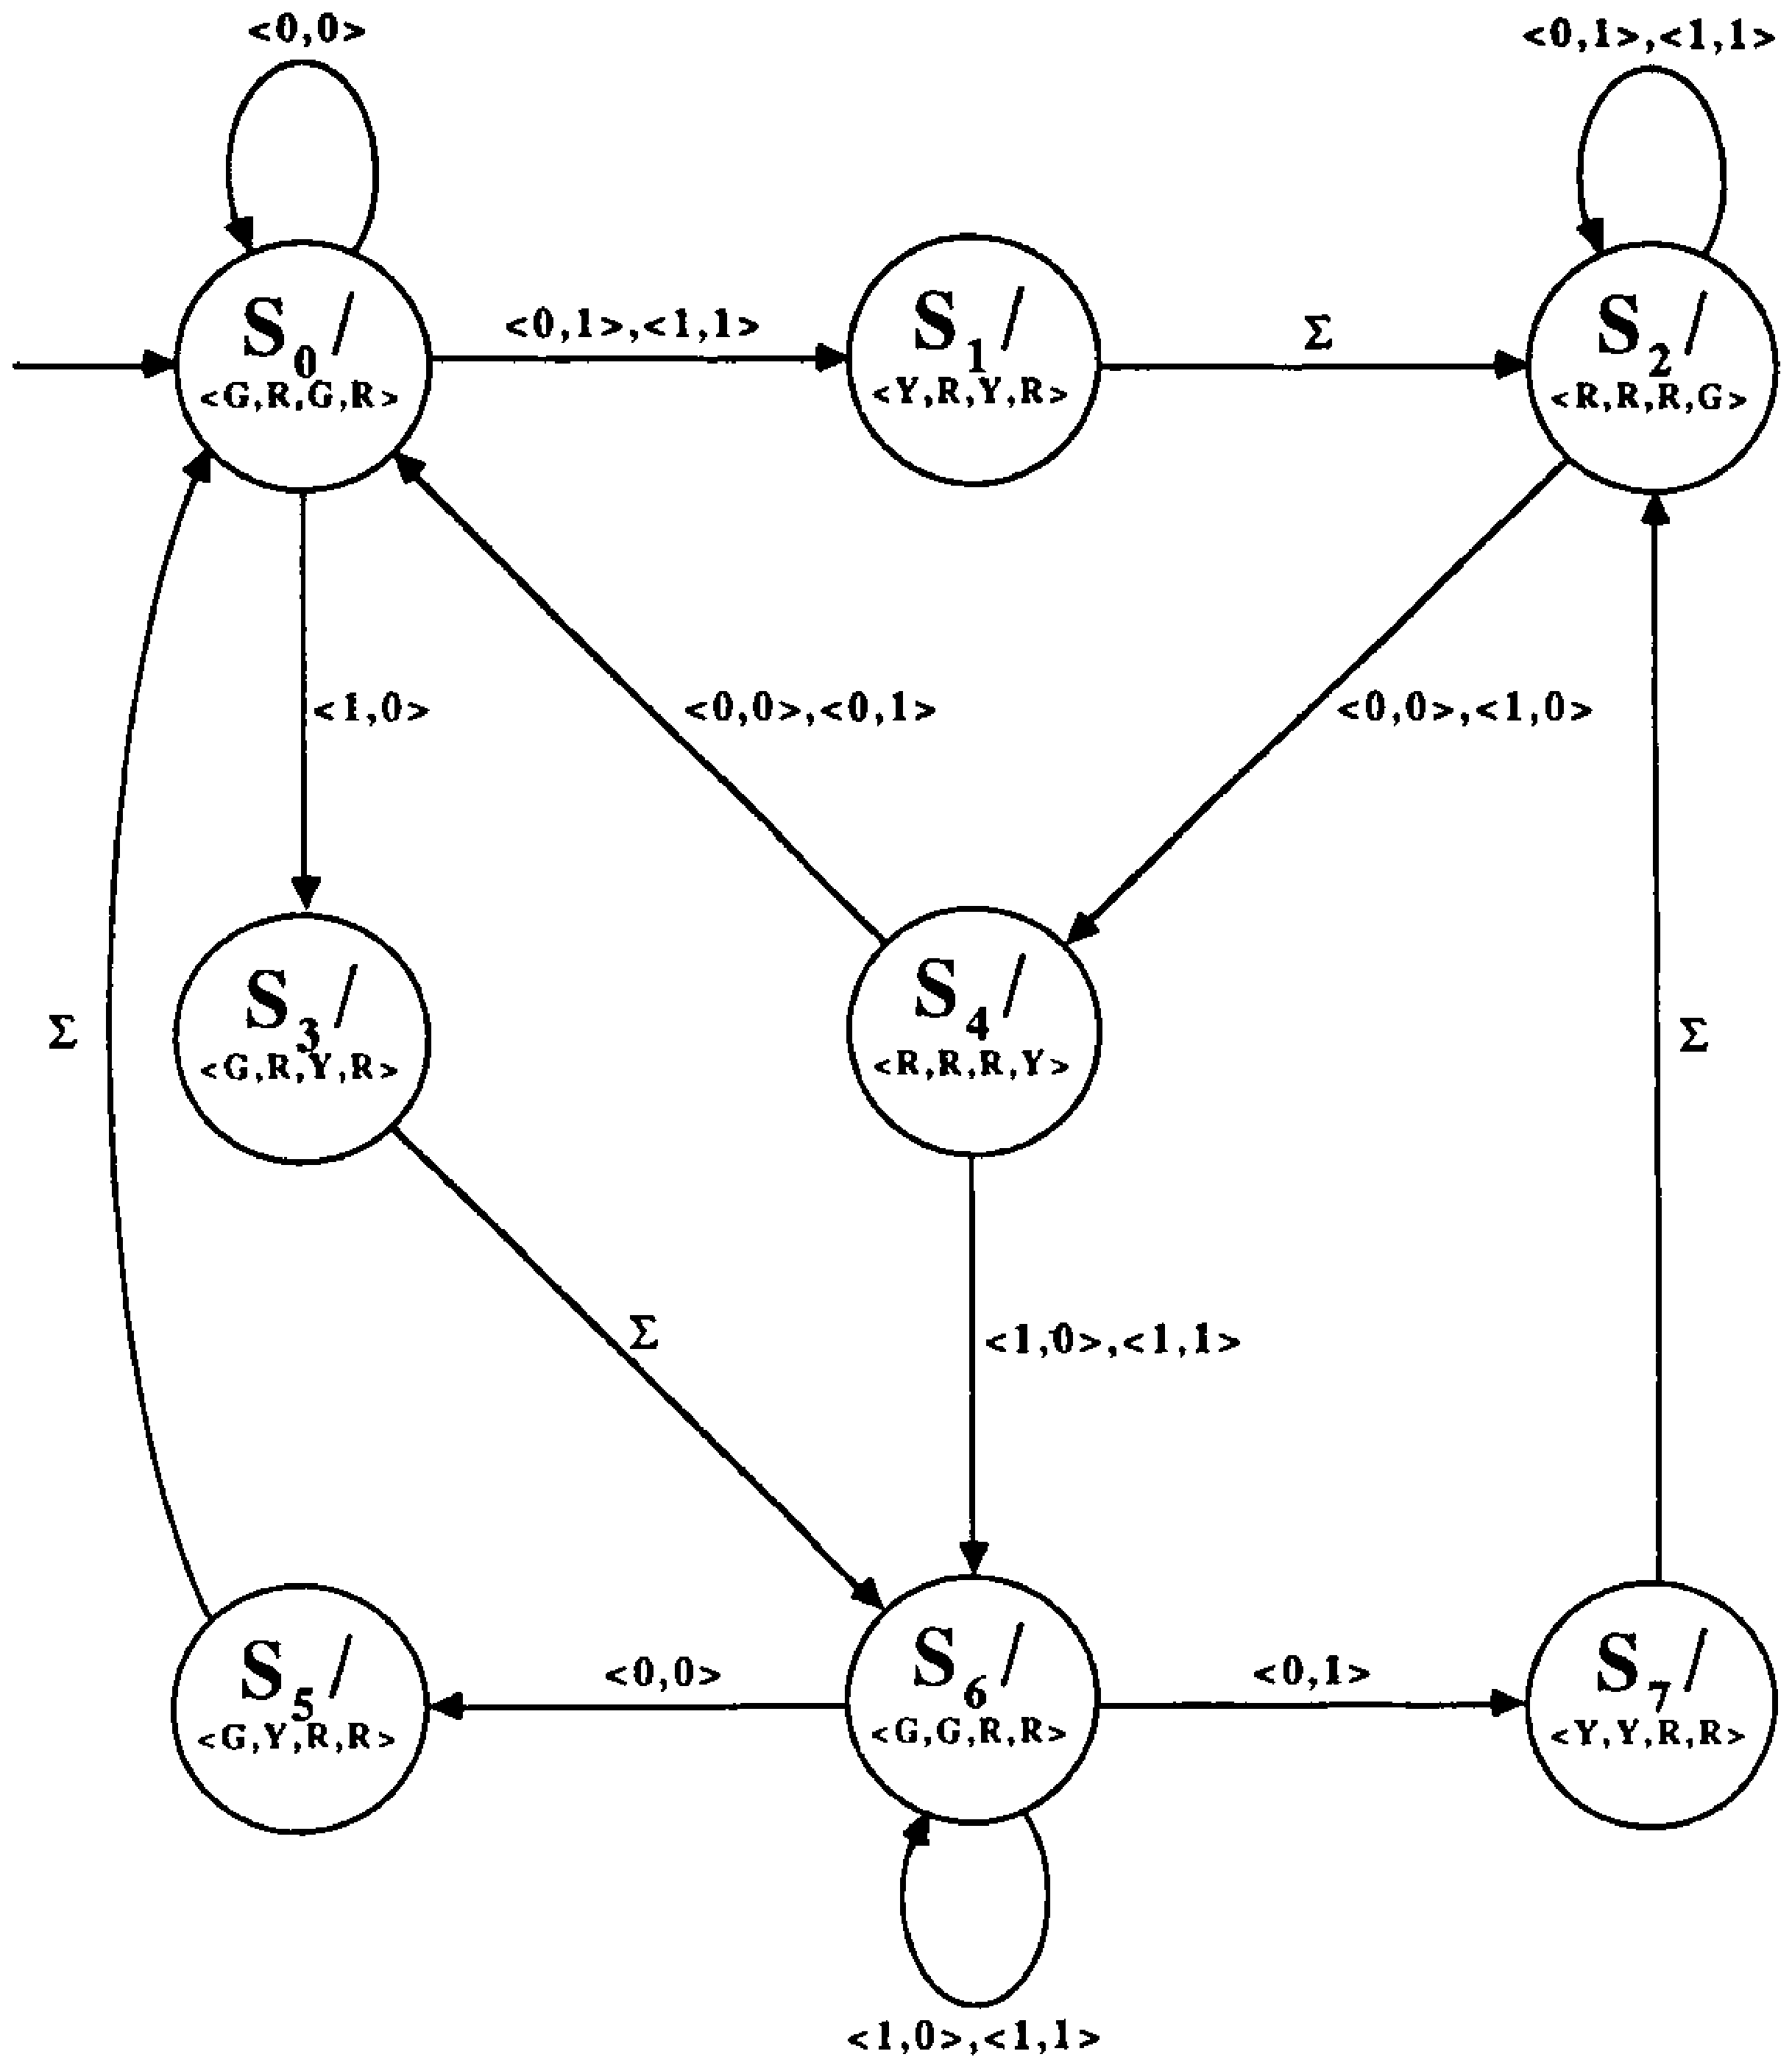
\epsfig{figure=ToFAfigures/fig7-15.eps,width=3.5in}}
\caption{The state transition diagram for a stoplight modeled as a
Moore machine, as discussed in Example 7.16}\label{fig-7.15}
\end{figure}

In actuality, the duration of patterns incorporating the yellow caution light
is shorter than others. With the addition of extra states, a clock cycle length
on the order of 5 seconds (commensurate with the typical length of a yellow
light) could be used to govern the length of the different output configurations.
For example, incorporating $s_g$ as shown in Figure \ref{fig-7.16} guarantees that the
output $\langle R,R,R,G\rangle$ will persist for at least two cycles (10
seconds). From an engineering standpoint, complicating the finite-state control
in this manner can be avoided by varying the clock cycle length.

% Figure 7.16
\begin{figure}
\centerline{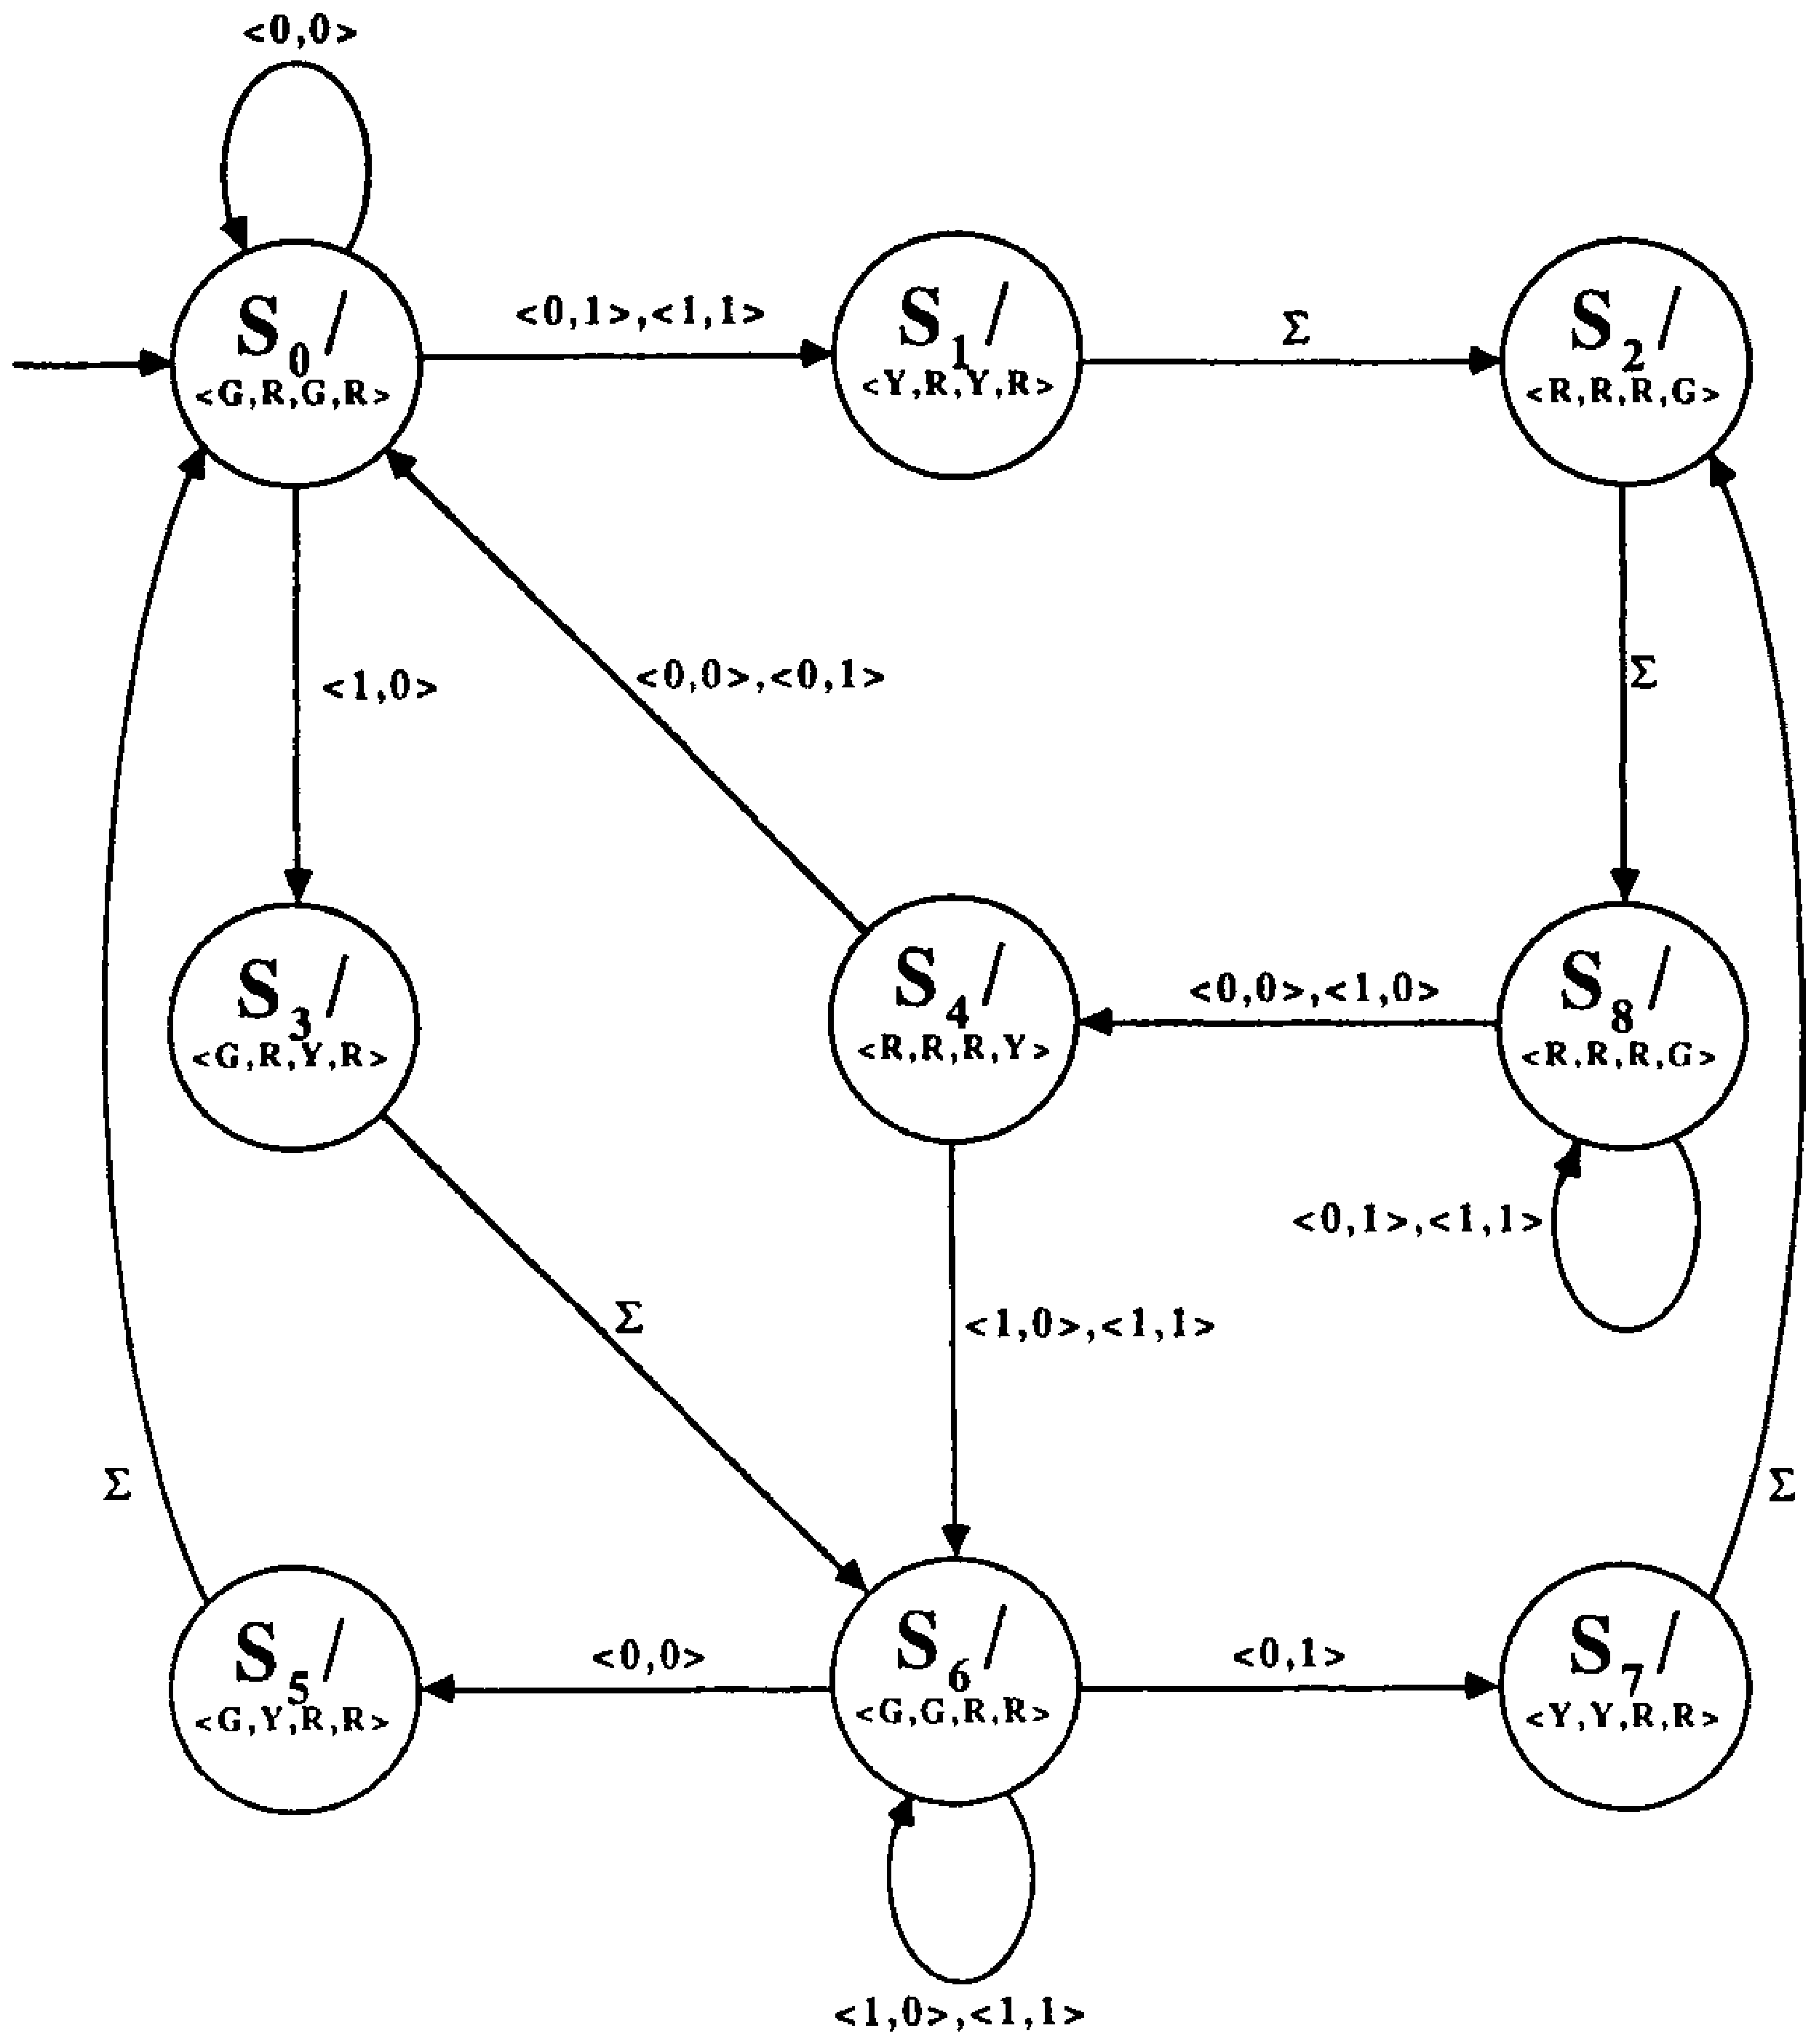
\epsfig{figure=ToFAfigures/fig7-16.eps,width=3.0in}}
\caption{The modified controller discussed in Example 7.16}\label{fig-7.16}
\end{figure}

We now discuss some of the hardware that comprise the heart of traffic
controllers and vending machines. As was done with deterministic finite
automata in Chapter \ref{ch-1} and nondeterministic finite automata in Chapter \ref{ch-4},
finite-state transducers can be implemented with digital logic circuits. We
again use a clock pulse, D flip-flops, and an encoding for the states. Besides
needing an encoding for the input alphabet, it is now necessary to have an
encoding for the output alphabet, which will be represented by the bits
$w_1,w_2,w_3,\ldots$. We again suggest (solely for simplicity and
standardization in the exercises) ordering the symbols in $\Gamma$
alphabetically and assigning binary codes in ascending order, as was recommended
earlier for $\Sigma$. We must construct a circuit for generating each $w_j$, in
the same manner as we built circuits implementing the accept function for finite
automata.

Many practical applications of FSTs (such as traffic signals) operate
continuously, rather than starting and stopping for one small string. In such
cases, an \<EOS\> symbol is not necessary; the circuit operates until power is
shut off. Similarly, an \<SOS\> symbol is not essential for a traffic signal
complex; upon resuming operation after a power failure, it is usually immaterial
whether east-west traffic first gets a green light or whether it gets a red
light in deference to the north-south traffic. In contrast, it is important for
vending machines to initialize to the proper state or some interesting discounts
could be obtained by playing with the power cord.

\subsection*{Example 7.17}

Consider the FST displayed in Figure \ref{fig-7.17}. If \<EOS\> and \<SOS\> is
unnecessary, then the input alphabet can be represented by a single bit $a_1$,
with $a_1=\pmb{0}$ representing $\pmb{c}$ and $a_1=\pmb{1}$ representing $\pmb{d}$.
Similarly, the output alphabet can be represented by a single bit $w_1$ with
$w_1=\pmb{0}$ representing $\pmb{a}$ and $w_1=\pmb{1}$ representing $\pmb{b}$. The
states can likewise be represented by a single bit $t_1$, with $t_1=\pmb{0}$
representing $s_0$ and $t_1=\pmb{1}$ representing $s_1$. As before, we can
construct a truth table to represent the state transition function, defining
$t'_1$ in terms of $t_1$ and $a_1$. The complete table is given in Table 7.5a.

% Figure 7.17
\begin{figure}
\centerline{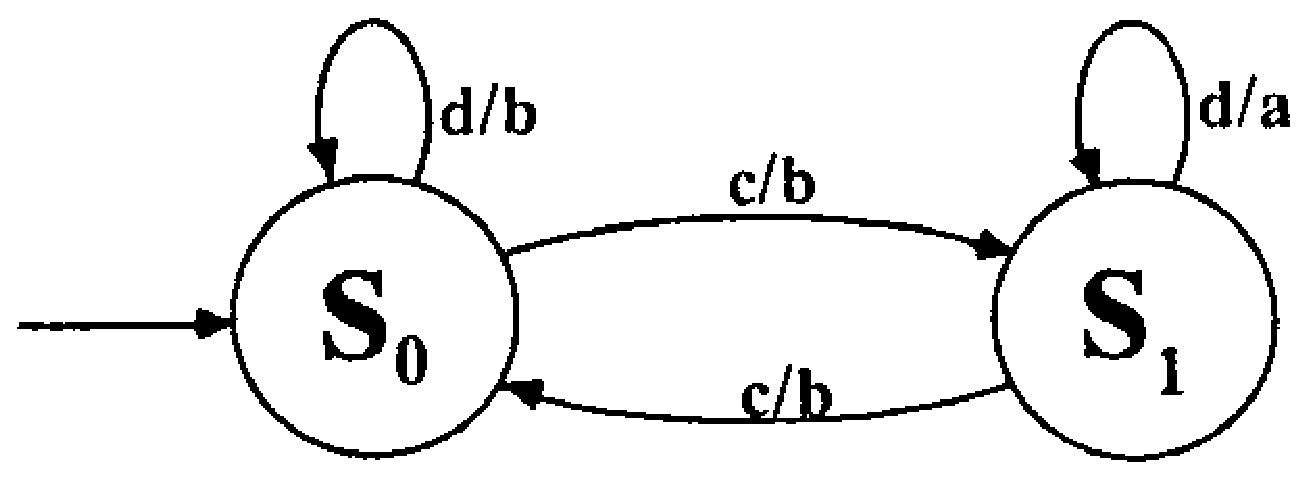
\epsfig{figure=ToFAfigures/fig7-17.eps,width=2.5in}}
\caption{The state transition diagram for the Mealy machine in Example 7.17}\label{fig-7.17}
\end{figure}

% Table 7.5a & 7.5b
\begin{table}\label{tbl-7.5}
\begin{center}
\begin{tabular}{cc|c}
\multicolumn{3}{c}{Table 7.5a} \\
$t_1$ & $a_1$ & $t'_1$ \\
\hline
$\pmb{1}$ & $\pmb{1}$ & $\pmb{1}$ \\
$\pmb{0}$ & $\pmb{1}$ & $\pmb{0}$ \\
$\pmb{1}$ & $\pmb{0}$ & $\pmb{0}$ \\
$\pmb{0}$ & $\pmb{0}$ & $\pmb{1}$
\end{tabular}
$\qquad$
\begin{tabular}{cc|c}
\multicolumn{3}{c}{Table 7.5b} \\
$t_1$ & $a_1$ & $w_1$ \\
\hline
$\pmb{1}$ & $\pmb{1}$ & $\pmb{0}$ \\
$\pmb{0}$ & $\pmb{1}$ & $\pmb{1}$ \\
$\pmb{1}$ & $\pmb{0}$ & $\pmb{1}$ \\
$\pmb{0}$ & $\pmb{0}$ & $\pmb{1}$
\end{tabular}
\end{center}
\end{table}

% Figure 7.18
\begin{figure}
\centerline{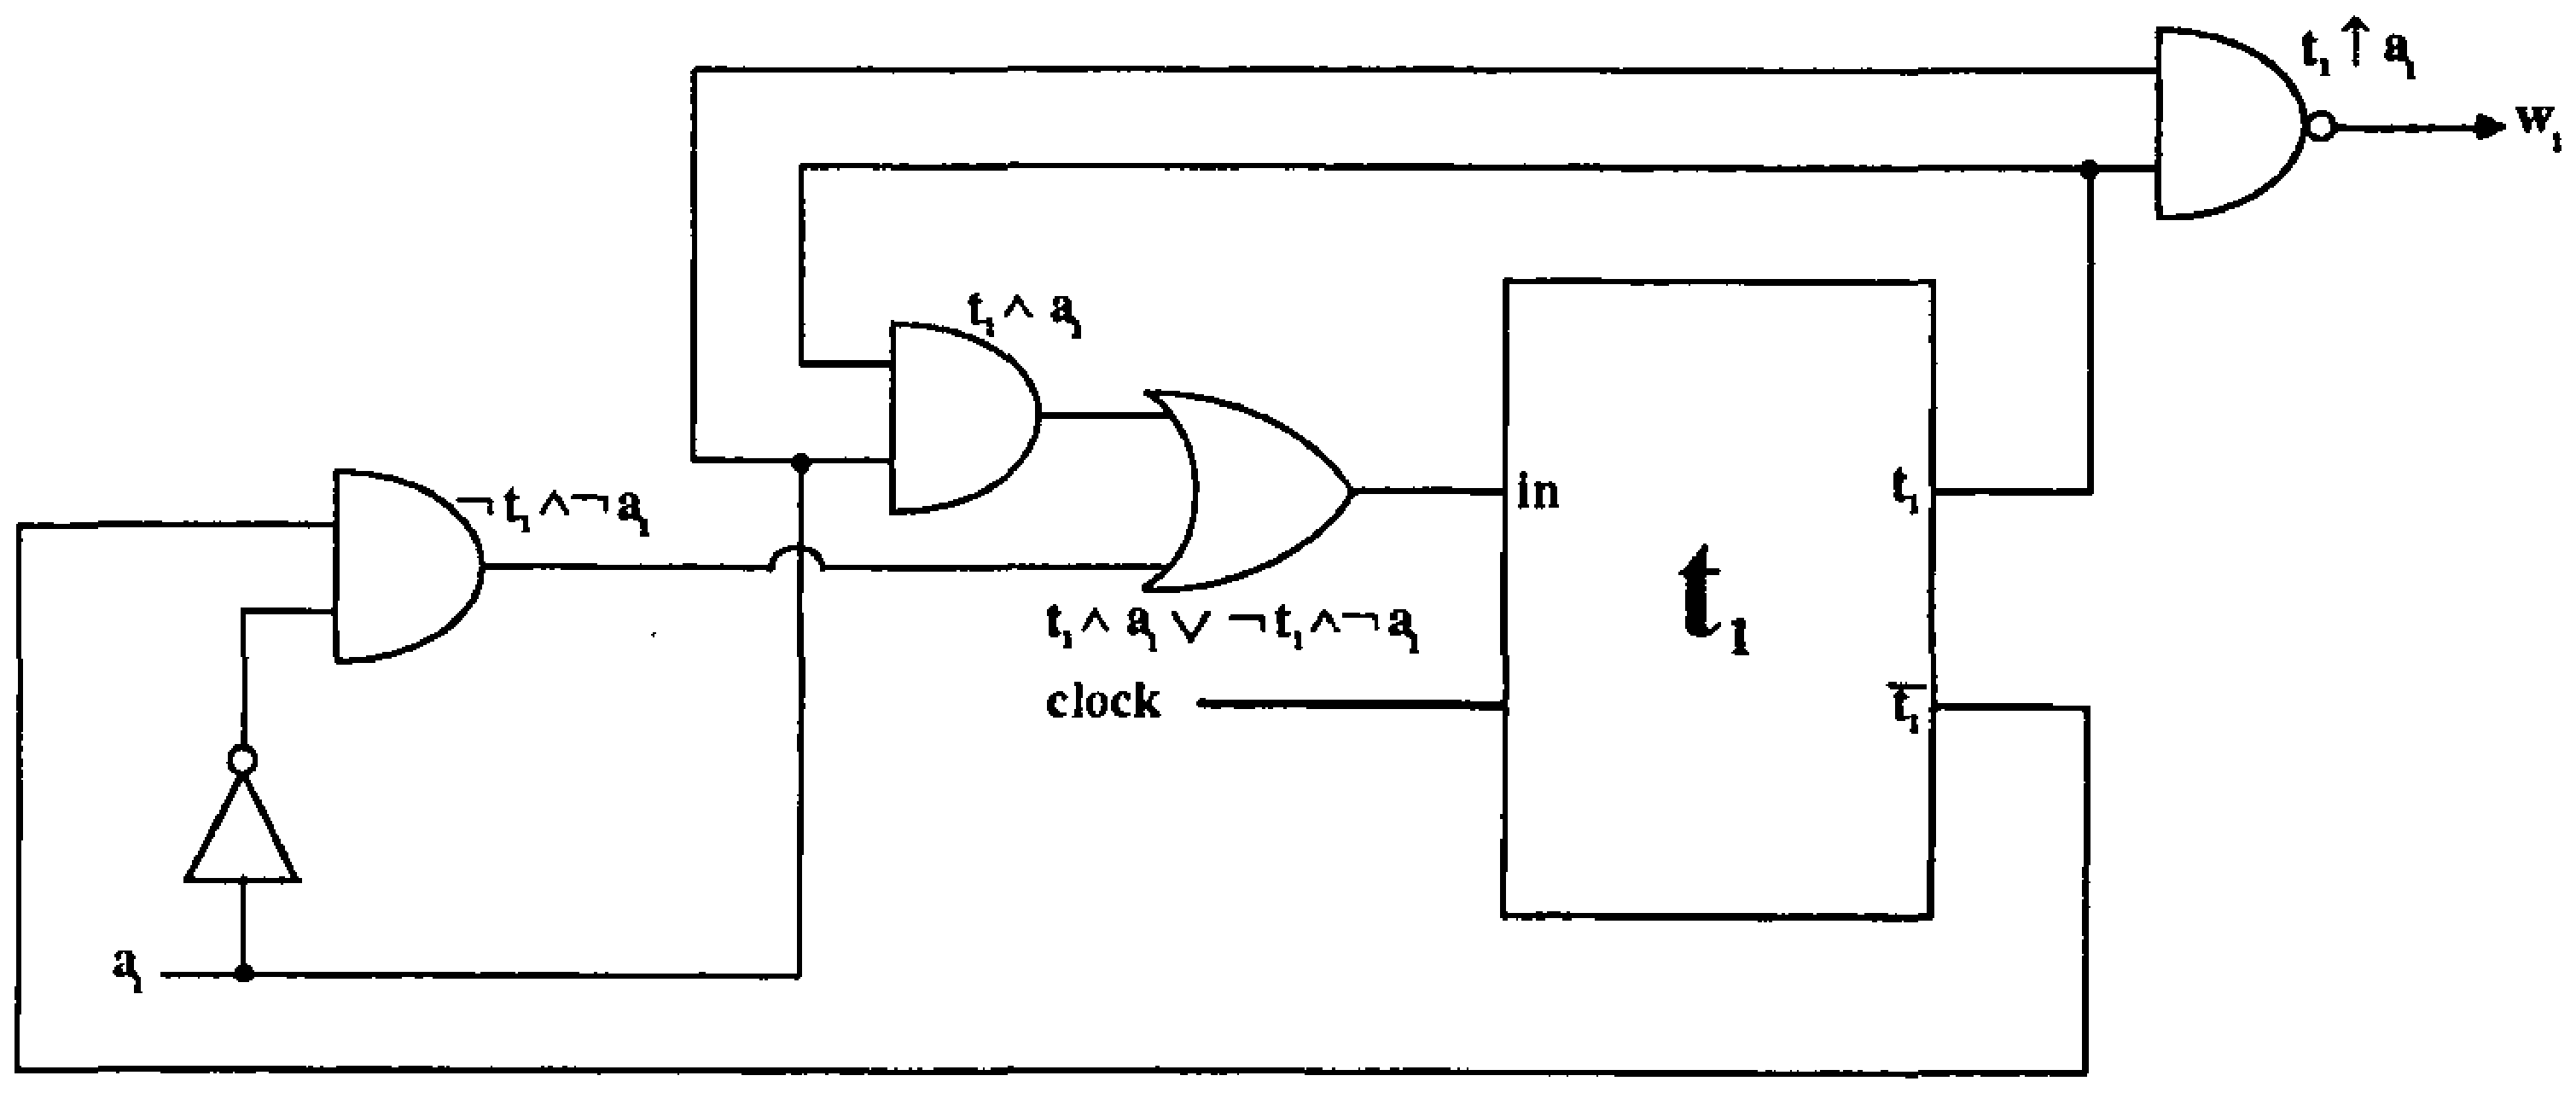
\epsfig{figure=ToFAfigures/fig7-18.eps,width=4.5in}}
\caption{Circuit diagram for Example 7.17}\label{fig-7.18}
\end{figure}

The principal disjunctive normal form for the transition function is therefore
seen to be $t'_1=(t_1 \wedge a_1)\vee(\neg t_1 \wedge \neg a_1)$. The output
function can be found in a similar manner, as shown in Table 7.5b.

Thus, $w_1=(t_1 \uparrow a_1)$. As in Example 1.12, the circuit for $t_1$, will
be fed back into the D flip-flop(s); the circuit for $w_1$ will form the output
for the machine (replacing the acceptance circuit used in DFAs). The complete
network is shown in Figure \ref{fig-7.18}. Note that we would want the output device to
print on the rising edge of the clock cycle, before the new value of $t_1$
propagates through the circuitry.

A larger output alphabet would require an encoding of several bits; each $w_1$
would have its own network of gates, and the complete circuit would then
simultaneously generate several bits of output information. As in Chapter \ref{ch-1},
additional states or input symbols will add bits to the other encoding schemes
and add to the number of rows in the truth tables for $\delta$ and $\omega$.
Each additional state bit will also require its own D flip-flop and a new truth
table for its feedback loop. Each additional state bit doubles the number of
states that can be represented, which means that, as was the case with
deterministic finite automata, the number of flip-flops grows as the logarithm
of the number of states.

\section*{Exercises}
\begin{enumerate}[{7.}1.]
\item Let $A=\langle\Sigma,\Gamma,S,s_0,\delta,\omega\rangle$ be a Mealy
machine. Prove the following statements from Theorem \ref{thm-7.1}:
\begin{enumerate}
\item $(\forall x \in \Sigma^*)(\forall y \in \Sigma^*)(\forall t \in S)
	(\OBAR(t,yx) = \OBAR(t,y) \cdot \OBAR(\DBAR(t,y),x))$
\item $(\forall x \in \Sigma^*)(\forall y \in \Sigma^*)(\forall s \in S)
	(\DBAR(s,yx) = \DBAR(\DBAR(s,y),x))$
\end{enumerate}

\item Refer to Lemma \ref{lmm-7.1} and prove:
\begin{enumerate}
\item $(\forall s \in S_A)(\forall x \in \Sigma^*)(\mu(\DBAR_A(s,x)) =
	\DBAR_B(\mu(s),x))$
\item $(\forall s \in S_A)(\forall x \in \Sigma^*)(\OBAR_A(s,x) =
	\OBAR_B(\mu(s),x))$
\end{enumerate}

\item Prove Corollary \ref{cor-7.3}.

\item Prove Corollary \ref{cor-7.4} by showing that a necessary and sufficient condition
for a Mealy machine $M$ to be minimal is that $M$ is both reduced and connected.

\item Show that any FTD function $f$ must satisfy a ``pumping lemma.''
\begin{enumerate}
\item Devise the statement of a theorem that shows that the way any sufficiently
long string is translated determines how an entire sequence of longer strings
are translated.
\item Prove the statement made in part (a).
\end{enumerate}

\item In each of the following parts, you may assume the results in the
preceding parts; for example, you may assume parts (a) and (b) when proving (c).
\begin{enumerate}
\item Prove Lemma \ref{lmm-7.3}a.
\item Prove Lemma \ref{lmm-7.3}b.
\item Prove Lemma \ref{lmm-7.3}c.
\item Prove Lemma \ref{lmm-7.3}d.
\item Prove Lemma \ref{lmm-7.3}e.
\end{enumerate}

\item Given a FST $M=\langle\Sigma,\Gamma,S,s_0,\delta,\omega\rangle$, prove the
following statements from Lemma \ref{lmm-7.4}:
\begin{enumerate}
\item $E_{0M}$ has just one equivalence classes, which consists of all of $S$.
\item $E_{1M}$ is defined by $s E_{1M} t \Leftrightarrow (\forall \pmb{a} \in \Sigma)
	(\omega(s,\pmb{a}) = \omega(t,\pmb{a}))$.
\item $(\forall s \in S)(\forall t \in S)(\forall i \geq 1)(s E_{i+1M} t
	\Leftrightarrow s E_{iM} t \wedge (\forall\pmb{a}\in\Sigma)
	(\delta(s,\pmb{a}) E_{iM} \delta(t,\pmb{a}))$.
\end{enumerate}

\item Prove Theorem \ref{thm-7.6} by showing that if $A=\langle\Sigma,\Gamma,S,s_0,\delta,
\omega\rangle$ is a Moore machine then \[(\forall x \in \Sigma^*)(\forall y \in
\Sigma^*)(\forall t \in S)(\OBAR(t,yx) = \OBAR(t,y) \cdot \OBAR(\DBAR(t,y),x))\]

\item Prove Theorem \ref{thm-7.7}.

\item Prove Theorem \ref{thm-7.8}.

\item Use Lemma \ref{lmm-7.6} to find $E_C$ in Example 7.10.

\item Show that there is a homomorphism from the machine $M$ in Example 7.11 to
the machine $B$ in Example 7.2.

\item Prove that, in a FST $M=\langle\Sigma,\Gamma,S,s_0,\delta,\omega\rangle,\ 
(\forall t \in S)(\forall\pmb{a}\in\Sigma)(\OBAR(t,\pmb{a})=\omega(t,\pmb{a}))$.

\item Modify the vending machine in Example 7.1 so that it can return all the
coins that have been inserted. Let $\pmb{r}$ denote a new input that represents
activating the coin return, and let $\pmb{a}$ represent a new output corresponding
to the vending machine releasing all the coins in its temporary holding area.

\item Given a FST $M=\langle\Sigma,\Gamma,S,s_0,\delta,\omega\rangle$ and
$M/\!\!_{E_M}=\langle\Sigma,\Gamma,S_{E_M},s_{0_{E_M}},\delta_{E_M},\omega_{E_M}
\rangle$, show that $\delta_{E_M}$ is well defined.

\item Given a FST $M=\langle\Sigma,\Gamma,S,s_0,\delta,\omega\rangle$ and
$M/\!\!_{E_M}=\langle\Sigma,\Gamma,S_{E_M},s_{0_{E_M}},\delta_{E_M},\omega_{E_M}
\rangle$, show that $\omega_{E_M}$ is well defined.

\item Give an example that shows that requiring a FST $M$ to be reduced is not a
sufficient condition to ensure that $M$ is minimal.

\item Show that the function $\mu$ defined in the proof of Theorem \ref{thm-7.5} is well
defined.

\item Given the function $\mu$ defined in the proof of Theorem \ref{thm-7.5}, prove that
$\mu$ is really an isomorphism; that is:
\begin{enumerate}
\item $\mu(s_{0_1}) = s_{0_2}$
\item $(\forall s \in S_1)(\forall a \in \Sigma)(\mu(\delta_1(s,\pmb{a})) =
	\delta_2(\mu(s),\pmb{a}))$
\item $(\forall s \in S_1)(\forall\pmb{a}\in\Sigma)(\omega_1(s,\pmb{a}) =
	\omega_2(\mu(s),\pmb{a}))$
\item $\mu$ is a one-to-one function between $S_1$ and $S_2$.
\item $\mu$ is onto $S_2$.
\end{enumerate}

\item Consider a transducer that implements a ``one-unit delay'' over the
alphabets $\Sigma=\{\pmb{a},\pmb{b}\}$ and $\Gamma=\{\pmb{a},\pmb{b},\pmb{x}\}$.
The first letter of the output string should be $\pmb{x}$, and the $n$th letter of
the output string should be the $n - 1$st letter of the input string (for
$n>1$). Thus, $\OBAR(\pmb{abbab})=\pmb{xabba}$, and so on.
\begin{enumerate}
\item Define a sextuple for a Mealy machine that will perform this translation.
\item Draw a Mealy machine that will perform this translation.
\item Define a sextuple for a Moore machine that will perform this translation.
\item Draw a Moore machine that will perform this translation.
\end{enumerate}

\item Consider the circuit diagram that would correspond to the vending machine
in Example 7.1.
\begin{enumerate}
\item Does there appear to be any reason to use an \<EOS\> symbol in the input
alphabet? Explain.
\item Does there appear to be any reason to use an \<SOS\> symbol in the input
alphabet? Explain.
\item How many encoding bits are needed for the input alphabet? Define an
appropriate encoding scheme.
\item How many encoding bits are needed for the output alphabet? Define an
appropriate encoding scheme.
\item How many encoding bits are needed for the state names? Define an
appropriate encoding scheme.
\item Write the truth table and corresponding (minimized) Boolean function for
$t_2$. Try to make the best possible use of the don't-care combinations.
\item Write the truth table and corresponding (minimized) Boolean function for
$w_2$. Try to make the best possible use of the don't-care combinations.
\item Define the other functions and draw the complete circuit for the vending
machine.
\end{enumerate}

\item Consider the vending machine described in Exercise 7.14.
\begin{enumerate}
\item Does there appear to be any reason to use an \<EOS\> symbol in the input
alphabet? Explain.
\item How many encoding bits are needed for the input alphabet? Define an
appropriate encoding scheme.
\item How many encoding bits are needed for the output alphabet? Define an
appropriate encoding scheme.
\item How many encoding bits are needed for the state names? Define an
appropriate encoding scheme.
\item Write the truth table and corresponding (minimized) Boolean function for
$t_3$ Try to make the best possible use of the don't-care combinations.
\item Write the truth table and corresponding (minimized) Boolean function for
$w_3$. Try to make the best possible use of the don't-care combinations.
\item Define the other functions and draw the complete circuit for the vending
machine.
\end{enumerate}

\item Use the standard encoding conventions to draw the circuit corresponding
to the FST defined in Example 7.2.

\item Use the standard encoding conventions to draw the circuit corresponding
to the FST defined in Example 7.6.

\item Use the standard encoding conventions to draw the circuit corresponding
to the FST $D$ defined in Example 7.8.

\item Give an example that shows that requiring a FST $M$ to be connected is not
a sufficient condition to ensure that $M$ is minimal.

\item Consider a transducer that implements a ``two-unit delay'' over the
alphabets $\Sigma=\{\pmb{a},\pmb{b}\}$ and $\Gamma=\{\pmb{a},\pmb{b},\pmb{x}\}$.
The first two letters of the output string should be $\pmb{xx}$, and the $n$th
letter of the output string should be the $n-2$nd letter of the input string
(for $n > 2$). Thus, $\OBAR(\pmb{abbaba})=\pmb{xxabba}$, and so on.
\begin{enumerate}
\item Define a sextuple for a Mealy machine that will perform this translation.
\item Draw a Mealy machine that will perform this translation.
\item Define a sextuple for a Moore machine that will perform this translation.
\item Draw a Moore machine that will perform this translation.
\end{enumerate}

\item \begin{enumerate}
\item Give an example that shows that the conclusion of Theorem \ref{thm-7.5} can be
false if $M_1$ is not reduced.
\item What essential property of the proposed isomorphism $\mu$ is now absent?
\end{enumerate}

\item \begin{enumerate}
\item Give an example that shows that the conclusion of Theorem \ref{thm-7.5} can be
false if $M_1$ is not connected.
\item What essential property of the proposed isomorphism $\mu$ is now absent?
\end{enumerate}

\item \begin{enumerate}
\item Give an example that shows that the conclusion of Theorem \ref{thm-7.5} can be
false if $M_2$ is not reduced.
\item What essential property of the proposed isomorphism $\mu$ is now absent?
\end{enumerate}

\item \begin{enumerate}
\item Give an example that shows that the conclusion of Theorem \ref{thm-7.5} can be
false if $M_2$ is not connected.
\item What essential property of the proposed isomorphism $\mu$ is now absent?
\end{enumerate}

\item \begin{enumerate}
\item Give an example of a FST $A$ for which $A$ is \emph{not} reduced and $A'$
is not reduced.
\item Give an example of a FST $A$ for which $A$ is \emph{not} reduced and $A'$
\emph{is} reduced.
\end{enumerate}

\item Complete the proof of Theorem \ref{thm-7.4} by showing:
\begin{enumerate}
\item $(\forall y \in \Sigma^*)(\forall t \in S)(\OBAR(t,y) =
	\OBAR_{E_M}([t]_{E_M},y))$.
\item $M/\!\!_{E_M}$ is equivalent to $M$.
\item $M/\!\!_{E_M}$ is reduced.
\item If $M$ is connected, then $M/\!\!_{E_M}$ is connected.
\end{enumerate}

\item Let $\Sigma=\{\pmb{0},\pmb{1}\}$ and $\Gamma=\{\pmb{y},\pmb{n}\}$.
\begin{enumerate}
\item Define $f_1(\pmb{a}_1\pmb{a}_2\ldots \pmb{a}_m)=y^m$ if $\pmb{a}_1=
\pmb{1}$, and let $f_1(\pmb{a}_1\pmb{a}_2\ldots a^m) = n^m$ otherwise. Thus,
$f_1(\pmb{10})=\pmb{yy}$ and $f_1(\pmb{0101})=\pmb{nnnn}$. Demonstrate that
$f_1$ is FTD.
\item Define $f_2(\pmb{a}_1\pmb{a}_2\ldots \pmb{a}_m)=y^m$ if $\pmb{a}_m=
\pmb{1}$, and let $f_2(\pmb{a}_2\pmb{a}_2\ldots \pmb{a}_m)=n^m$ otherwise. Thus,
$f_2(\pmb{10})=\pmb{nn}$ and $f_2(\pmb{0101})=\pmb{yyyy}$. Prove that $f_2$ is
\emph{not} FTD.
\end{enumerate}

\item Let $\Sigma=\{\pmb{a},\pmb{b}\}$ and $\Gamma=\{\pmb{0},\pmb{1}\}$. Define
$f_3(\pmb{a}_1\pmb{a}_2\ldots a_m)$ to be the first $m$ letters of the infinite
sequence $\pmb{010010001000010^510^610^710^81}\ldots$. Thus,
$f_3(\pmb{ababababab})=\pmb{0100100010}$ and $f_3(\pmb{abbaa})=\pmb{01001}$.
Argue that $f_3$ is \emph{not} FTD.

\item Assume $f$ is FTD. Prove that $(\forall x \in \Sigma^n)(\forall y \in
\Sigma^*)(\forall z \in \Sigma^*)$ (the first $n$ letters of $f(xy)$ must agree
with the first $n$ letters of $f(xz)$).

\item Consider an elevator in a building with two floors. Floor one has an up
button $\pmb{u}$ on the wall, floor two has a down button $\pmb{d}$, and there are
buttons labeled $\pmb{1}$ and $\pmb{2}$ inside the elevator itself. The four actions
taken by the elevator are close the doors, open the doors, go to floor 1, and go
to floor 2. Assume that an inactive elevator will attempt to close the doors.
For simplicity, assume that the model is not to incorporate sensors to test for
improperly closed doors, nor are there buttons to hold the doors open, and the
like. Also assume that when the elevator arrives on a given floor the call
button for that floor is automatically deactivated (rather than modeling the
shutoff as a component of the output).
\begin{enumerate}
\item Define the input alphabet for this transducer (compare with Example 7.16).
\item Define the output alphabet for this transducer.
\item Define the Mealy sextuple that will model this elevator.
\item Draw a Mealy machine that will model this elevator.
\item Define the Moore sextuple that will model this elevator.
\item Draw a Moore machine that will model this elevator.
\item Without using \<EOS\> or \<SOS\>, draw a circuit that will implement the
transducer defined in part (d).
\end{enumerate}

\item Build a Mealy machine that will serve as a traffic signal controller for
the intersection described in Example 7.16.

\item Consider the intersection described in Example 7.16 with walk signals
added to the north-south crosswalks (only). As shown in Figure \ref{fig-7.19}, there is an
additional input sensor $\gamma$ corresponding to the pedestrian walk button and
an additional component of the output that will always be in one of two states
($\pmb{W}$ for walk and $\pmb{D}$ for don't walk). There are walk buttons at each of
the corners, but they all trip the same single input sensor; similarly, the
output for the walk light is displayed on each corner, but they all change at
once and can be modeled as a single component. Assume that if the walk button is
activated all traffic but that on the side street is stopped, and the walk
lights change from $\pmb{D}$ to $\pmb{W}$. Further assume that the walk lights
revert to $\pmb{D}$ and $\pmb{W}$ before the side street light turns to yellow.
% Figure 7.19
\begin{figure}
\centerline{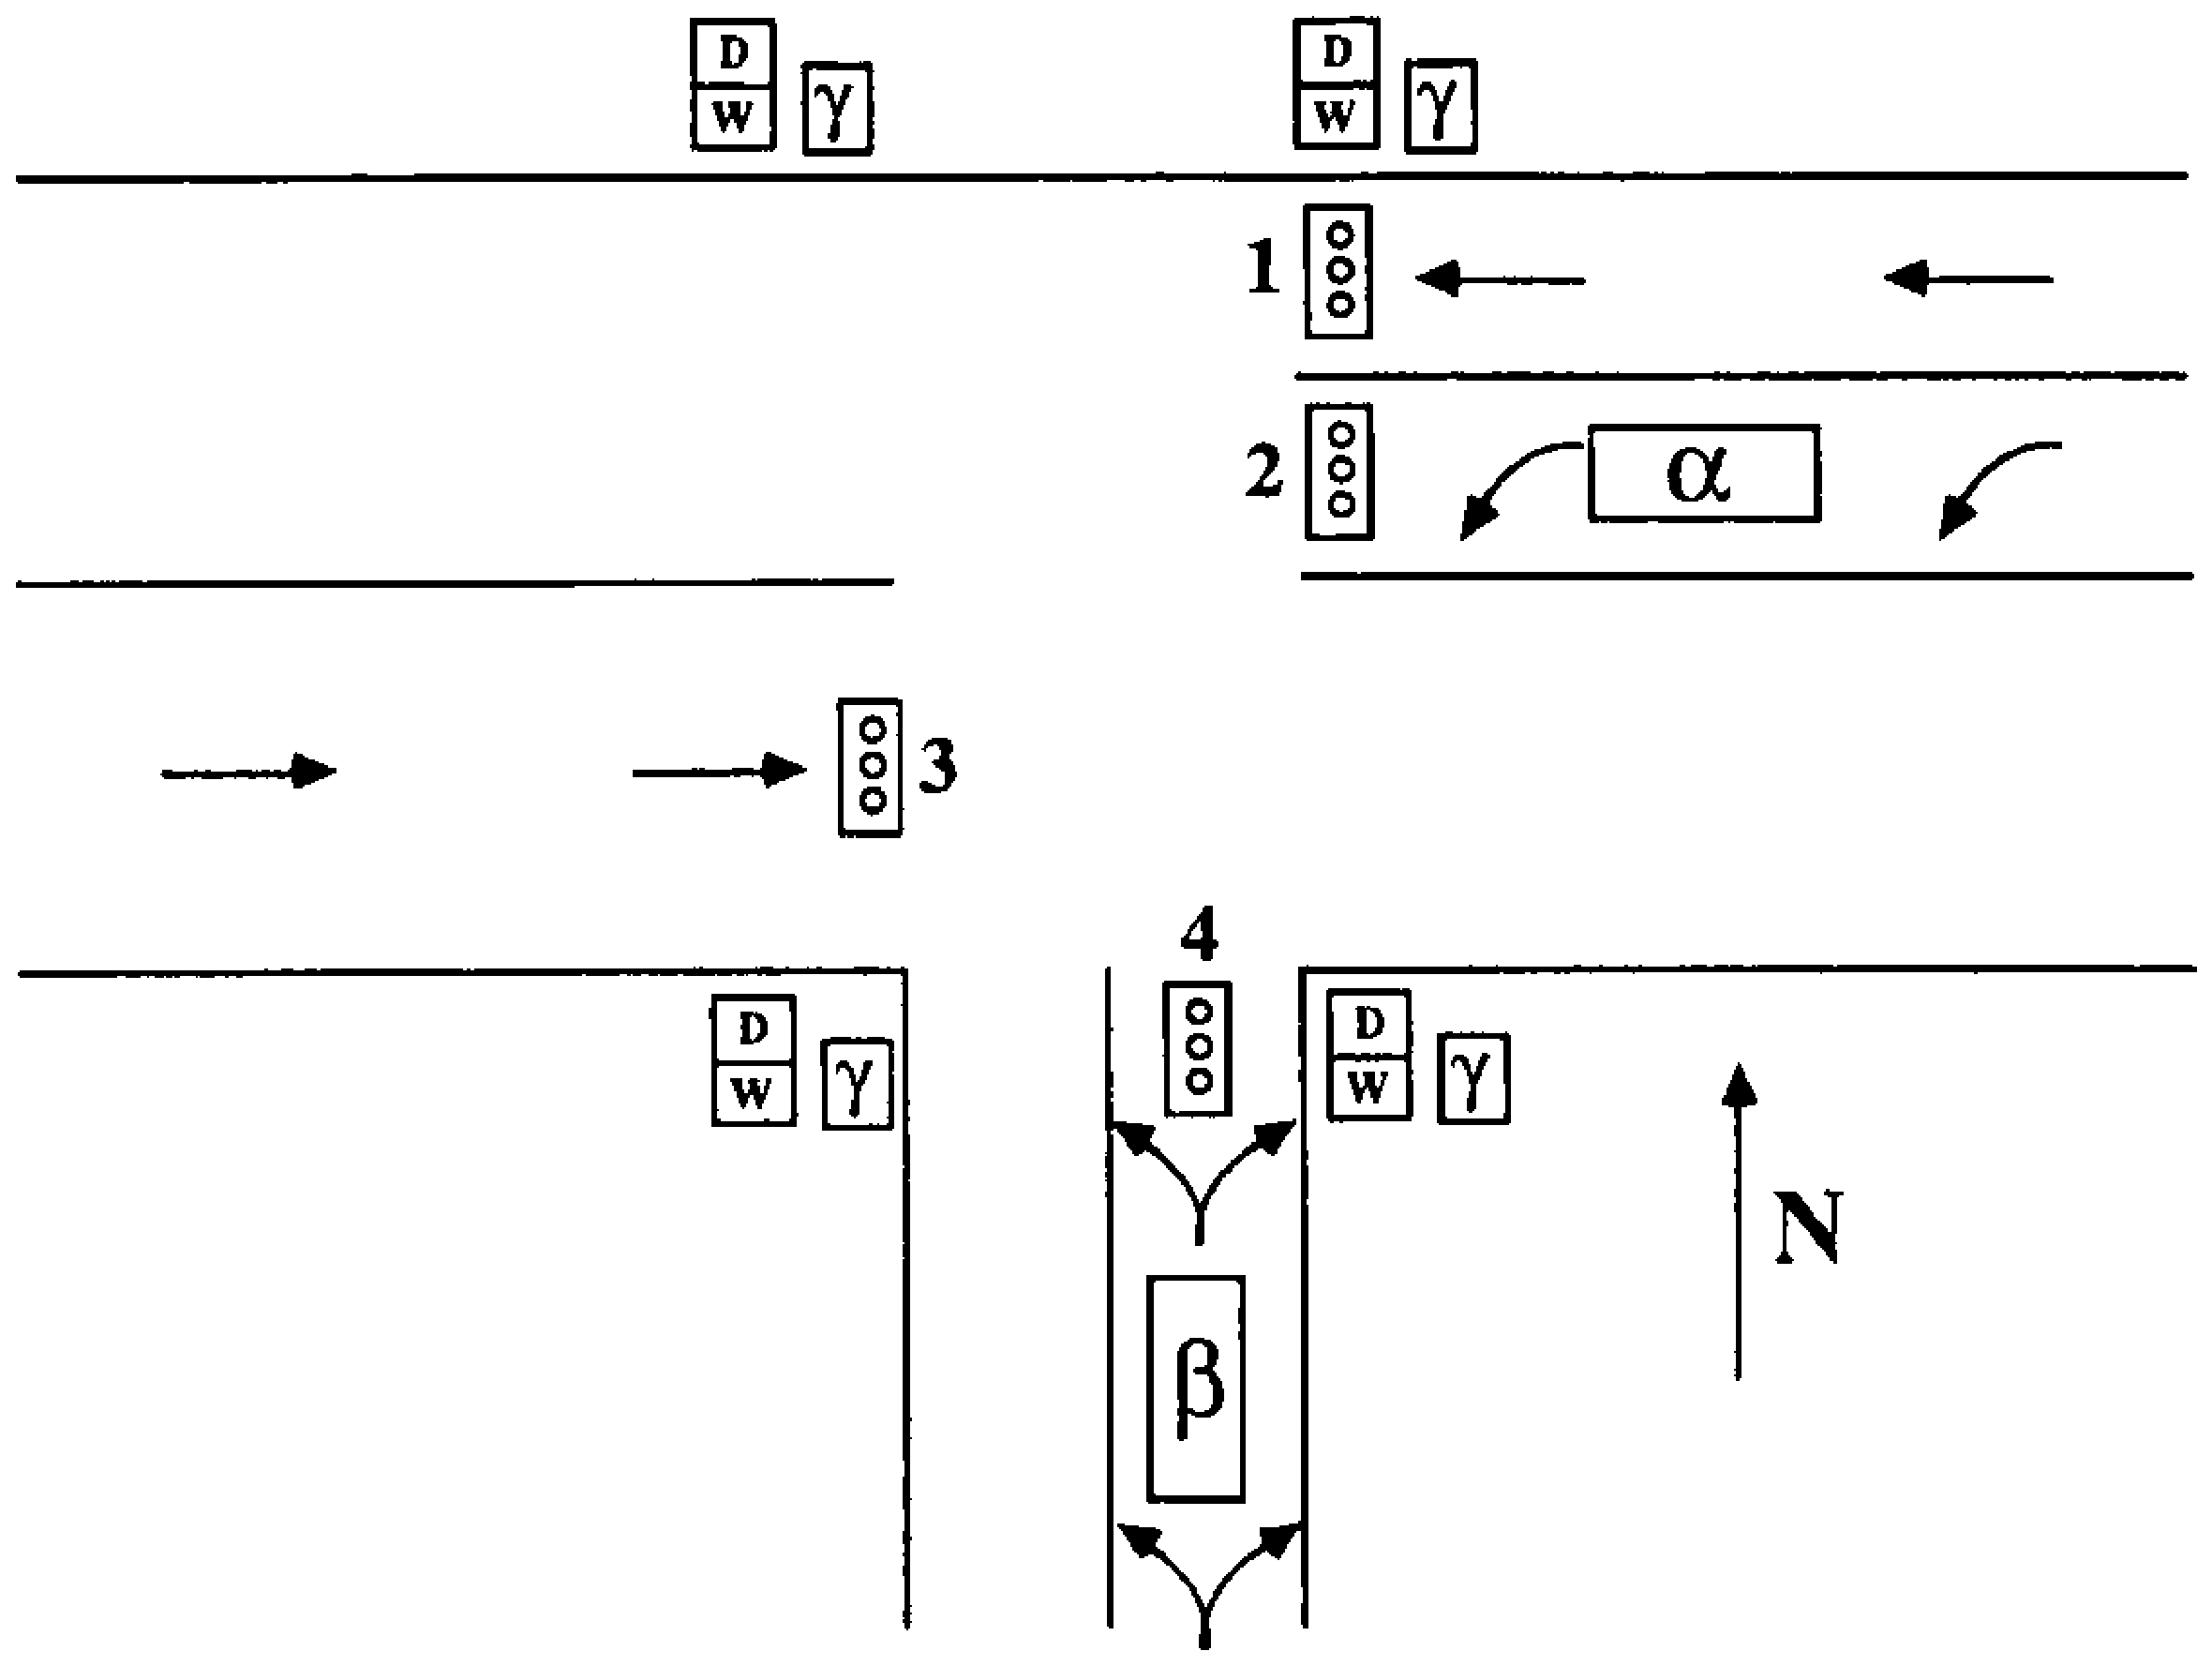
\epsfig{figure=ToFAfigures/fig7-19.eps,width=4.5in}}
\caption{The intersection discussed in Exercise 7.39}\label{fig-7.19}
\end{figure}
\begin{enumerate}
\item Define the new input and output alphabets.
\item Draw a Moore machine that implements this scenario.
\item Draw a Mealy machine that implements this scenario.
\end{enumerate}

\item Consider an intersection similar to that described in Example 7.16, as
shown in Figure \ref{fig-7.20}. There are now four left-turn signals in addition to the
four straight-ahead signals and additional input sensors $\gamma$ and $\delta$
for the other left-turn lanes. Assume that a normal alternation of
straight-ahead traffic is carried out, with no left turns indicated unless the
corresponding sensor is activated. Further assume that left-turn traffic will be
allowed to precede the opposing traffic.
\begin{enumerate}
\item Define the new input and output alphabets.
\item Draw a Moore machine that implements this scenario.
\item Draw a Mealy machine that implements this scenario.
\end{enumerate}
% Figure 7.20
\begin{figure}
\centerline{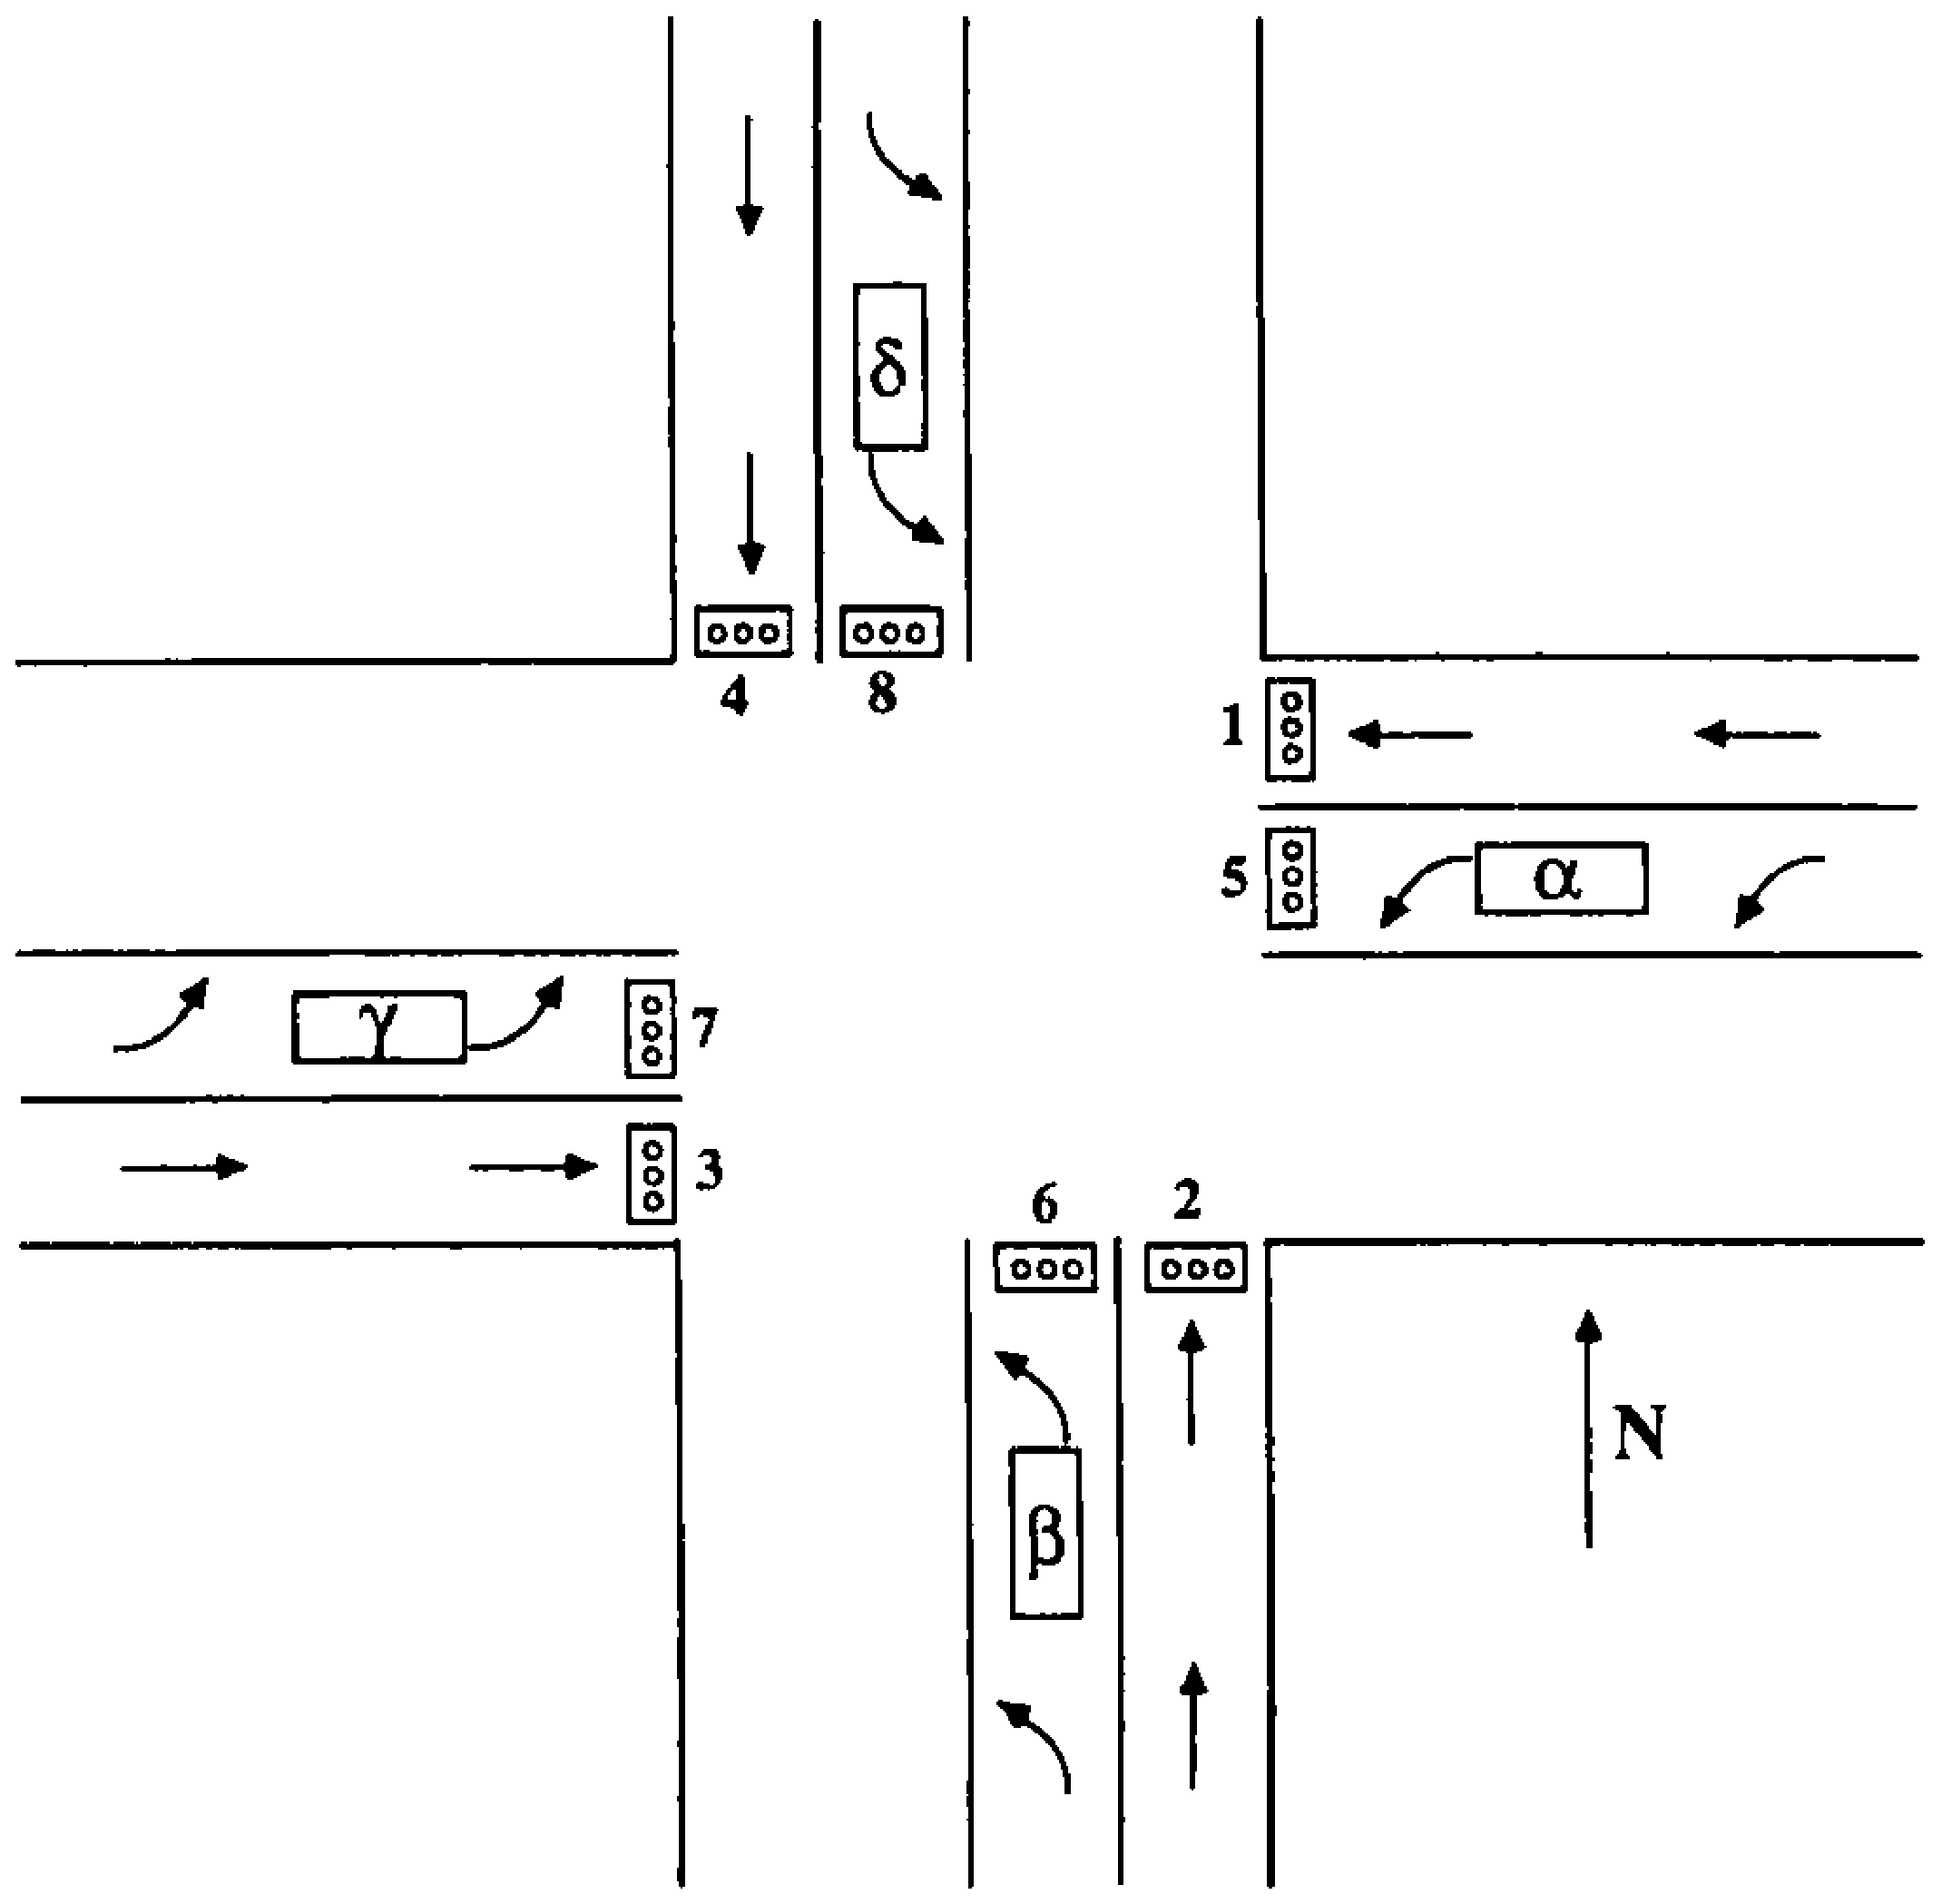
\epsfig{figure=ToFAfigures/fig7-20.eps,width=4.5in}}
\caption{The intersection discussed in Exercise 7.40}\label{fig-7.20}
\end{figure}

\item Consider an adder similar to the one in Example 7.15, but which instead
models addition in base 3.
\begin{enumerate}
\item Define the input and output alphabets.
\item Draw a Mealy machine that performs this addition.
\item Draw a Moore machine that performs this addition.
\item Draw a circuit that will implement the transducer built in part (b); use
both \<EOS\> and \<SOS\>.
\end{enumerate}

\item Consider an adder similar to the one in Example 7.15, but which models
addition in base 10.
\begin{enumerate}
\item Define the input and output alphabets.
\item Define the sextuple of a Mealy machine that performs this addition (by
indicating the output and transitions by concise formulas, rather than writing
out the 200 entries in the tables).
\item Define the sextuple of a Moore machine that performs this addition.
\item Draw a circuit that will implement the transducer built in part (b); use
both \<EOS\> and \<SOS\>.
\end{enumerate}

\item Consider a function $f_4$ implementing addition in a manner similar to
the function described by the transducer in Example 7.15, but that scans the
characters (that is, columns of digits) from left to right (rather than right to
left as in Example 7.15). Argue that $f_4$ is not FTD.

\item Given a MSM $M$, prove the following statements from Theorem \ref{thm-7.9}:
\begin{enumerate}
\item $M/\!\!_{E_M}$ is equivalent to $M$.
\item $M/\!\!_{E_M}$ is reduced.
\item If $M$ is connected, so is $M/\!\!_{E_M}$.
\end{enumerate}

\item Given a FTD function $f$, prove that the minimal Moore machine
corresponding to $f$ must be reduced.

\item Given a MSM $M$, prove the following statements from Theorem \ref{thm-7.10}:
\begin{enumerate}
\item A necessary and sufficient condition for $M$ to be minimal is that $M$ is
both reduced and connected.
\item $M^c/\!\!_{E_{M^c}}$ is minimal.
\end{enumerate}

\item Given MSMs $A=\langle\Sigma,\Gamma,S_A,s_{0_A},\delta_A,\omega_A\rangle$
and $B=\langle\Sigma,\Gamma,S_B,s_{0_B},\delta_B,\omega_B\rangle$, and a
homomorphism $\mu$$:\ S_A \rightarrow S_B$, prove the following statements from
Lemma \ref{lmm-7.5} and Corollary \ref{cor-7.9}:
\begin{enumerate}
\item $(\forall s \in S_A)(\forall x \in \Sigma^*)(\mu(\DBAR_A(s,x)) =
	\DBAR_B(\mu(s),x))$.
\item $(\forall s \in S_A)(\forall x \in \Sigma^*)(\OBAR_A(s,x) =
	\OBAR_B(\mu(s),x)))$.
\item $A$ is equivalent to $B$; that is, $f_A = f_B$.
\end{enumerate}

\item Prove Corollary \ref{cor-7.10}.

\item Prove Corollary \ref{cor-7.11}.

\item Given a FST $M=\langle\Sigma,\Gamma,S,s_0,\delta,\omega\rangle$ and
$M/\!\!_{E_M}=\langle\Sigma,\Gamma,S_{E_M},s_{0_{E_M}},\delta_{E_M},\omega_{E_M}
\rangle$ defined by
\begin{center}\begin{tabular}{ll}
$S_{E_M} =\{[s]_{E_M}$ $|$ $s \in S\}$ \\
$s_{0_{E_M}} = [s_0]_{E_M}$
\end{tabular}\end{center}
$\delta_{E_M}$ is defined by
\[ (\forall a \in \Sigma)(\forall [s]_{E_M} \in S_{E_M})(\delta_{E_M}([s]_{E_M},
	\pmb{a}) = [\delta(s,\pmb{a})]_{E_M}) \]
and $\omega_{E_M}$ is defined by
\[ (\forall\pmb{a}\in\Sigma)(\forall [s]_{E_M} \in S_{E_M})(\omega_{E_M}
	([s]_{E_M},\pmb{a}) = \omega(s,\pmb{a})) \]
\begin{enumerate}
\item Show that $\delta_{E_M}$ is well defined.
\item Show that $\omega_{E_M}$ is well defined.
\end{enumerate}

\item Given a MSM $M=\langle\Sigma,\Gamma,S,s_0,\delta,\omega\rangle$ and
$M/\!\!_{E_M}=\langle\Sigma,\Gamma,S_{E_M},s_{0_{E_M}},\delta_{E_M},\omega_{E_M}
\rangle$ defined by
\begin{center}\begin{tabular}{ll}
$S_{E_M} =\{[s]_{E_M}$ $|$ $s \in S\}$ \\
$s_{0_{E_M}} = [s_0]_{E_M}$
\end{tabular}\end{center}
$\delta_{E_M}$ is defined by
\[ (\forall a \in \Sigma)(\forall [s]_{E_M} \in S_{E_M})(\delta_{E_M}([s]_{E_M},
	\pmb{a}) = [\delta(s,\pmb{a})]_{E_M}) \]
and $\omega_{E_M}$ is defined by
\[ (\forall [s]_{E_M} \in S_{E_M})(\omega_{E_M}([s]_{E_M}) = \omega(s)) \]
\begin{enumerate}
\item Show that $\delta_{E_M}$ is well defined.
\item Show that $\omega_{E_M}$ is well defined.
\end{enumerate}

\item Consider the following assertion: If there is an isomorphism from $A$ to
$B$ and $A$ is connected, then $B$ must also be connected.
\begin{enumerate}
\item Prove that this is true for isomorphisms between Mealy machines.
\item Prove that this is true for isomorphisms between Moore machines.
\end{enumerate}

\item Consider the following assertion: If there is an isomorphism from $A$ to
$B$ and $B$ is connected, then $A$ must also be connected.
\begin{enumerate}
\item Prove that this is true for isomorphisms between Mealy machines.
\item Prove that this is true for isomorphisms between Moore machines.
\end{enumerate}

\item Consider the following assertion: If there is a homomorphism from $A$ to
$B$ and $A$ is connected, then $B$ must also be connected.
\begin{enumerate}
\item Give an example of two Mealy machines for which this assertion is false.
\item Give an example of two Moore machines for which this assertion is false.
\end{enumerate}

\item Consider the following assertion: If there is a homomorphism from $A$ to
$B$ and $B$ is connected, then $A$ must also be connected.
\begin{enumerate}
\item Give an example of two Mealy machines for which this assertion is false.
\item Give an example of two Moore machines for which this assertion is false.
\end{enumerate}

\item Assume $A$ and $B$ are connected FSTs and that there exists an isomorphism
$\psi$ from $A$ to $B$ and an isomorphism $\mu$ from B to A. Prove that $\psi =
\mu^{-1}$.

\item Assume $A$ and $B$ are FSTs and there exists an isomorphism $\psi$ from
$A$ to $B$ and an isomorphism $\mu$ from $B$ to $A$. Give an example for which
$\psi \not= \mu^{-1}$.

\item Give an example of a three-state MSM for which $E_{0A}$ has only one
equivalence class. Is it possible for $E_{0A}$ to be different from $E_{1A}$ in
such a machine? Explain.

\item \begin{enumerate}
\item Give an example of a Mealy machine for which $M$ is \emph{not} connected
and $M/\!\!_{E_M}$ is not connected.
\item Give an example of a Mealy machine for which $M$ is \emph{not} connected
but $M/\!\!_{E_M}$ is connected.
\end{enumerate}

\item \begin{enumerate}
\item Give an example of a Moore machine for which $M$ is \emph{not} connected
and $M/\!\!_{E_M}$ is not connected.
\item Give an example of a Moore machine for which $M$ is \emph{not} connected
but $M/\!\!_{E_M}$ is connected.
\end{enumerate}

\item For a homomorphism $\mu$$:\ S_A \rightarrow S_B$ between two Mealy machines
\[ A=\langle\Sigma,\Gamma,S_A,s_{0_A},\delta_A,\omega_A\rangle\qquad\text{and}
	\qquad B=\langle\Sigma,\Gamma,S_B,s_{0_B},\delta_B,\omega_B\rangle, \]
prove $(\forall s,t \in S_A)(\mu(s) E_B \mu(t) \Leftrightarrow s E_A t)$.

\item For a homomorphism $\mu$$:\ S_A \rightarrow S_B$ between two Moore machines
\[ A=\langle\Sigma,\Gamma,S_A,s_{0_A},\delta_A,\omega_A\rangle\qquad\text{and}
	\qquad B=\langle\Sigma,\Gamma,S_B,s_{0_B},\delta_B,\omega_B\rangle, \]
prove $(\forall s,t \in S_A)(\mu(s) E_B \mu(t) \Leftrightarrow s E_A t)$.

\item \begin{enumerate}
\item Give an example of a FST for which $A$ is \emph{not} reduced and $A^c$ is
not reduced.
\item Give an example of a FST for which $A$ is \emph{not} reduced and $A^c$
\emph{is} reduced.
\end{enumerate}

\item \begin{enumerate}
\item Give an example of a MSM for which $A$ is \emph{not} reduced and $A^c$ is
not reduced.
\item Give an example of a MSM for which $A$ is \emph{not} reduced and $A^c$
\emph{is} reduced.
\end{enumerate}

\item Isomorphism ($\cong$) is a relation in the set of all Mealy machines.
\begin{enumerate}
\item Prove that $\cong$ is a symmetric relation; that is, formally justify that
if there is an isomorphism from $A$ to $B$ then there is an isomorphism from $B$
to $A$.
\item Prove that $\cong$ is a reflexive relation.
\item Show that if $f$ and $g$ are isomorphisms, then $f \circ g$ is also an
isomorphism (whenever $f \circ g$ is defined).
\item From the results of parts (a), (b), and (c) given above, prove that
$\cong$ is an equivalence relation over the set of all Mealy machines.
\item Show that homomorphism is {\em not} an equivalence relation over the set of all
Mealy machines.
\end{enumerate}

\item \begin{enumerate}
\item Prove that $\cong$ is an equivalence relation in the set of all Moore
machines.
\item Show that homomorphism is {\em not} an equivalence relation over the set of all
Moore machines.
\end{enumerate}

\item Given a Mealy machine $M=\langle\Sigma,\Gamma,S,s_0,\delta,\omega\rangle$,
prove that there exists a homomorphism $\mu$ from $M$ to $M/\!\!_{E_M}$.

\item Given a Moore machine $M=\langle\Sigma,\Gamma,S,s_0,\delta,\omega\rangle$,
prove that there exists a homomorphism $\mu$ from $M$ to $M/\!\!_{E_M}$.

\item Consider the intersection presented in Example 7.16 and note that the
construction presented in Figure \ref{fig-7.15} prevents the transducer from leaving $s_2$
or $s_6$ while the appropriate sensor is active. The length of time spent in
each output configuration can be limited by replacing $s_2$ with a sequence of
states that ensures that the output configuration will change within, say, three
clock cycles (this is similar to the spirit in which $s_8$ was added). A similar
expansion can be made with regard to $s_6$. While this would not be a likely
problem if the side street were not heavily traveled, higher traffic situations
would require a different solution than that shown in Figure \ref{fig-7.15}.
\begin{enumerate}
\item Modify Figure \ref{fig-7.15} so that the output configuration can, when necessary,
remain at $\langle R,R,R,G\rangle$ for three clock cycles, but not for four
clock cycles.
\item Starting with the larger transducer found in part (a), make a similar
expansion to $s_6$.
\item Starting with the larger transducer found in part (a), make an expansion
to $s_6$ in such a way that the left-turn signal is guaranteed to be green for a
minimum of two clock cycles and a maximum of four clock cycles.
\end{enumerate}

\item Consider the intersection presented in Example 7.16 and note that the
construction presented in Figure \ref{fig-7.15} prevents the transducer from returning to
$s_0$ while either of the sensors is active. Thus, even if the length of time
spent in each output configuration was limited (see Exercise 7.69), left-turn
and northbound traffic could perpetually alternate without ever allowing the
east-west traffic to resume. This would not be a likely problem if the side
street were not heavily traveled, but higher traffic situations would require a
different solution than the one presented in Example 7.16.
\begin{enumerate}
\item Without adding any states to Figure \ref{fig-7.15}, modify the state transition
diagram so that east-west traffic will receive a green light occasionally.
\item By adding new states to Figure \ref{fig-7.15} (to remember the last lanes that had
the right of way), implement a controller that will ensure that no lane will get
a second green light if any other lane that has an active sensor has yet to
receive a green light. (It may be helpful to think of the east-west traffic as
having an implicit sensor that is always actively demanding service).
\end{enumerate}

\item Prove that if two Moore machines are homomorphic then they are equivalent.

\item Show that, for any FTD function $f$$:\ \Sigma^* \rightarrow \Sigma^*$,
\DSIG\ is closed under $f$.
\end{enumerate}
